\documentclass{patmorin}
\listfiles
\usepackage[utf8]{inputenc}
\usepackage{amsthm,amsmath,graphicx}
\usepackage{pat}
\usepackage[letterpaper]{hyperref}
\usepackage[table,dvipsnames]{xcolor}
%\usepackage[dvipsnames]{color}
\definecolor{linkblue}{named}{Blue}
\hypersetup{colorlinks=true, linkcolor=linkblue,  anchorcolor=linkblue,
citecolor=linkblue, filecolor=linkblue, menucolor=linkblue,
urlcolor=linkblue, pdfcreator=Me, pdfproducer=Me} \setlength{\parskip}{1ex}


\DeclareMathOperator{\sign}{sign}
\DeclareMathOperator{\xmax}{xmax}
\DeclareMathOperator{\xmin}{xmin}
\DeclareMathOperator{\ymax}{ymax}
\DeclareMathOperator{\ymin}{ymin}
\DeclareMathOperator{\survivors}{survivors}

\usepackage{array}


% To reduce space in lists
\usepackage{enumitem}  
\setlist{noitemsep}

%\usepackage[skip=0pt]{caption}

\title{\MakeUppercase{More Turán-Type Theorems for Triangles in Convex Point Sets}\thanks{This research is partially funded by NSERC.}}
\author{Authors TBD}


\newcommand{\taco}{\raisebox{-.1ex}{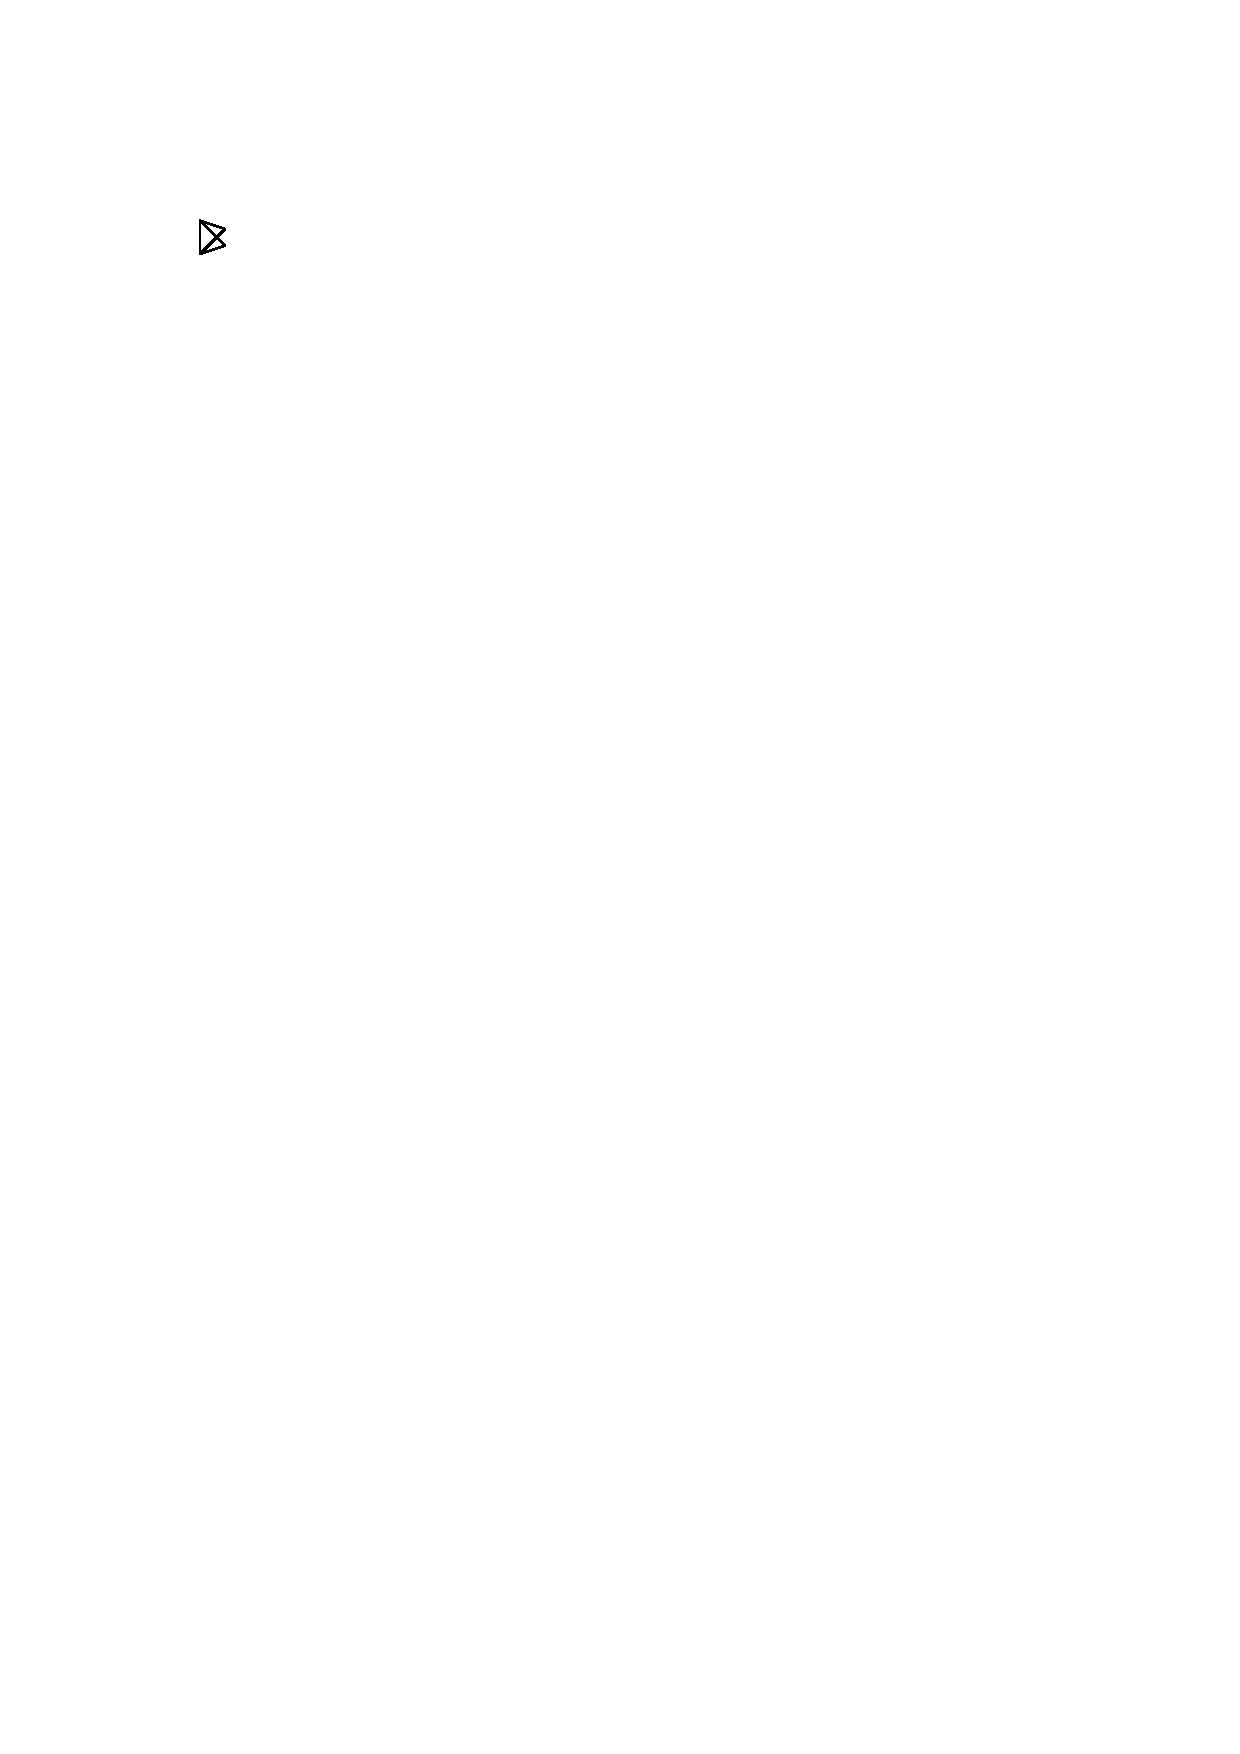
\includegraphics[height=1.6ex]{figs/triangles-edge-1}}}
\newcommand{\mariposa}{\raisebox{-.1ex}{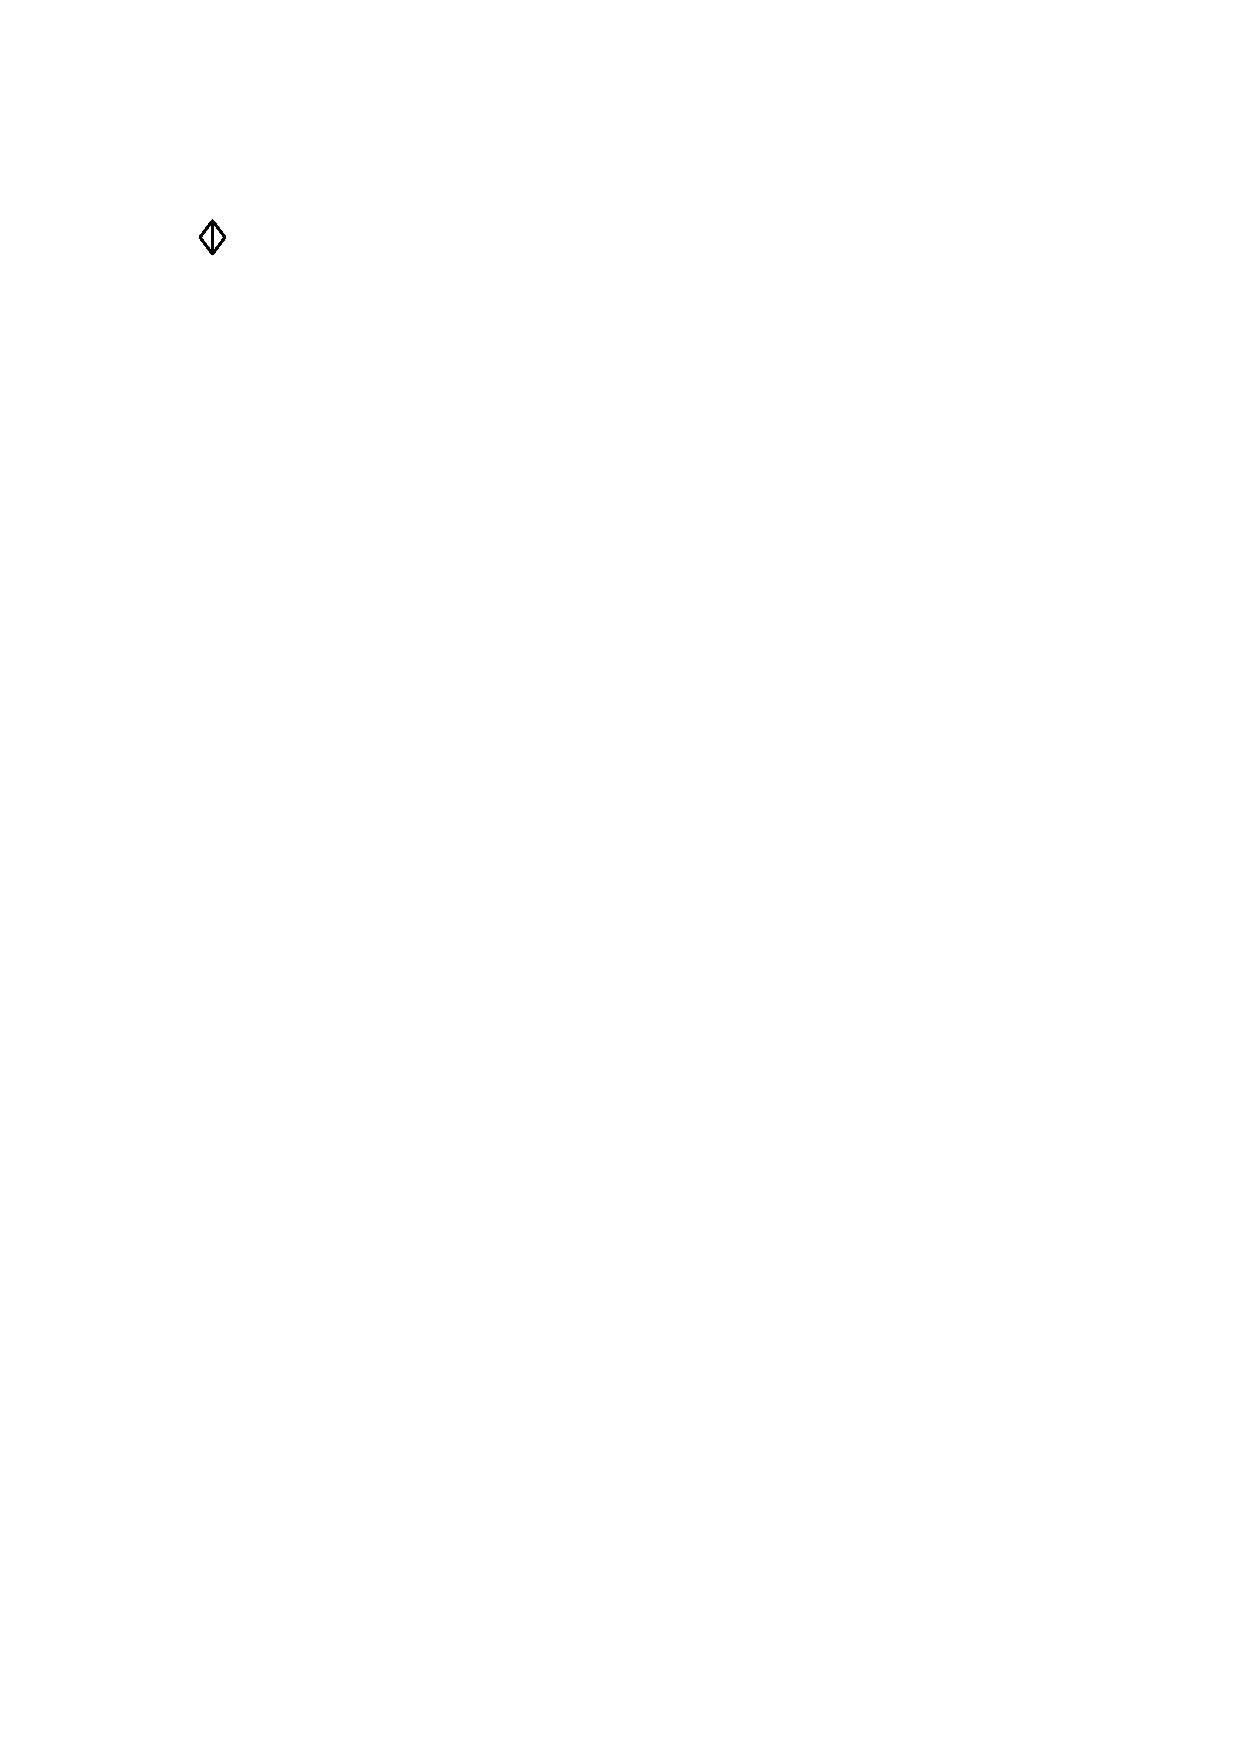
\includegraphics[height=1.6ex]{figs/triangles-edge-2}}}


\newcommand{\bat}{\raisebox{-.1ex}{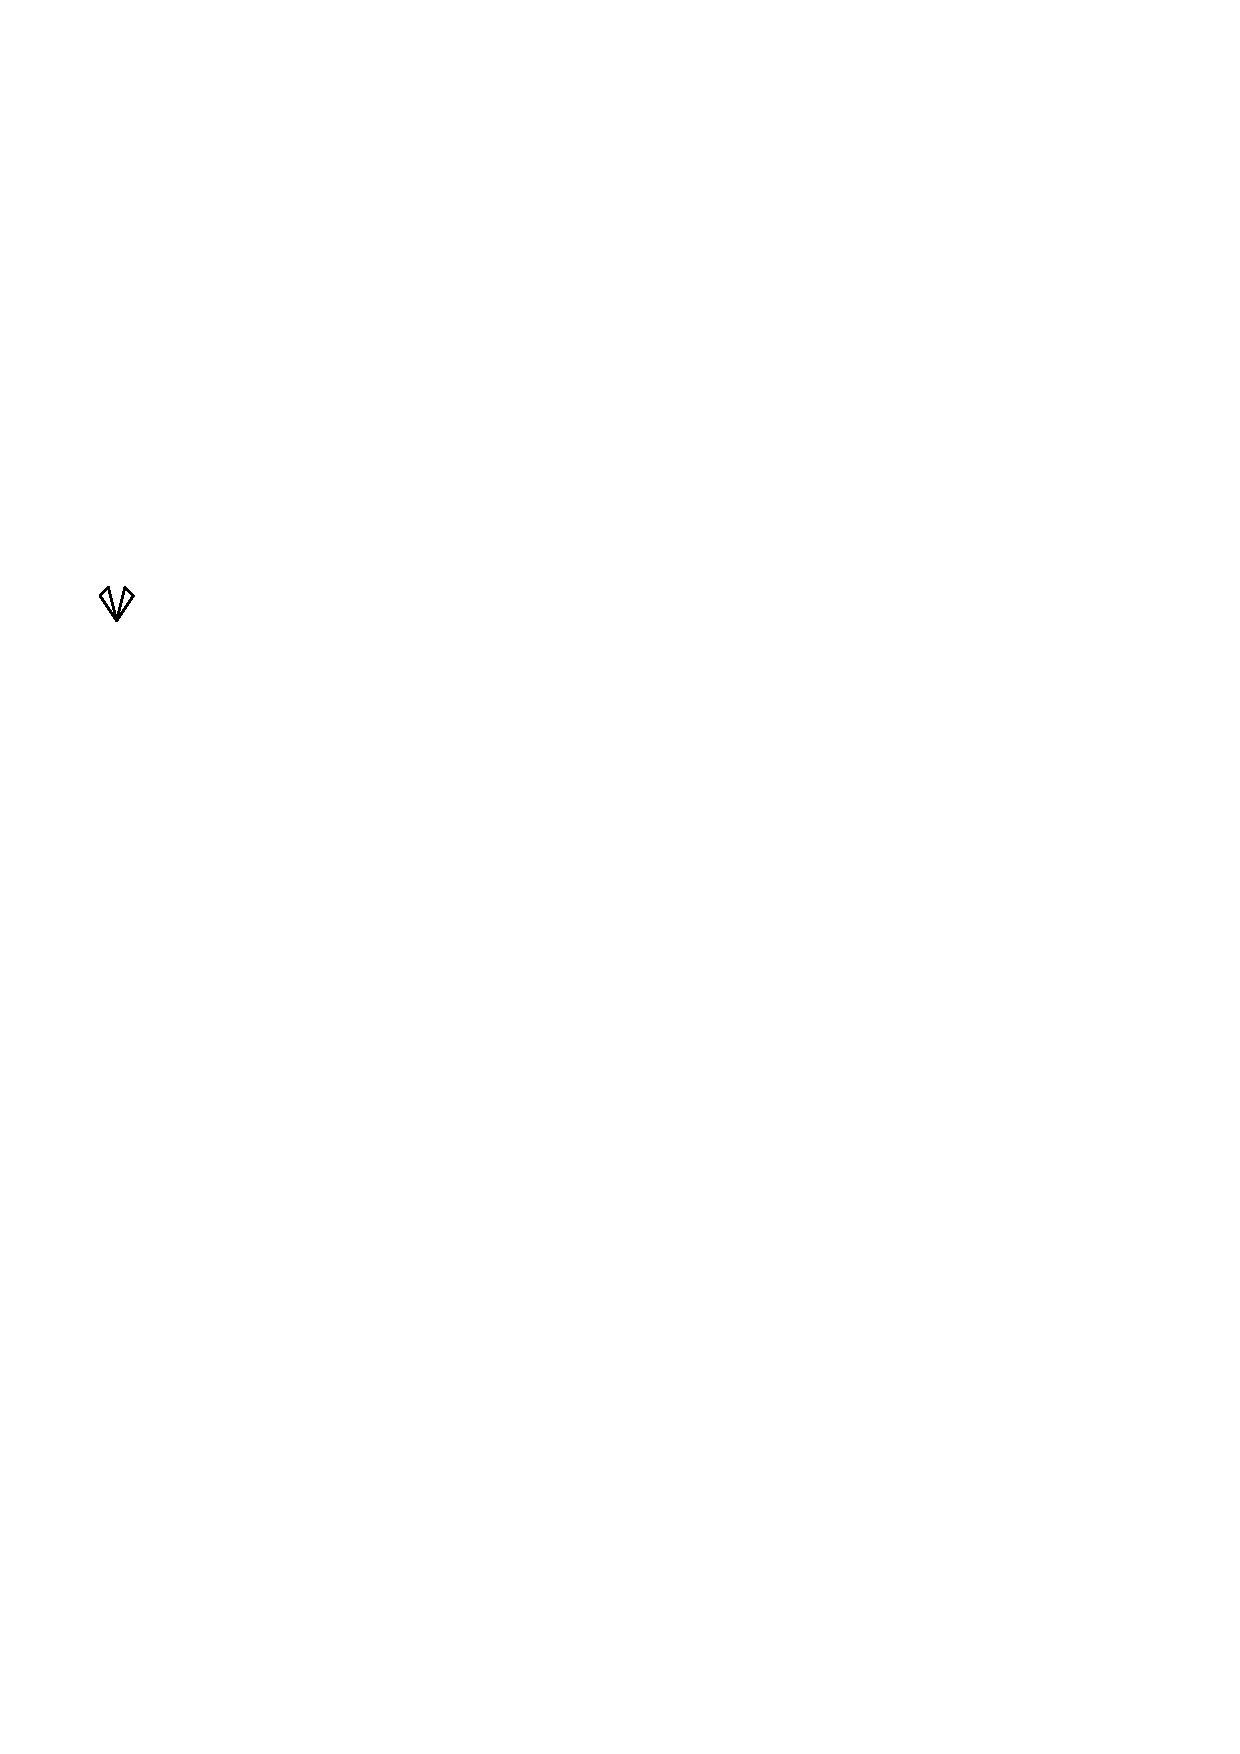
\includegraphics[height=1.6ex]{figs/triangles-vertex-1}}}
\newcommand{\nested}{\raisebox{-.1ex}{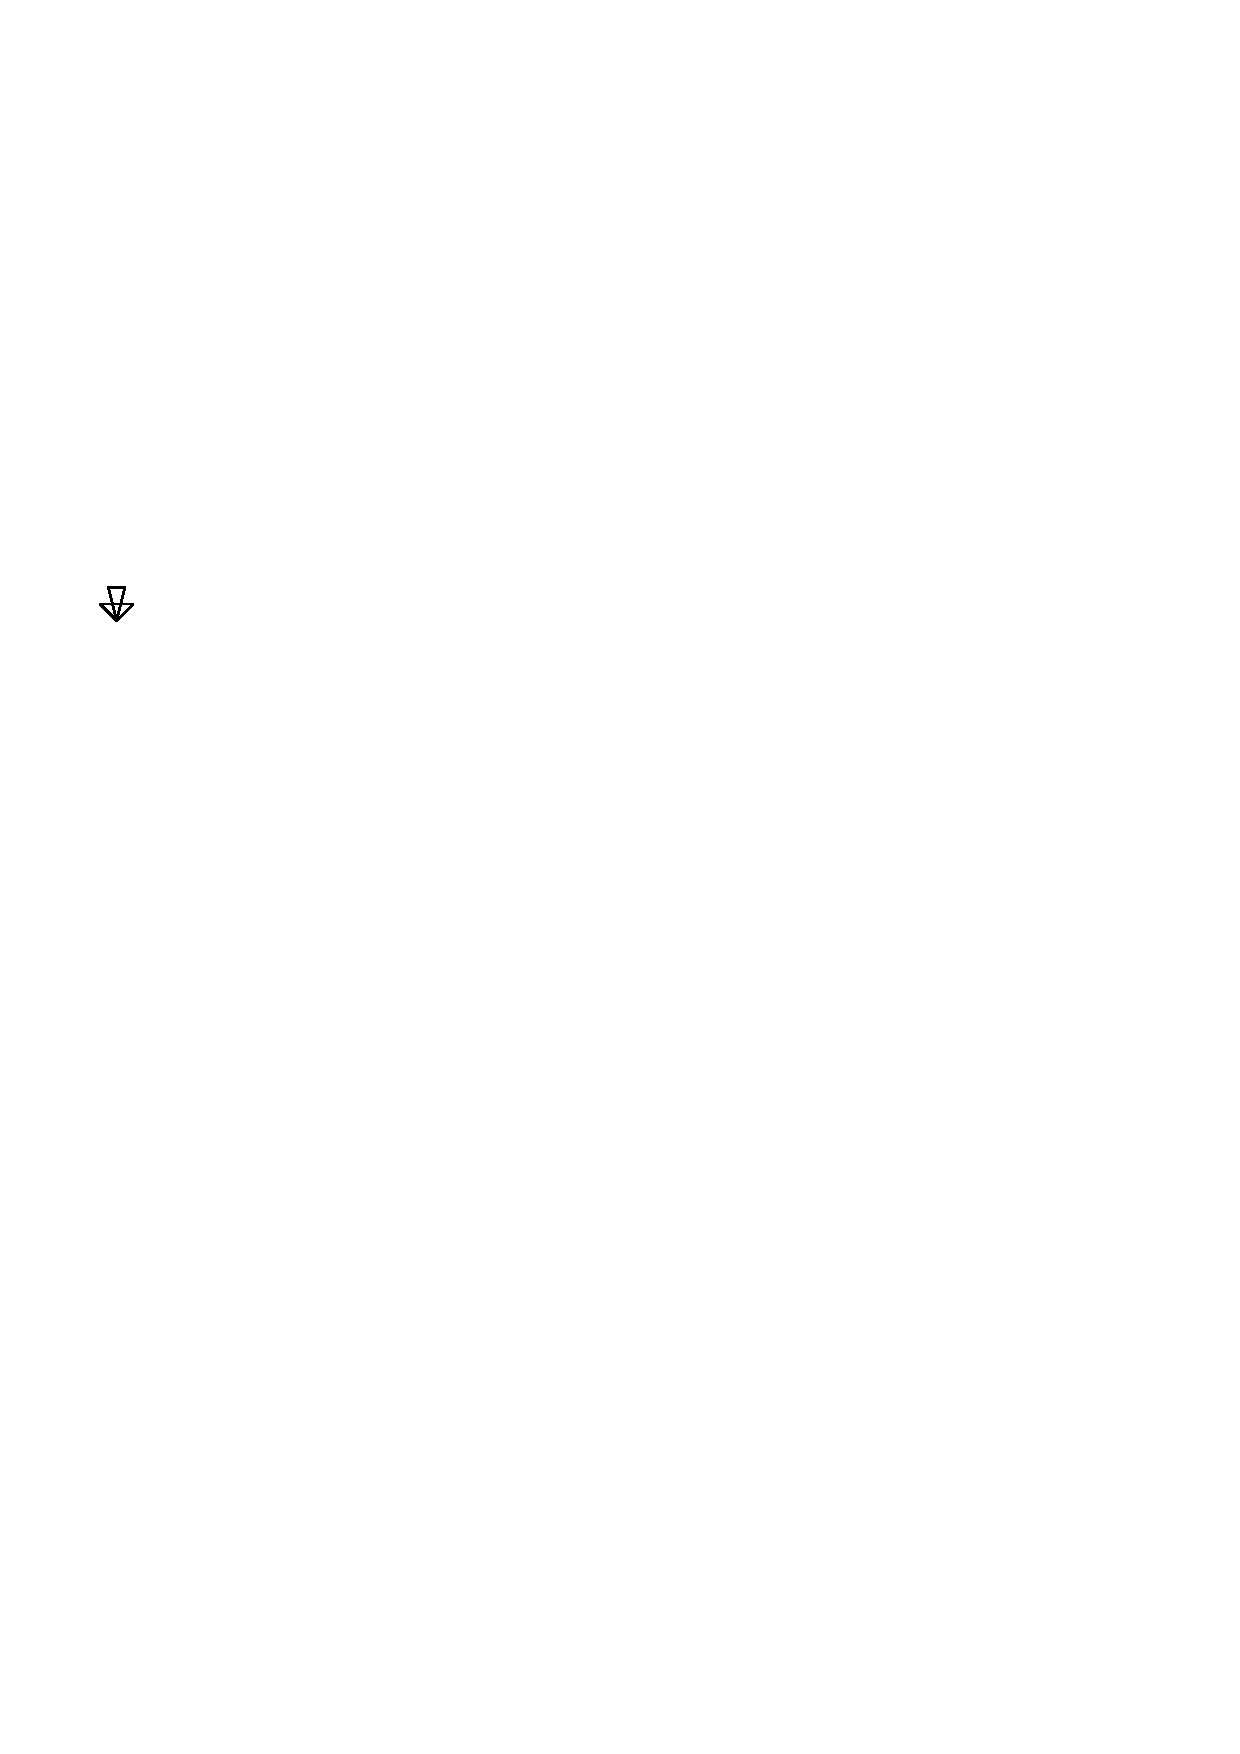
\includegraphics[height=1.6ex]{figs/triangles-vertex-2}}}
\newcommand{\crossing}{\raisebox{-.1ex}{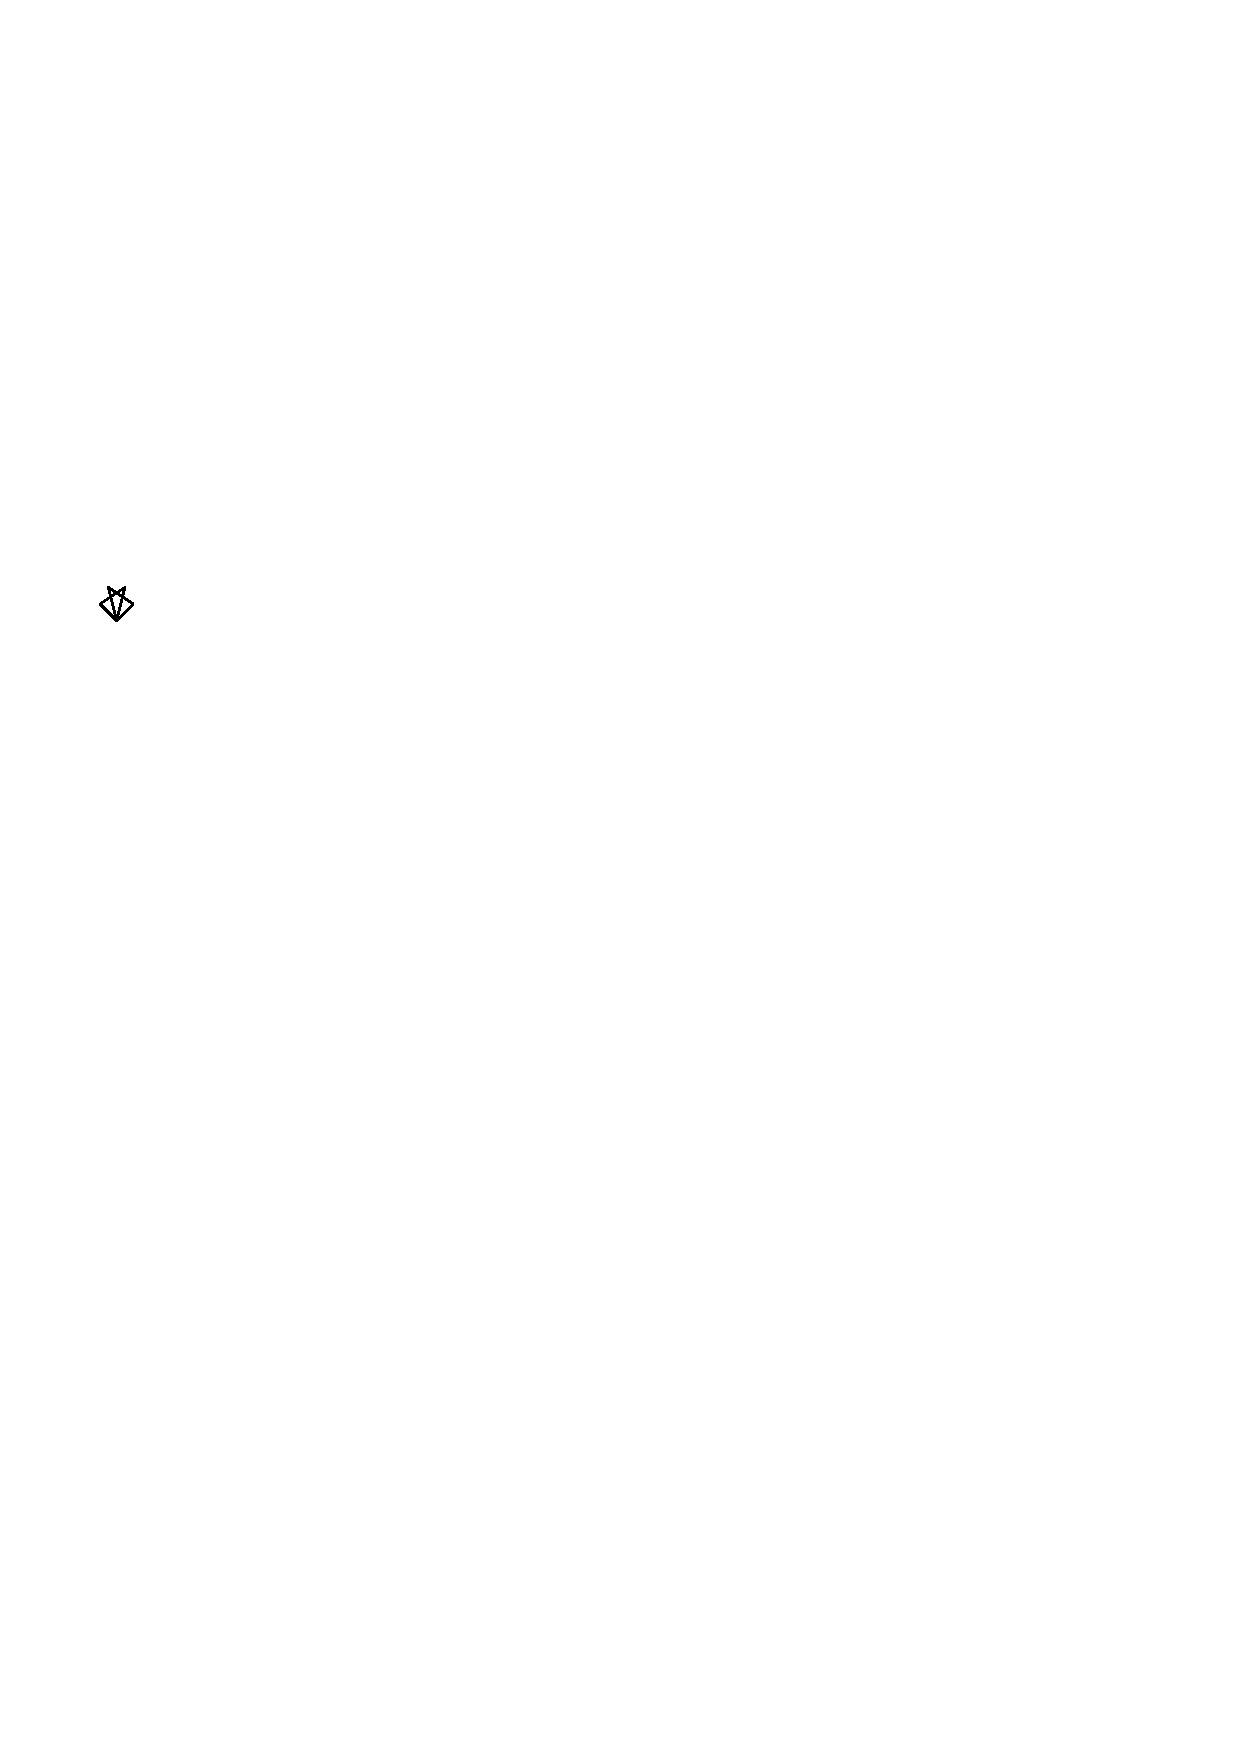
\includegraphics[height=1.6ex]{figs/triangles-vertex-3}}}

\newcommand{\ears}{\raisebox{-.1ex}{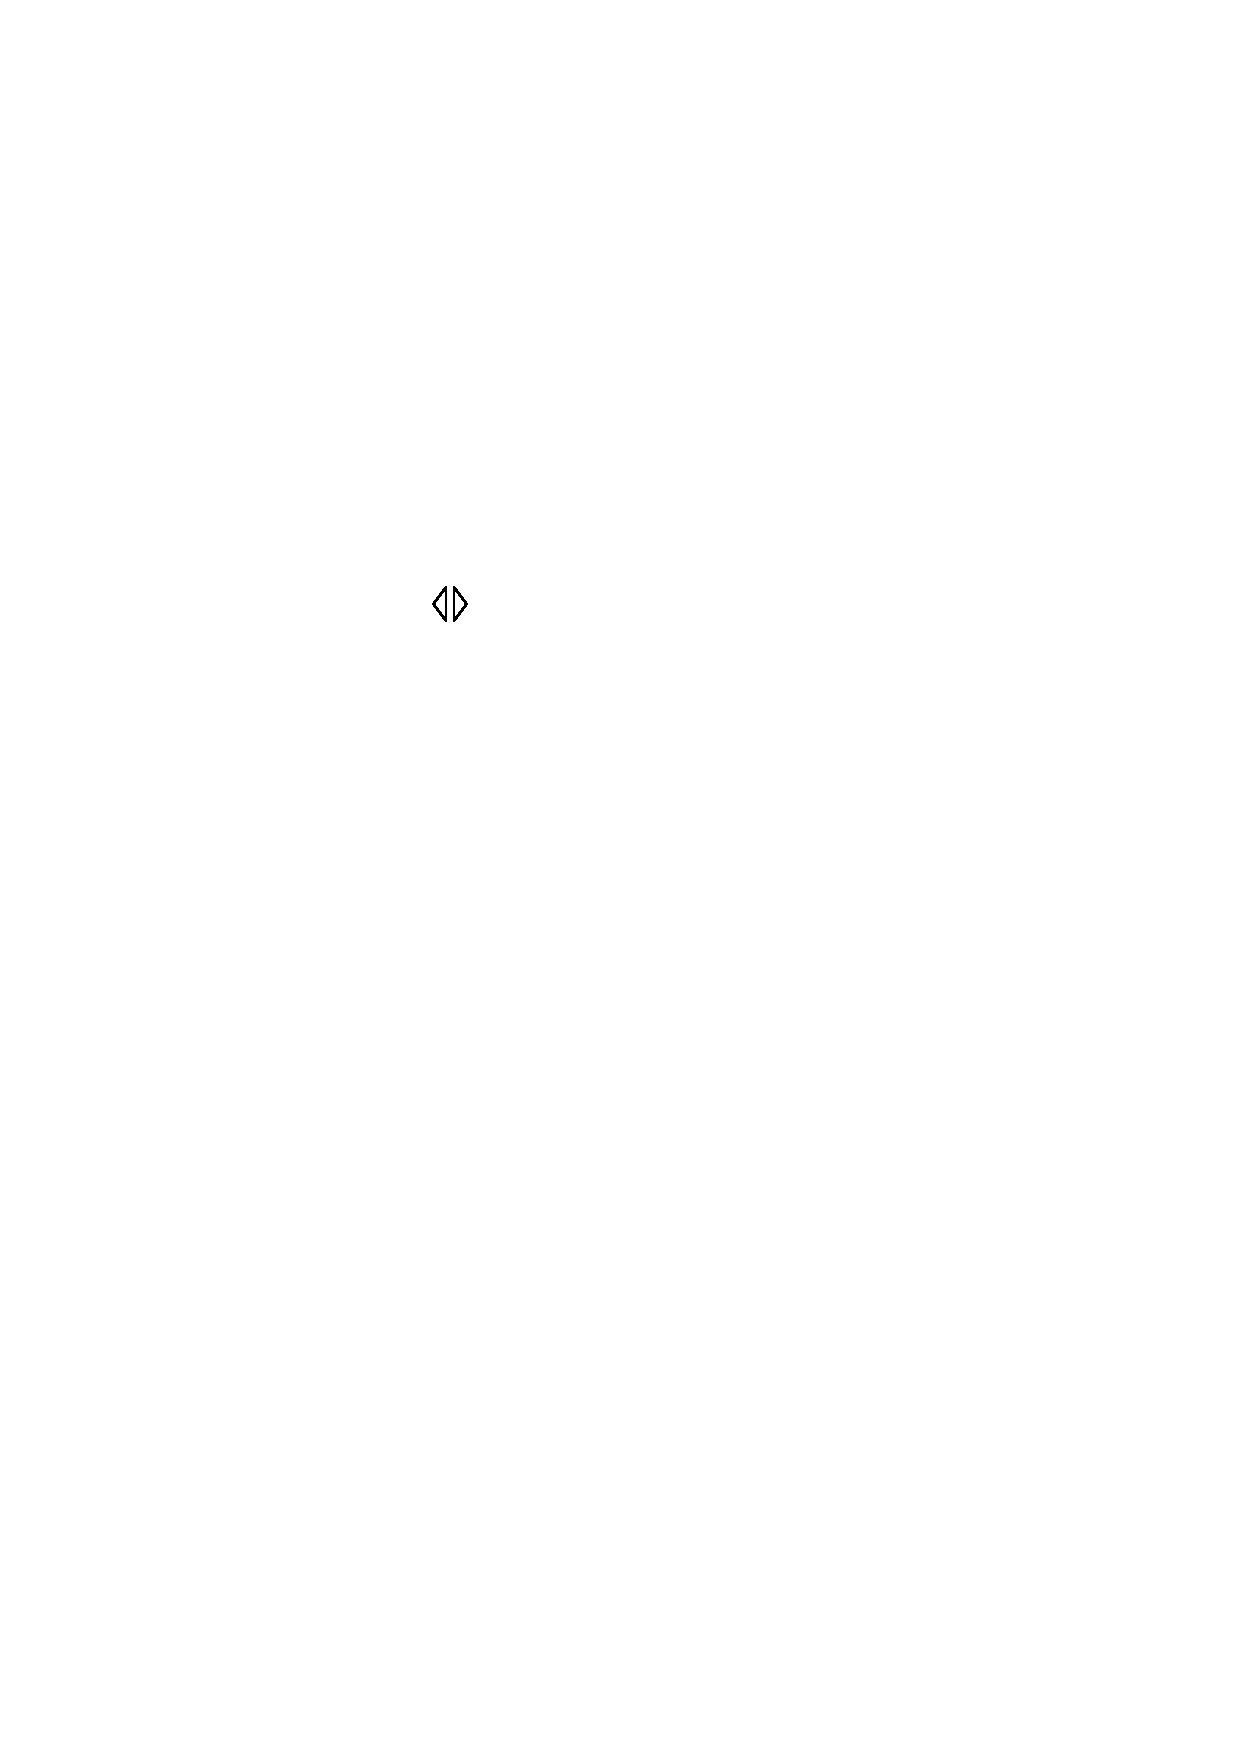
\includegraphics[height=1.6ex]{figs/triangles-disjoint-1}}}
\newcommand{\swords}{\raisebox{-.1ex}{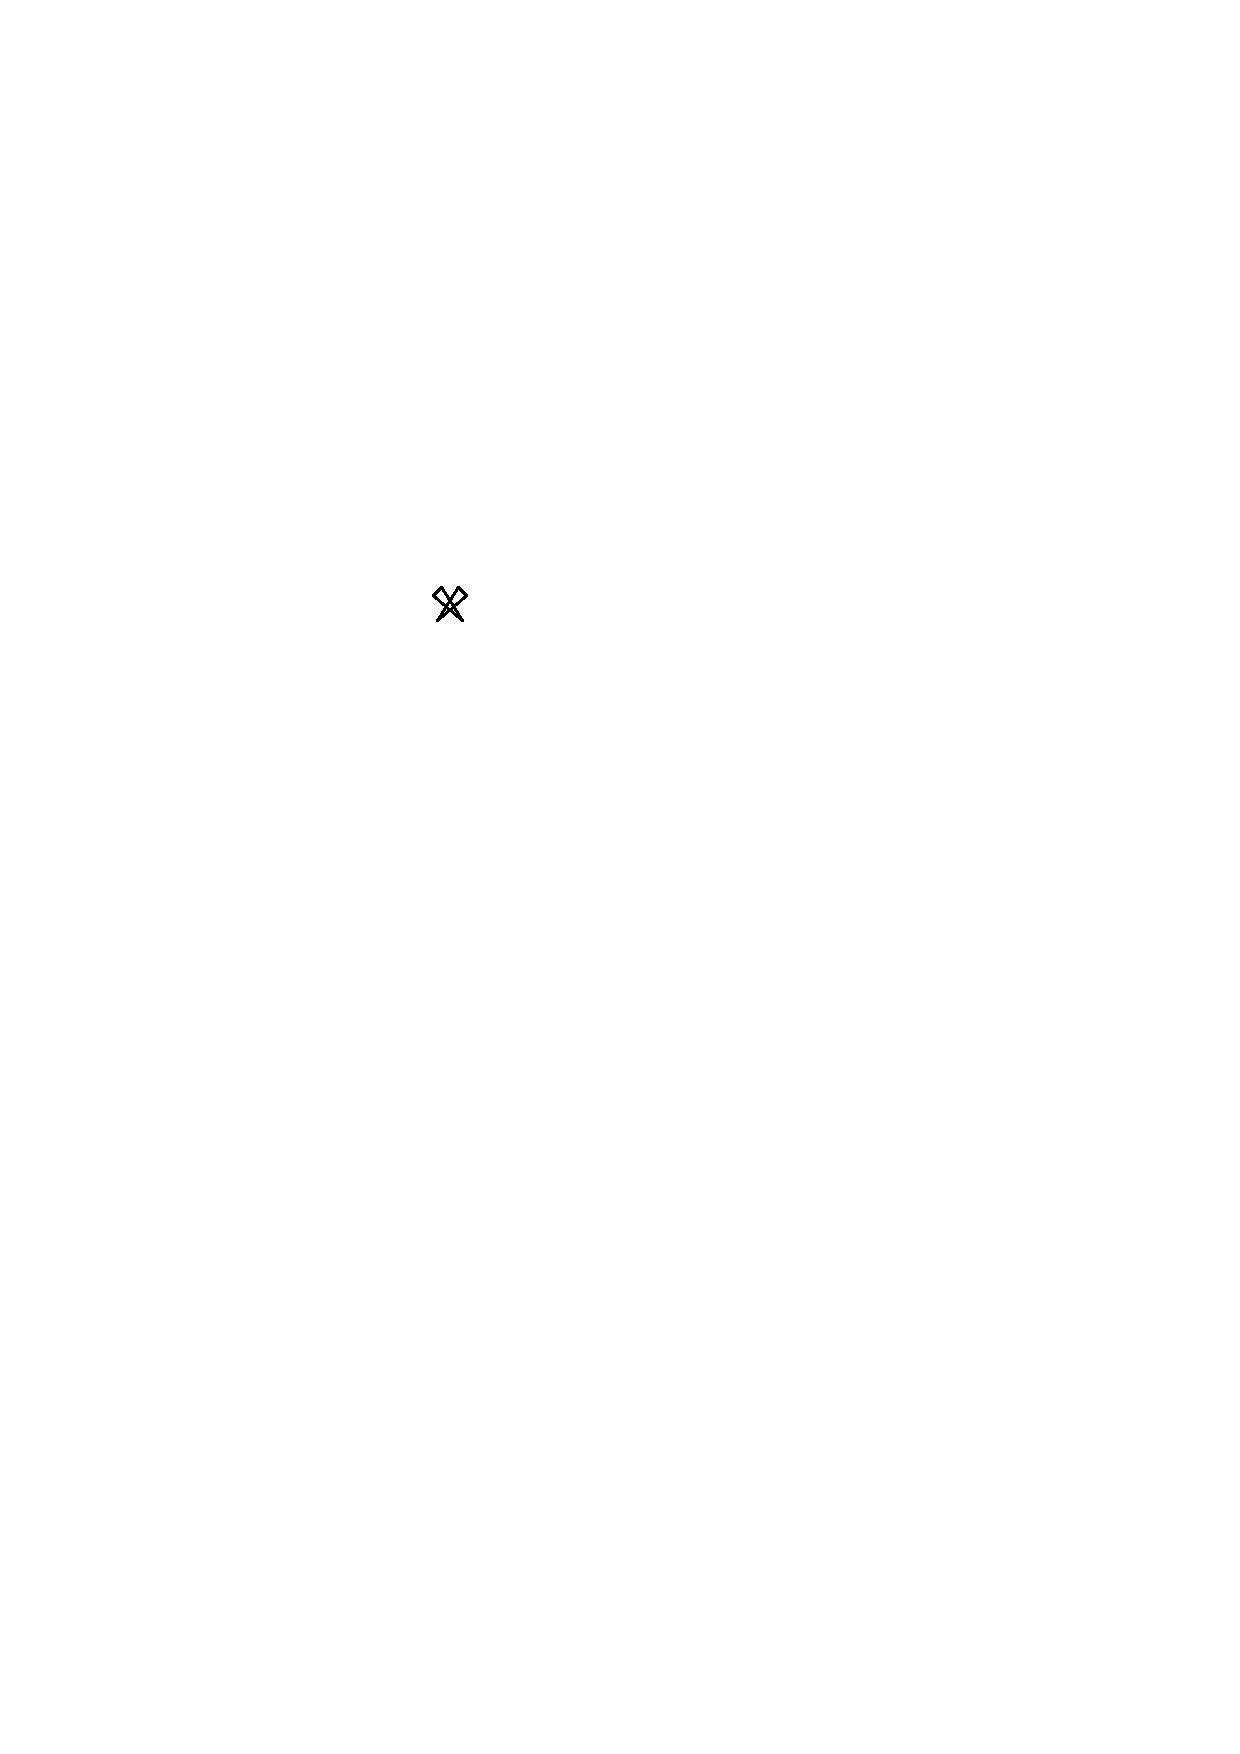
\includegraphics[height=1.6ex]{figs/triangles-disjoint-2}}}
\newcommand{\david}{\raisebox{-.1ex}{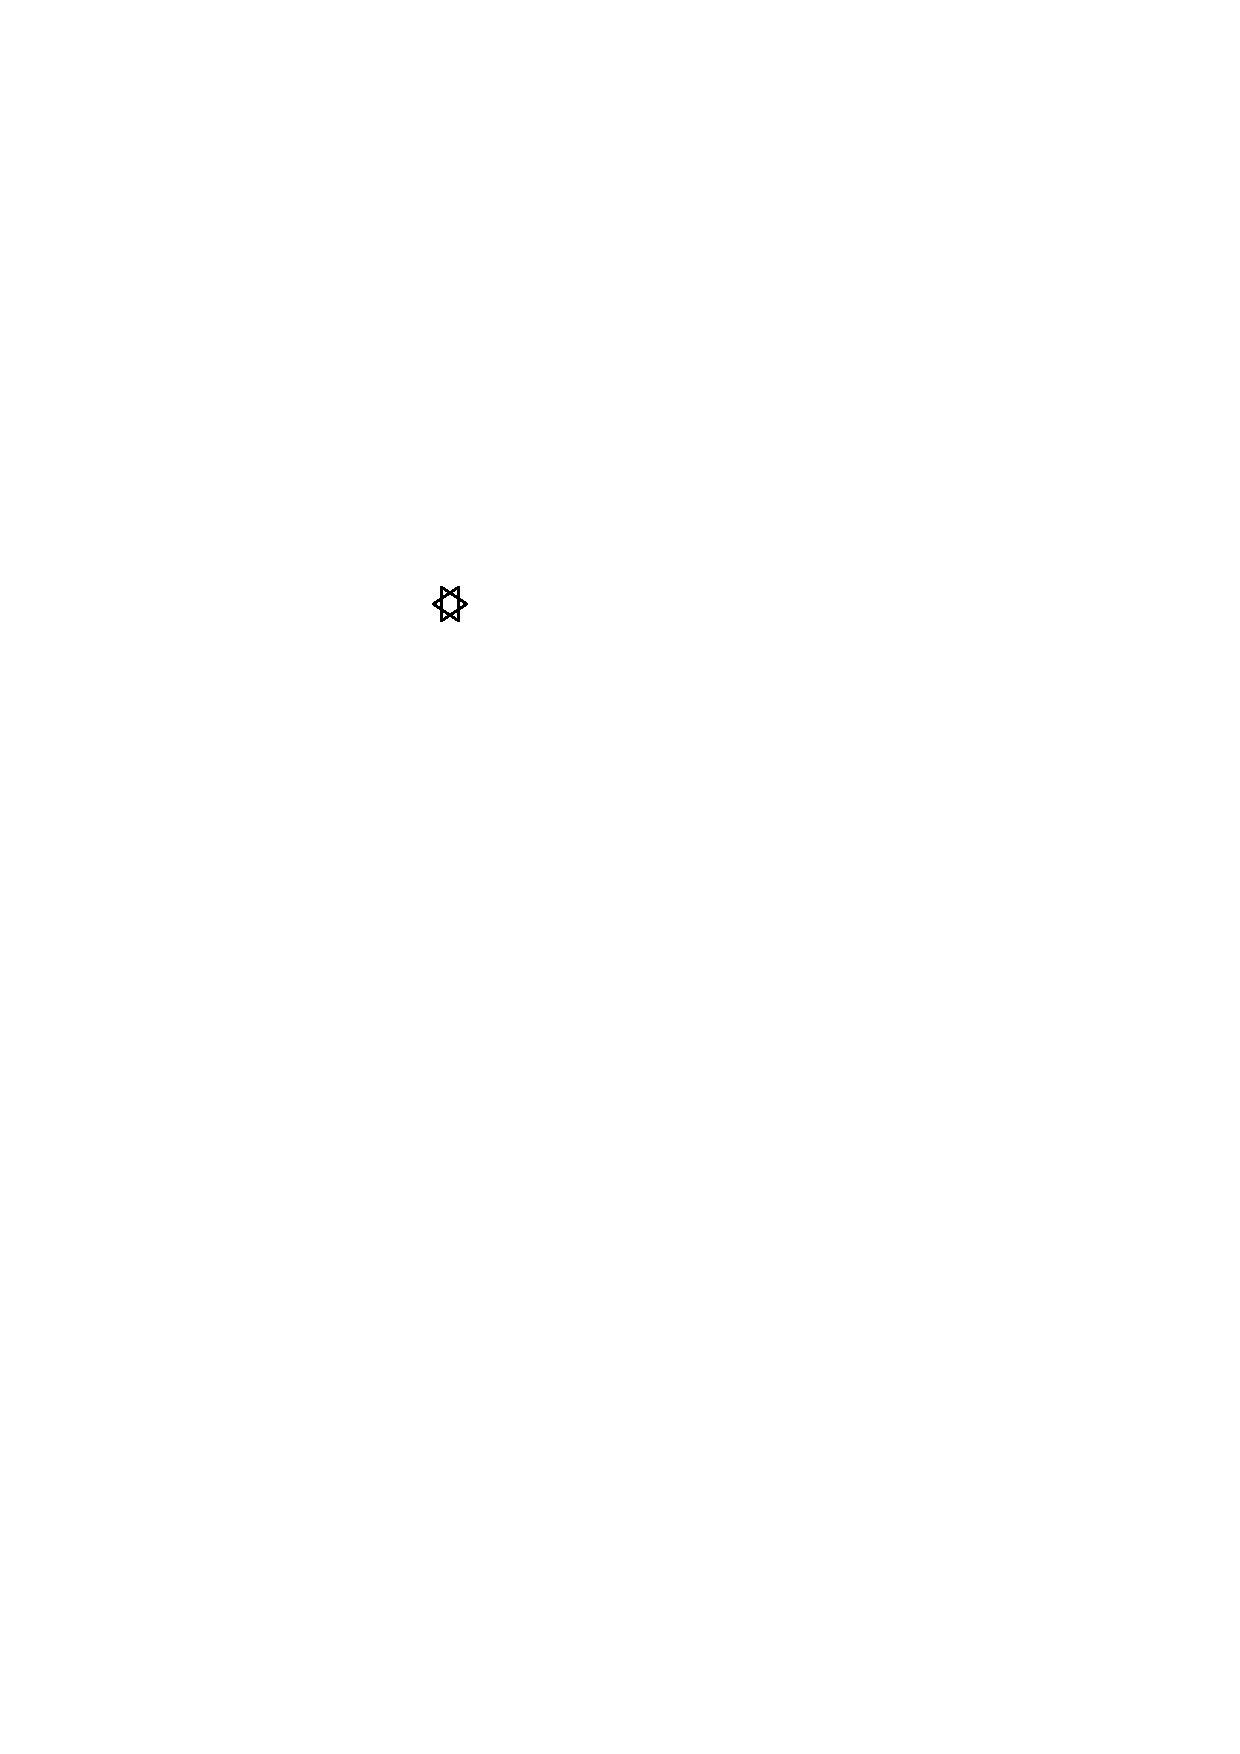
\includegraphics[height=1.6ex]{figs/triangles-disjoint-3}}}

\DeclareMathOperator{\ex}{ex}
\DeclareMathOperator{\on}{\overline{ex}}



%\usepackage{lineno}
%\linenumbers

\pagenumbering{roman}
\begin{document}
\begin{titlepage}
\maketitle

\begin{abstract}
  We study the following family of problems: Given a set of $n$ points
  in convex position, what is the maximum number triangles one can
  create having these points as vertices while avoiding certain sets
  of \emph{forbidden configurations}.  As forbidden configurations
  we consider all 8 ways in which a pair of triangles in such a point
  set can interact.  This leads to 256 extremal Turán-type questions.
  We give nearly tight (within a $\log n$ factor) bounds for 248 of these
  questions and show that the remaining 8 questions are all asymptotically
  equivalent to Stein's longstanding tripod packing problem.
\end{abstract}

\end{titlepage}

\tableofcontents

\newpage

\section{Introduction}
\pagenumbering{arabic}

Let $t_1$ and $t_2$ be a pair of distinct triangles whose (4--6) vertices
are in convex position.  There are 8 combinatorially distinct ways that
these triangles can interact:  2 ways in which the triangles can share
an edge (\taco\ and \mariposa), 3 ways in which the triangles can share a
single vertex (\bat, \nested, and \crossing), and 3 ways in which
the triangles can have no vertices in common (\ears, \swords,
and \david).  Because it is difficult to keep track of nameless entities, we assign a mnemonic to each configuration:

\begin{center}
  \begin{tabular}{|c|c|c|c|c|c|c|c|c}\hline
    \taco & \mariposa & \bat & \nested & \crossing & \ears & \swords & \david \\
    taco & mariposa & bat & nested & crossing & ears & swords & david  \\ \hline
  \end{tabular}
\end{center}

We consider the following class of problems:  Given a set, $X$,
of combinatorial configurations of pairs of triangles, what is the
largest set, $S$, of triangles one can create whose vertices are $n$
points in convex position, and such that no pair of triangles in $S$
forms a configuration in $X$.  We call the size of this set $\ex(n,X)$.
For example, 
\begin{equation}
    \ex(n,\{\taco,\nested,\crossing,\swords,\david\}) = n-2 \enspace .
\end{equation}
This is because the set $X=\{\taco,\nested,\crossing,\swords,\david\}$
forbids any form of crossings between the edges of triangles. Thus, the
maximum number of triangles we can have while avoiding $X$ is the number
of triangles in a triangulation of a convex $n$-gon, i.e., $n-2$. 

\subsection{Previous Work}

Since there are eight possible forbidden configurations, there are
$2^8=256$ sets, $X$ for which we can study $\ex(n,X)$.  Some of these sets
have been previously studied.  Bra\ss, Rote, and Swanepoel used bounds on
the set $X=\{\ears,\swords,\bat,\nested\}$ to solve an Erd\H{o}s problem
on the maximum number of maximum area/perimeter triangles determined
by a point set. Bra\ss\ \cite{brass:turan} later began a systematic
study in which he gave tight bounds for all singleton $X$ and all
pairs of configurations in which two triangles share a single vertex.
These previous results are listed in \tabref{previous}.

\begin{table}
\begin{center}
\begin{tabular}{m{.55\textwidth}m{.4\textwidth}}
  \hline
  \textbf{Result} & \textbf{Ref.} \\ \hline\hline
  $\ex(n,\{\mariposa\})\in \Theta(n^3)$ \newline
  $\ex(n,\{\taco\})\in \Theta(n^2)$ & \cite{brass:turan} \\
  \hline
  $\ex(n,\{\bat\})\in \Theta(n^3)$ \newline
  $\ex(n,\{\nested\})\in \Theta(n^2)$ \newline
  $\ex(n,\{\crossing\})\in \Theta(n^2)$ & \cite{brass:turan} \\
  \hline
  $\ex(n,\{\ears\})\in \Theta(n^3)$ \newline
  $\ex(n,\{\swords\})\in \Theta(n^2)$ \newline
  $\ex(n,\{\david\})\in \Theta(n^2)$ & \cite{brass:turan} \\
  \hline
  $\ex(n,\{\bat,\nested\})\in \Theta(n^2)$ \newline 
  $\ex(n,\{\nested,\crossing\})\in \Theta(n^2)$ \newline
  $\ex(n,\{\bat,\crossing\})\in \Theta(n^2)$ & \cite{brass:turan} \\
  \hline
  $\ex(n,\{\ears,\swords,\bat,\nested\}) = n$ \newline
  $\on(n,\{\taco,\mariposa,\david,\crossing\}) = n$
    & \cite{brass.rote.ea:triangles} \\
  \hline
  $\ex(n,\{\bat,\nested,\crossing\}) \in \Theta(n)$ \newline
  $\ex(n,\{\taco,\mariposa\}) \in \Theta(n^2)$ \newline 
  $\ex(n,\{\ears,\swords,\david\}) \in \Theta(n^2)$ & from hypergraphs \\ \hline
  \end{tabular}
\end{center}
\caption{Known results on $\ex(n,X)$ for different sets $X$.}
\tablabel{previous}
\end{table}

Of course, upper and lower bounds are inherited through the subset
relationship: $\ex(n,X) \le \ex(n,Y)$ for any $X\supseteq Y$.
\tabref{smalltable} shows the complete set of results we obtain when we
apply this exhaustively to the list of previous results.  Each entry in
this table presents the asymptotic behaviour of $\ex(n,X)$ for the set
$X$ obtained as the union of the row and column label.  Asymptotically
tight bounds are colored blue, and gaps between lower and upper bounds
are coloured red. Previous results imply 35 tight bounds for 256 of the
possible choices of $X$.  The configuration $\mariposa$ is ommitted from
the table since a simple argument (\lemref{xcup}) shows that its inclusion
in $X$ does not change $\ex(n,X)$ by more than a constant factor.

\begin{table}
  \begin{center}
    \input{oldbounds.tex}
  \end{center}
  \caption{Old bounds for $\ex(n,X)$.}
  \tablabel{smalltable}
\end{table}


%One
%of the results in this paper is that nearly the same bound holds even
%if we allow the $\swords$ and $\david$ configuration. In particular,
%our \thmref{blech} shows that $\ex(n,\{\taco,\nested,\crossing\}) \in
%O(n\log n)$.
%
%Sometimes it is more natural to describe the allowable configurations than the forbidden configurations. For this, we use the notation 
%\[
%   \on(n,X) = \ex(n,\{\taco,\mariposa,\bat,\nested,\crossing,
%                       \ears,\swords,\david\} \setminus X) \enspace .
%\]
%


%\begin{tabular}{llll}\hline
%  $\ex(n,\taco,\bat)$ & \multicolumn{2}{c}{$\Theta(n^2)$} & \thmref{taco-bat} \\
%  $\ex(n,\taco,\nested)$ & $\Omega(n^{1.549})$ & $O(n^2)$ & [various] \\
%  $\ex(n,\taco,\nested,\david)$ & $\Omega(n)$ & $O(n\log n)$ & \thmref{taco-nested-david} \\
%  $\ex(n,\taco,\crossing)$ & & & \\
%  $\ex(n,\taco,\ears)$ & \multicolumn{2}{c}{$\Theta(n^2)$} & \thmref{taco-ears} \\
%  $\ex(n,\taco,\david)$ & \multicolumn{2}{c}{$\Theta(n^2)$} & \thmref{taco-david} \\
%  $\ex(n,\taco,\swords)$ & $\Omega(n)$ & $O(n\log n)$ & \thmref{taco-swords} \\
%  $\ex(n,\bat,\nested)$ & \multicolumn{2}{c}{$\Theta(n^2$)} & \cite{brass:turan} \\
%  $\ex(n,\bat,\crossing)$ & \multicolumn{2}{c}{$\Theta(n^2$)} & \cite{brass:turan} \\
%  $\ex(n,\bat,\ears)$ & & & \\
%  $\ex(n,\bat,\swords)$ & \multicolumn{2}{c}{$\Theta(n^2$)} & \thmref{bat-swords} \\
%  $\ex(n,\bat,\david)$ & & & \\
%  $\ex(n,\nested,\crossing)$ & \multicolumn{2}{c}{$\Theta(n^2$)} & \cite{brass:turan} \\
%  $\ex(n,\nested,\ears)$ & & & \\
%  $\ex(n,\nested,\swords)$ & $\Omega(n)$ & $O(n\log n)$ & \thmref{nested-swords} \\
%  $\ex(n,\nested,\david)$ & & & \\
%  $\ex(n,\crossing,\ears)$ & & & \\
%  $\ex(n,\crossing,\swords)$ & $\Omega(n)$ & $O(n\log n)$ & \thmref{crossing-swords} \\$\ex(n,\crossing,\david)$ & & & \\
%  $\ex(n,\ears,\swords)$ & \multicolumn{2}{c}{$\Theta(n^2$)} & \thmref{swords-ears-david} \\
%  $\ex(n,\ears,\david)$ & \multicolumn{2}{c}{$\Theta(n^2$)} & \thmref{swords-ears-david} \\
%  $\ex(n,\swords,\david)$ & \multicolumn{2}{c}{$\Theta(n^2$)} & \thmref{swords-ears-david} \\
%\\ \hline
%\end{tabular}
%

\subsection{New Results}

In the current paper, we determine, up to a logarithmic factor, the
asymptotics of $\ex(n,X)$ for 248 sets $X$.  These results are shown in
\tabref{bigtable}. For the remaining 8 sets, we have determined that
the asymptotics are all the same and are equivalent to a problem that
appears in various contexts and under different names, including monotone
matrices, tripod packing, and 2-comparable triples. We discuss this
problem and its rich history in \secref{tripods}.  

\begin{table}
  \begin{center}
    \input{bounds.tex}
  \end{center}
  \caption{New and previous bounds for $\ex(n,X)$, up to a factor of $\log n$.
  For the new bounds listed as $n$, the lower bound is $\Omega(n)$ and the upper bound is $O(n\log n)$.  For the bounds listed as $n^{1.546}:n^2$, the upper bound is actually $n^2/e^{\Omega(\log^* n)}$.}
  \tablabel{bigtable}
\end{table}

The remainder of this paper is organized as follows.  In
\secref{points-of-view} we discuss different ways of thinking about
the problem and give some easy results.  In particular, we present a
series of puzzles whose solutions determine the asymptotic growth of
$\ex(n,X)$.  We then use this view to derive new upper and lower bounds
in \secref{new-results}.

\section{Points of View and Easy Results}
\seclabel{points-of-view}

In this section we present an easy result that cuts our work in half
by reducing the number of problems from 256 to 128.  We then describe
different variants of the problem, some of which are easier to work with.

\subsection{Edge-Sharing Non-Overlapping Triangles are Irrelevant}

The following lemma shows that including the $\mariposa$ configuration in
the set $X$ of forbidden configurations has no effect on the asymptotics
of $\ex(n,X)$.

\begin{lem}\lemlabel{xcup}
   For any $X$, $\ex(n,X\cup\{\mariposa\}) \ge \ex(n,X)/8$.
\end{lem}

\begin{proof}
  Let $S$ be a set of triangles that achieves $\ex(n,X)$. For each pair
  of vertices $u$ and $w$ independently and uniformly choose a direction
  $\overrightarrow{uw}$ or $\overleftarrow{uw}$.  We then obtain a set
  $S'\subseteq S$ by removing any triangle that has a directed edge for
  which the triangle is to the left of the edge.  Observe that the set
  $S'$ does not contain a $\mariposa$ configuration.

  For any particular triangle $t\in S$, the probability that $t\in S'$
  is exactly $1/8$ since each of $t$'s three edges must be directed
  clockwise and edge directions are chosen independently.  By linearity of
  expectation, $\E[|S'|]=|S|/8=\ex(n,X)/8$.  We conclude therefore that
  there exists some subset $S''\subseteq S$ of size least $\ex(n,X)/8$
  that does not contain a $\mariposa$ configuration.  The set $S''$ proves
  that $\ex(n,X\cup\{\mariposa\}) \ge \ex(n,X)/8$.
\end{proof}

\subsection{Cubic-Sized Sets of Pairwise Crossing Triangles}

\begin{thm}\thmlabel{pairwise-crossing}
   $\ex(n,\{\ears,\bat,\mariposa\})=\Omega(n^3)$
\end{thm}

\begin{proof}
  Partition the points of the convex $n$-gon into three contiguous
  sets, $A$, $B$, and $C$, each of size $\lfloor n/3\rfloor$ or
  $\lceil n/3\rceil$, as appropriate.  Consider the set, $S$, of all
  triangles having one vertex in each of $A$, $B$, and $C$. It is easy
  to check that any two triangles in $S$ have a pair of edges that
  cross, thus they do not form any of \ears, \bat, or \mariposa.
  Furthermore, $|S|\ge \lfloor n/3\rfloor^3=\Omega(n^3)$, so
  $\ex(n,\{\ears,\bat,\mariposa\})=\Omega(n^3)$.
\end{proof}


\subsection{Linear-Sized Sets Using only a Single Configuration}

Since it is not explicitly stated in previous work, and we need it to complete our table, we now observe that for any configuration $x\in\{\taco,\bat,\nested,\crossing,\ears,\swords,\david\}$, one can create a linear-sized set of triangles that avoids all configurations except $x$.

\begin{thm}
For any $X\subset\{\taco,\bat,\nested,\crossing,\ears,\swords,\david\}$,
$\ex'(n,X)\in \Omega(n)$.
\end{thm}

\begin{proof}
  Let $x\in\{\taco,\bat,\nested,\crossing,\ears,\swords,\david\}$ be
  a configuration not in $X$.  Label the vertices of our convex $n$-gon
  $1,\ldots,n$ in counterclockwise order.  Depending on the value of $x$,
  we use one of the following constructions:
 \begin{enumerate}
    \item For $x=\taco$ we use the set of triangles $\{(1,2,i):i\in\{3,\ldots,n\}\}$.
    \item For $x=\bat$ we use the set of triangles $\{(1,3i-1,3i-2): i\in\{1,\ldots,\lfloor n/3\rfloor \}$.
    \item For $x=\nested$ we use the set of triangles $\{(1,i,n+2-i): i\in\{2,\lfloor n/2\rfloor\}\}$.
    \item For $x=\crossing$ we use the set of triangles $\{(1,i,\lfloor n/2\rfloor+i): i\in\{2,\lfloor n/2\rfloor\}-1\}$.
    \item For $x=\ears$ we use the set of triangles $\{(3i-2,3-1,3i): i\in\{1,\lfloor n/3\rfloor\}\}$.
    \item For $x=\swords$ we use the set of triangles $\{(i,\lfloor n/2\rfloor+2i-2,\lfloor n/2\rfloor+2i-1): i\in\{1,\lfloor n/2\rfloor\}\}$.
    \item For $x=\david$ we use the set of triangles $\{(i,\lfloor n/3\rfloor+i,\lfloor 2n/3\rfloor+i): i\in\{1,\lfloor n/3\rfloor\}\}$.
 \end{enumerate}
 In each case, the size of the set is $\Omega(n)$ and it is
 straightforward to verify that each pair of triangles in the set forms
 the configuration $x$ and therefore avoids all configurations in $X$.
\end{proof}



\subsection{The Top/Bottom View}

It will be helpful to gain a sense of orientation by considering
a top/bottom variant of $\ex(n,X)$ that is defined as follows (see
\figref{top-bottom}).  Partition the vertices of a convex $n$-gon using
a horizontal line into a \emph{top half} of size $\lceil n/2\rceil$
and a \emph{bottom half} of size $\lfloor n/2\rfloor$.  We define
$\ex'(n,X)$ analogously to $\ex(n,X)$ except that we only count triangles
having one vertex in the bottom half and two vertices in the top half.
When studying $\ex'$, each triangle we count has a naturally defined
\emph{bottom vertex} in the bottom half and a \emph{left vertex} and
\emph{right vertex}, each in the top half.

\begin{figure}
  \begin{center}
    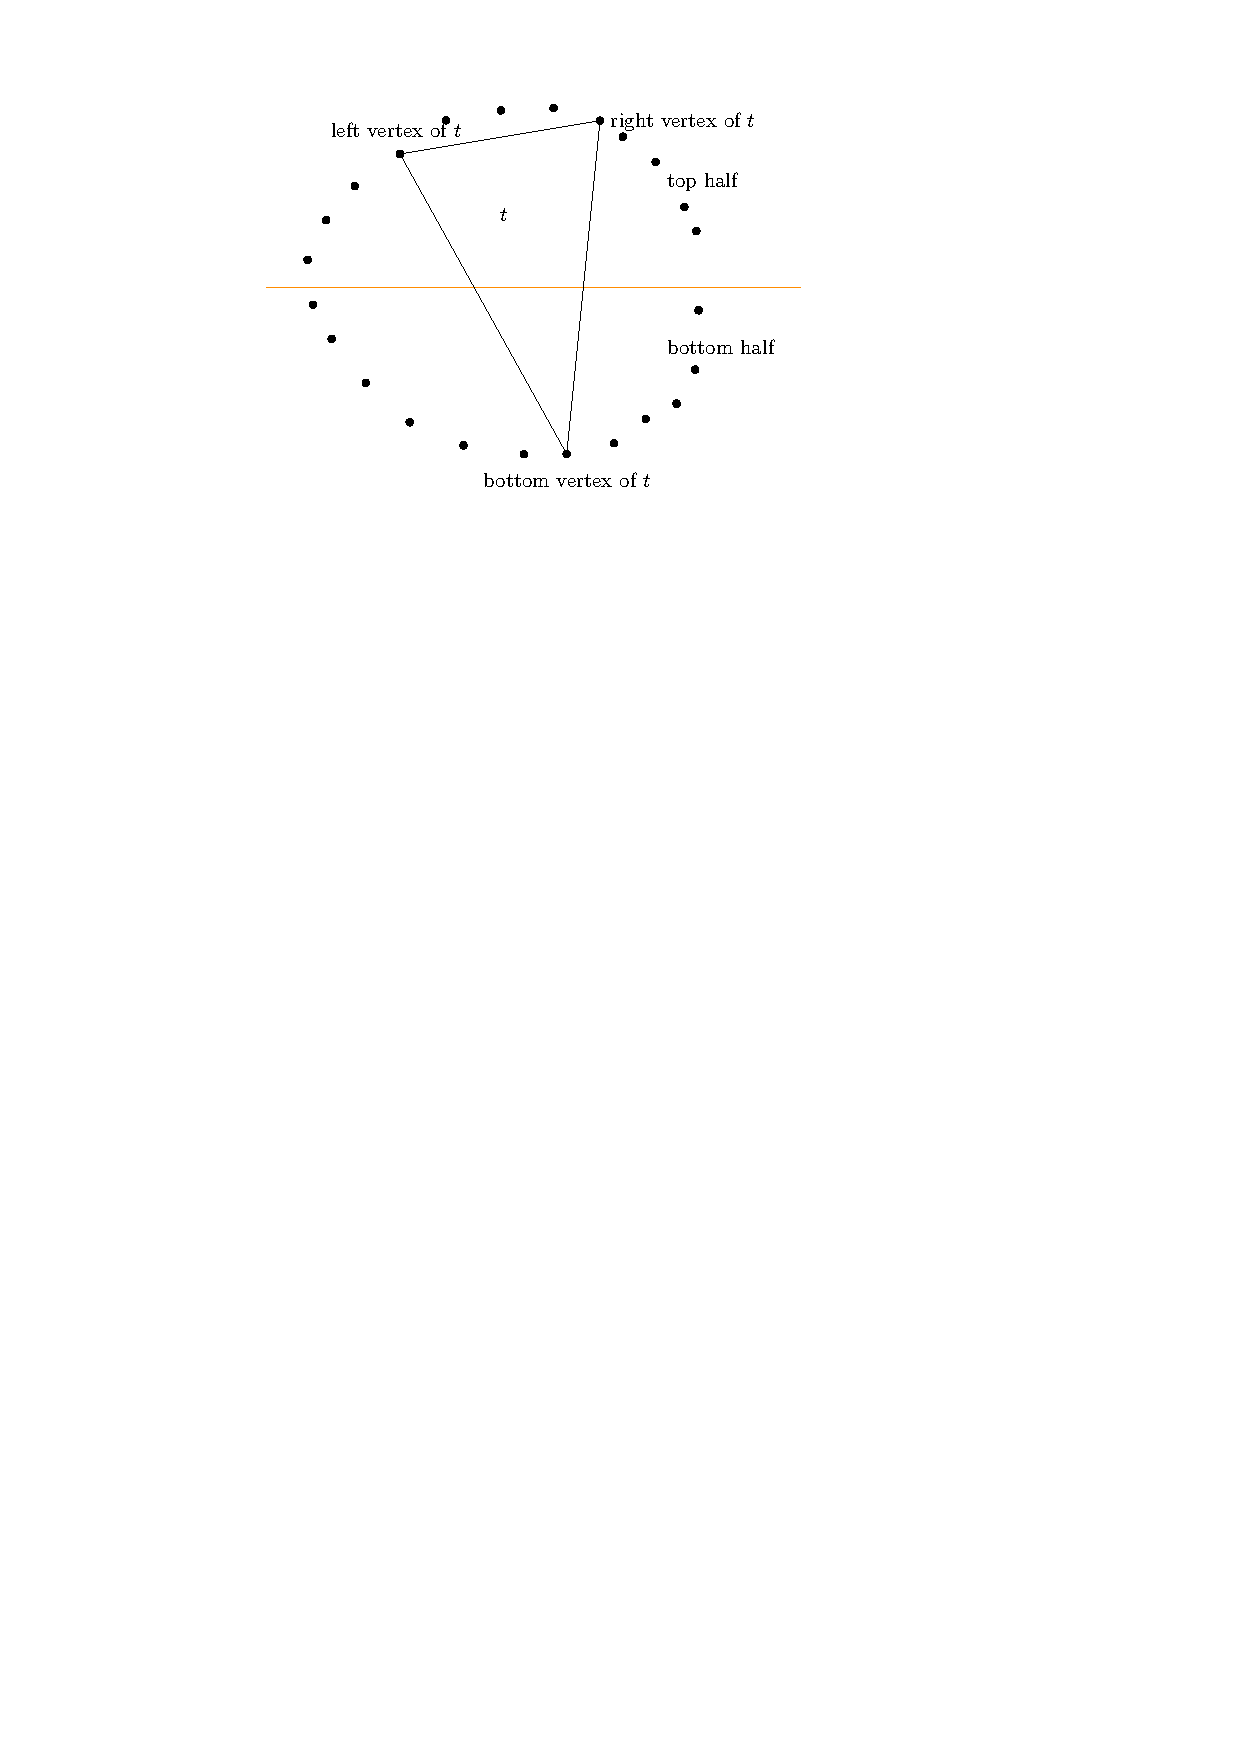
\includegraphics{figs/left-right}
  \end{center}
  \caption{$\ex'$ only counts triangles with two vertices in the top half
     and one vertex in the bottom half.}
  \figlabel{top-bottom}
\end{figure}

Clearly $\ex(n,X)\ge\ex'(n,X)$.  The following lemma shows that, without
losing much precision, we can also upper bound $\ex(n,X)$ by $\ex'(n,X)$.

\begin{lem}\lemlabel{top-bottom}
  If $\ex'(n,X)\in O(n^c)$, then
  \[
     \ex(n,X)\in 
        \begin{cases} 
            O(n^c)     & \text{if $c>1$} \\
            O(n\log n) & \text{if $c=1$}
        \end{cases}
  \]
\end{lem}

\begin{proof}
   Let $S$ be a set of triangles that avoids $X$.  Every triangle in $S$
   is of one of the following types:
   \begin{enumerate}
      \item It has one vertex in the top half and two in the bottom half;
        there are $O(n^{c})$ such triangles.
      \item It has two vertices in the top half and one in the bottom
        half; there are $O(n^{c})$ such triangles.
      \item It has all three vertices in the top half; there are at most
        $\ex(\lceil n/2\rceil,X)$ such triangles.
      \item It has all three vertices in the bottom half; there are at
        most $\ex(\lfloor n/2\rfloor,X)$ such triangles.
   \end{enumerate}
   Thus, we obtain the recurrence inequality:
   \[  \ex(n,X) \le O(n^{c}) + \ex(\lceil n/2\rceil,X) + \ex(\lfloor n/2\rfloor,X) \]
   which resolves to $O(n^c)$ for $c>1$ and $O(n\log n)$ for $c=1$.
\end{proof}


\subsection{The Dot-Puzzle View}

The top-bottom version of the problem gives us a sense of orientation,
but it is still difficult to visualize the sets of triangles obtained
this way. Next, we show that there is a corresponding puzzle that is
easy to visualize.  Refer to \figref{point-view}.  

In this puzzle, we are given $\binom{n}{2}$ points,
\[
    Q = \{(x,y): y\in\{1,\ldots,n-1\}, x\in\{y+1,\ldots,n\} \} \enspace .
\]
These points model the top/bottom view on a convex $2n$-gon, where the
point $(x,y)$ represents a triangle whose vertices are some point on
the bottom and the $x$th and $y$th points on the top, where the top
vertices are labelled $1,\ldots,n$ from left to right.

\begin{figure}
   \begin{center}
      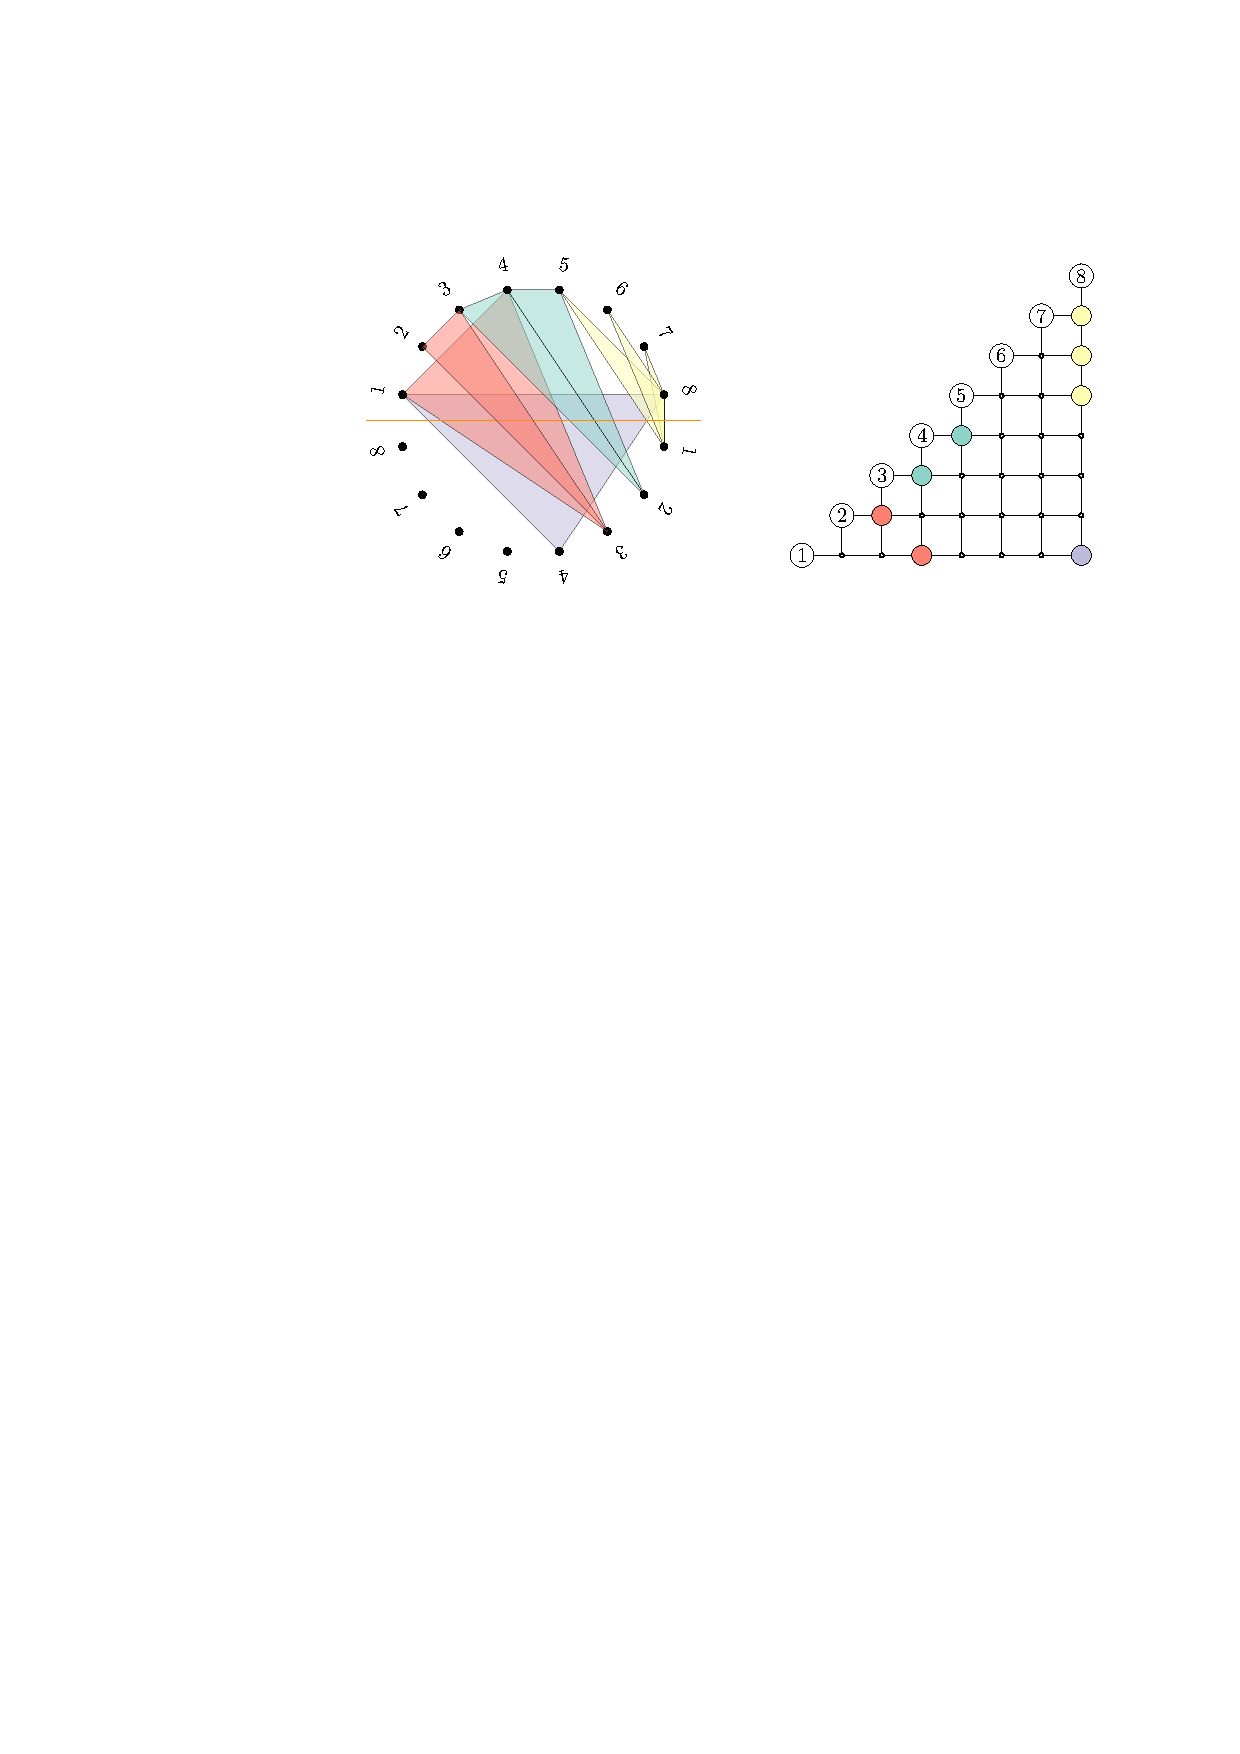
\includegraphics{figs/point-view}
   \end{center}
   \caption{The Dot-Puzzle View of the Top/Bottom View. In this example,
     four rounds of the Dot-Puzzle have been played.}
   \figlabel{point-view}
\end{figure}

The dot-puzzle proceeds in $n$ rounds and during the $i$th round, the
player selects a set $Q_i\subseteq Q$ subject to certain constraints
that depend on the points selected in rounds $1,\ldots,i-1$.  In the
top/bottom view, the $i$th round determines which pairs of top vertices
form a triangle with the $i$th bottom vertex, where the bottom
vertices are labelled $1,\ldots,n$ from right to left.  

Of course, the constraints on which points can be selected during
round $i$ depend on the set of forbidden configurations and the set
$\bigcup_{j=1}^{i-1} Q_i$ of points played during previous rounds.
By proving bounds on $\sum_{i=1}^n |Q_i|$ we obtain bounds on the maximum
number of triangles obtained in the top-bottom view on a set of $2n$
points.

\Figref{forbidden-color}.a shows restrictions on the locations of points
placed during a single round.  It is interpreted as follows:  If the
central point, $p=(x,y)$, is placed during round $i$, and we wish to
avoid some particular configuration, $c$, then we should not place any
points in the parts of the figure that are have label $c$.  For instance,
if we wish to avoid the configuration $c=\taco$ configuration, then we
should not place any points in the same row or column as $p$; such a point
creates a $\taco$ configuration in which the shared edge
joins a bottom vertex to a left (same row) or right (same column) vertex.

\Figref{forbidden-color}.b shows the constraints placed on the locations
of points placed in subsequent rounds.  Its interpretation is similar
\figref{forbidden-color}.a. For example, if we wish to avoid a
$\nested$ configuration and we place the central point, $p$, during round
$i$, then, in every round $j>i$, we should not place any point directly
to the left or directly below $p$.  Any such point creates 
a $\nested$ configuration in which the shared vertex is the left vertex
(to the left of $p$) or the right vertex (below $p$) of both triangles.

%One caveat worth noting is that, unless $\taco$ is a forbidden
%configuration, the same point can be chosen in different rounds.

%\begin{table}
%\begin{center}
%\begin{tabular}{m{1ex}|>{\centering\arraybackslash}m{.45\textwidth}|>{\centering\arraybackslash}m{.45\textwidth}}
%      & killed by $(x,y)$ in later rounds 
%         & killed by $(x,y)$ in current round \\ \hline
%$\mariposa$ & 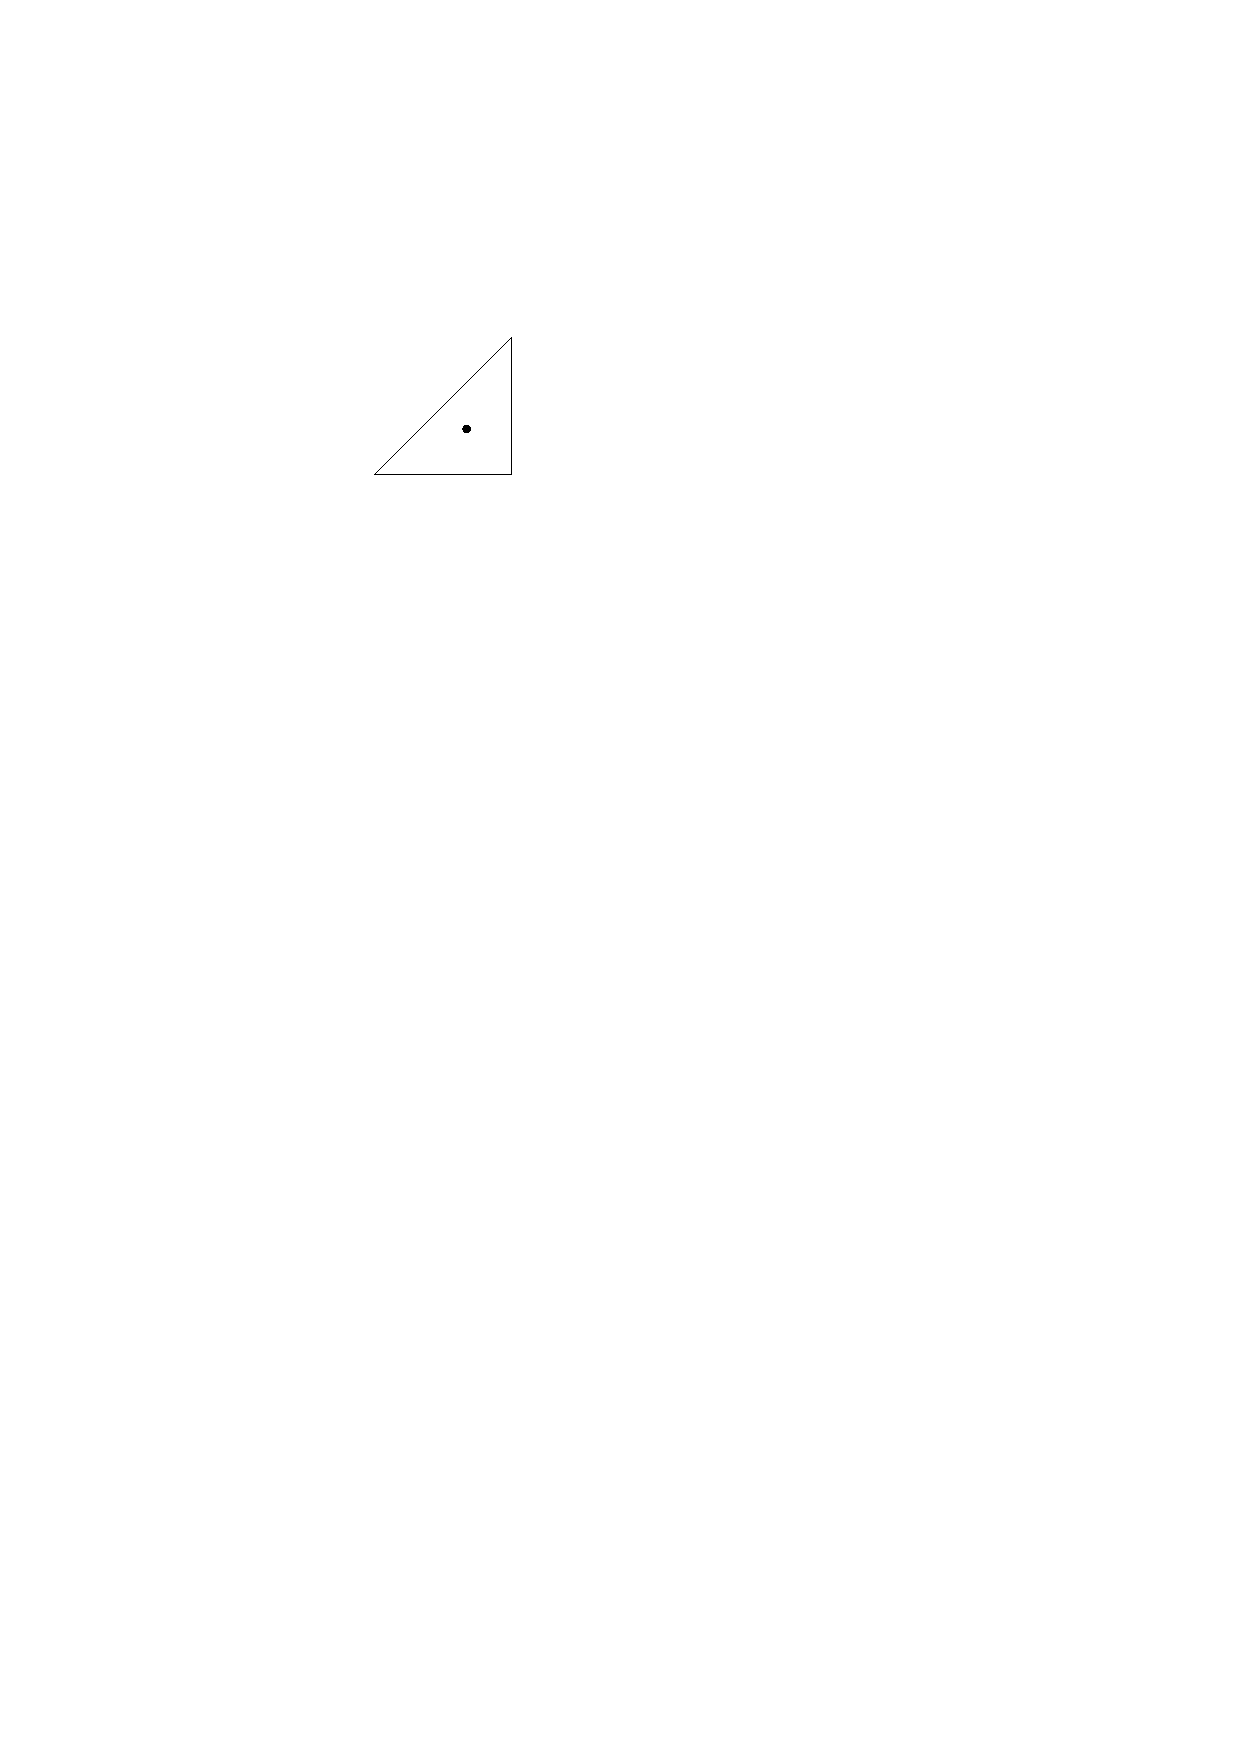
\includegraphics[scale=.8]{figs/killers-1} \break% 
%           $\{\}$  
%         & 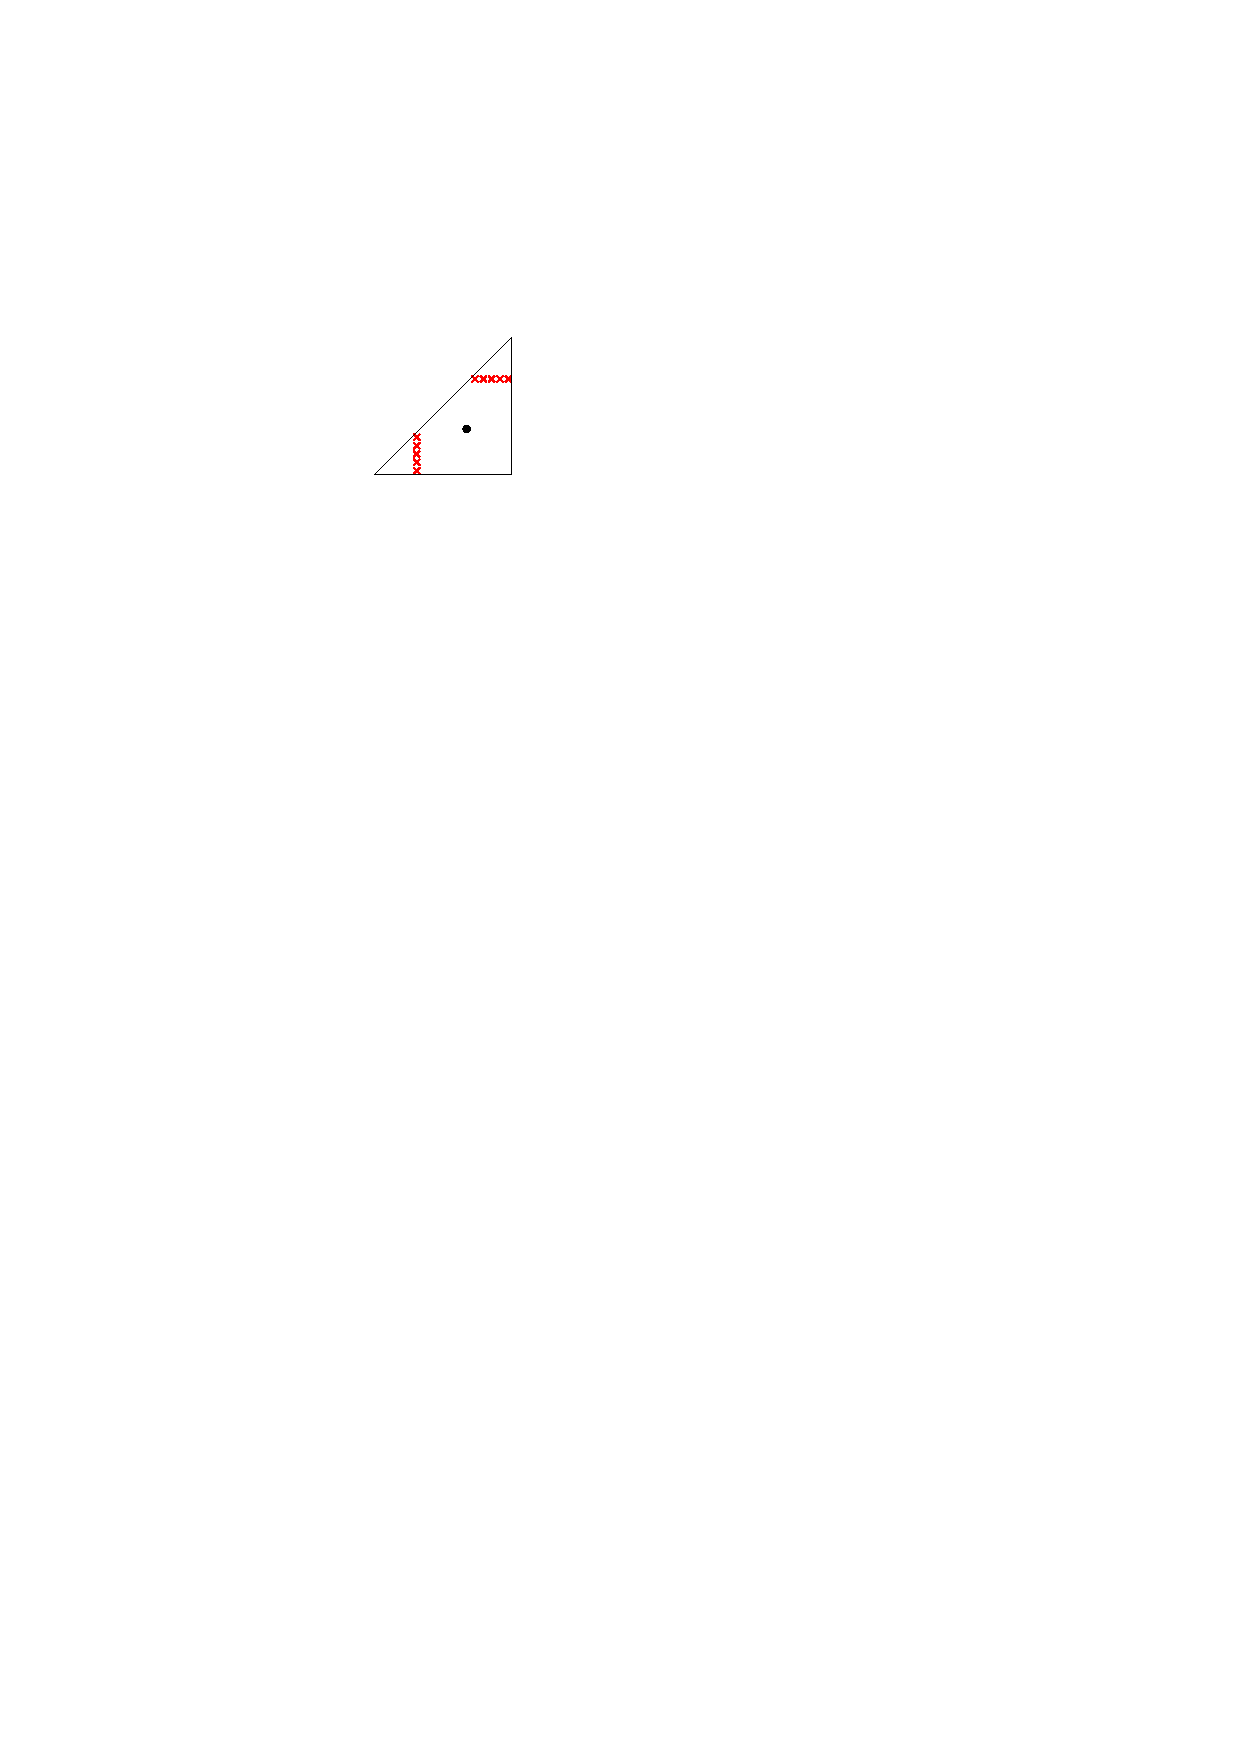
\includegraphics[scale=.8]{figs/killersb-1} \break% 
%           $\{(x',x)\} \cup \{(y,y')\}$ \\ 
%$\taco$ & 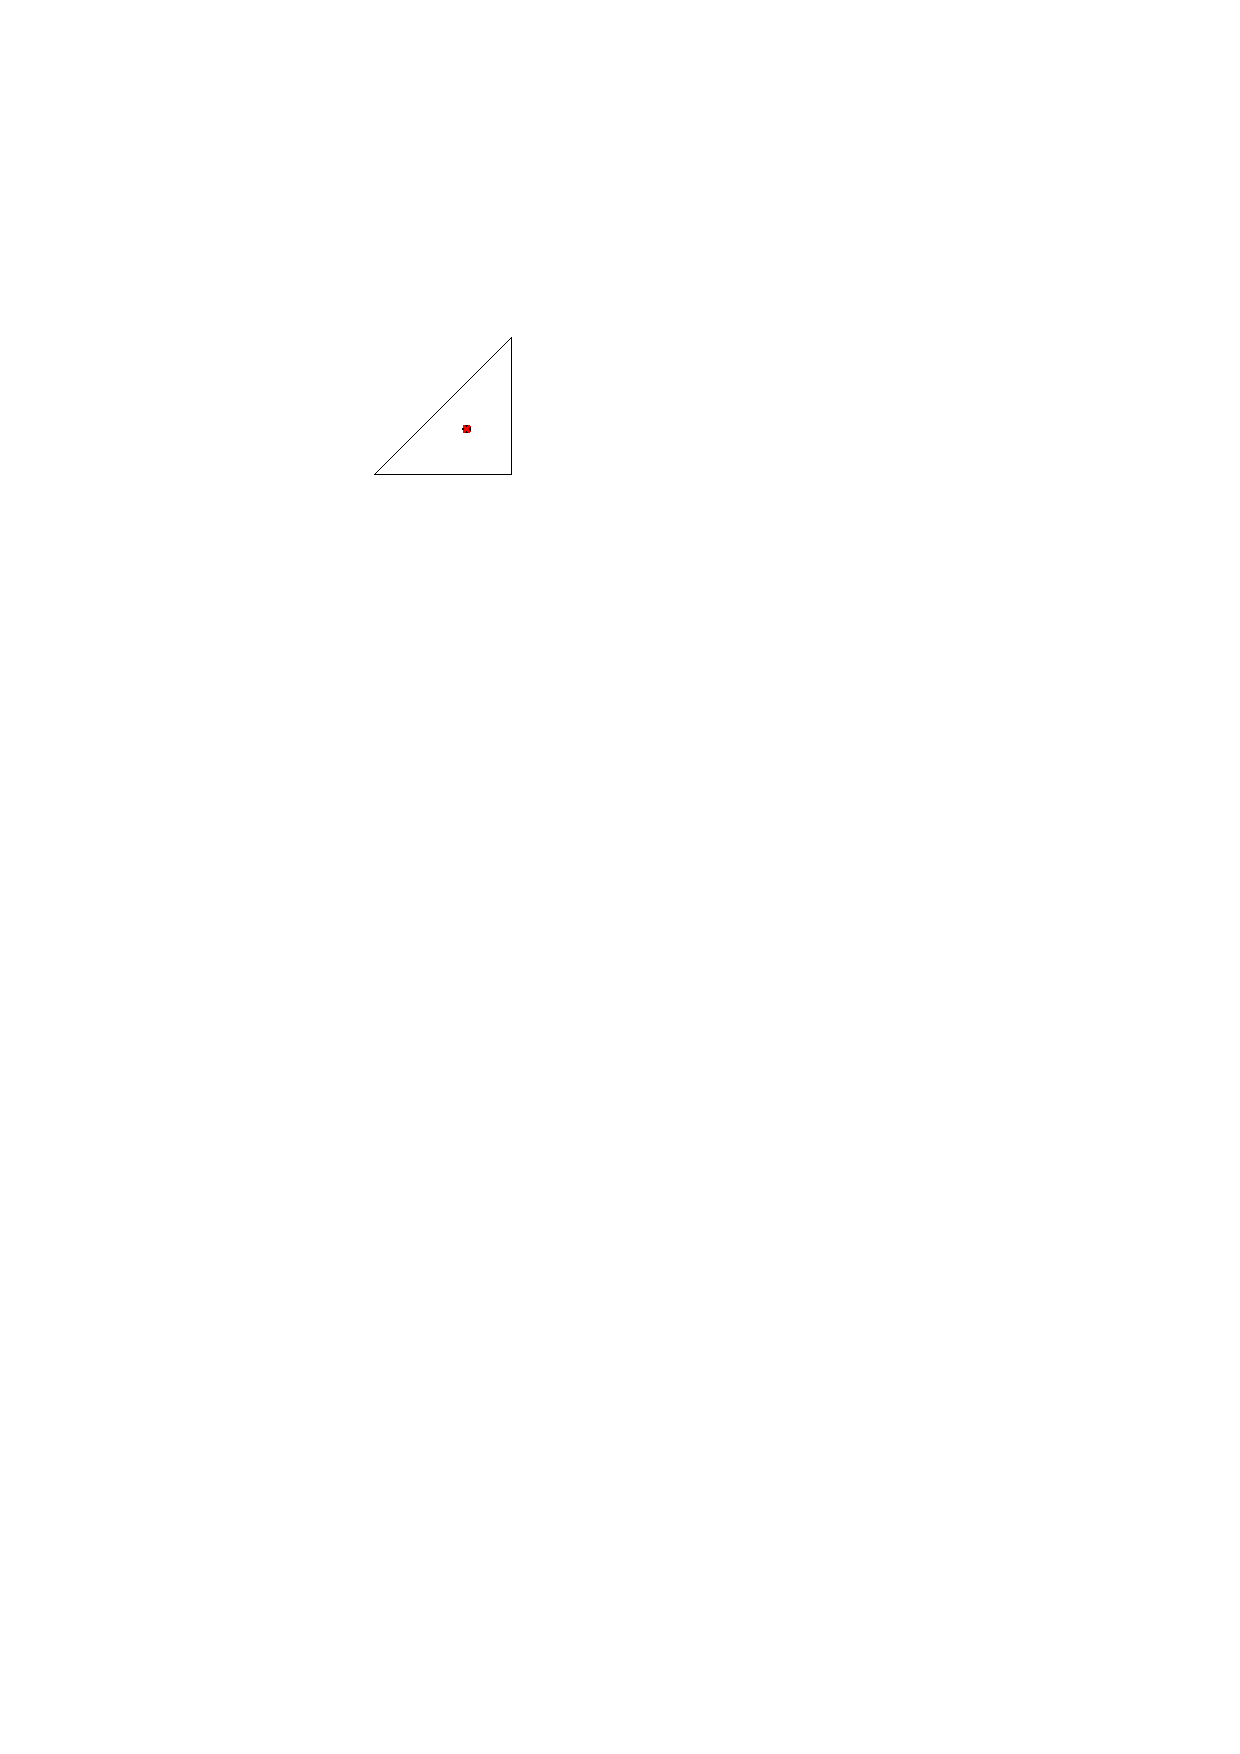
\includegraphics[scale=.8]{figs/killers-2} \break% 
%           $\{(x,y)\}$ 
%         & 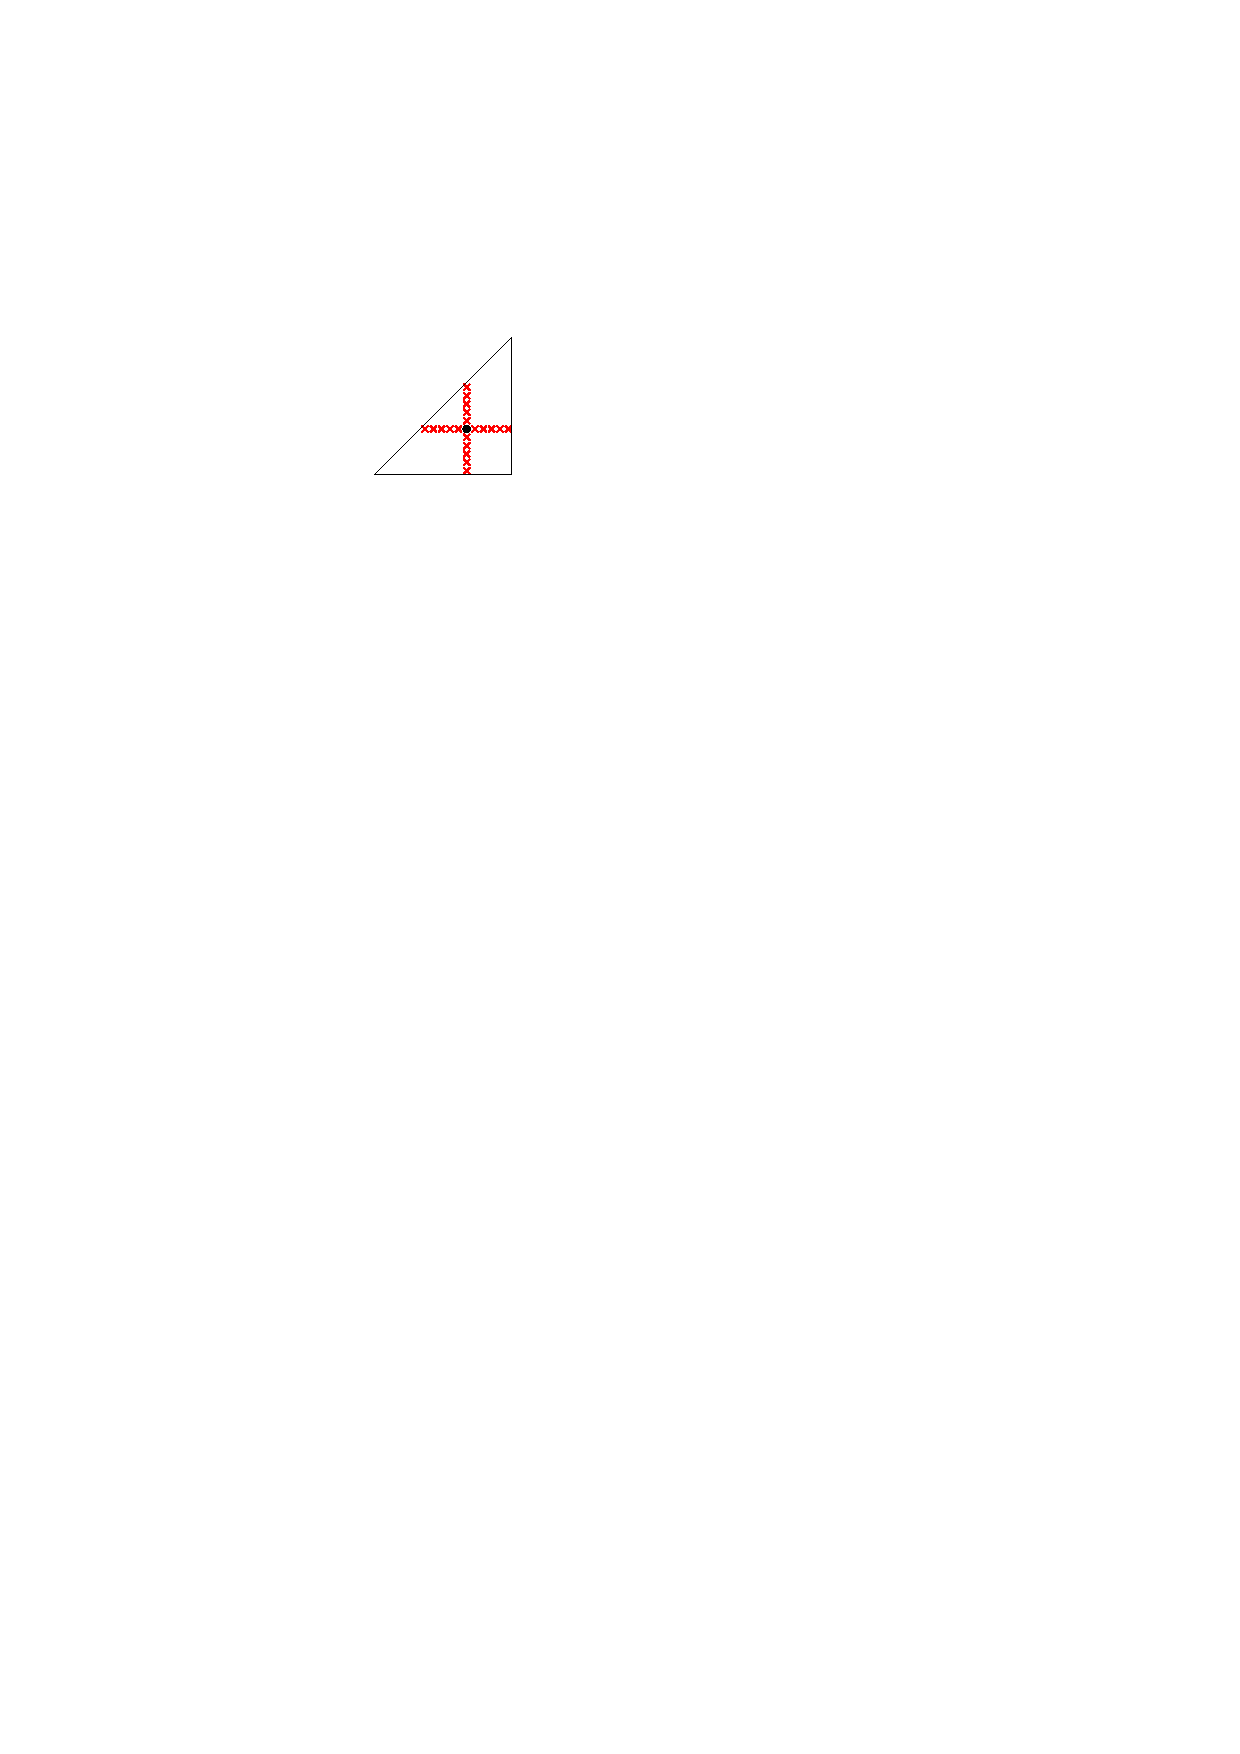
\includegraphics[scale=.8]{figs/killersb-2} \break% 
%           $\{(x,y')\} \cup \{(x',y)\}$ \\
%$\bat$ & 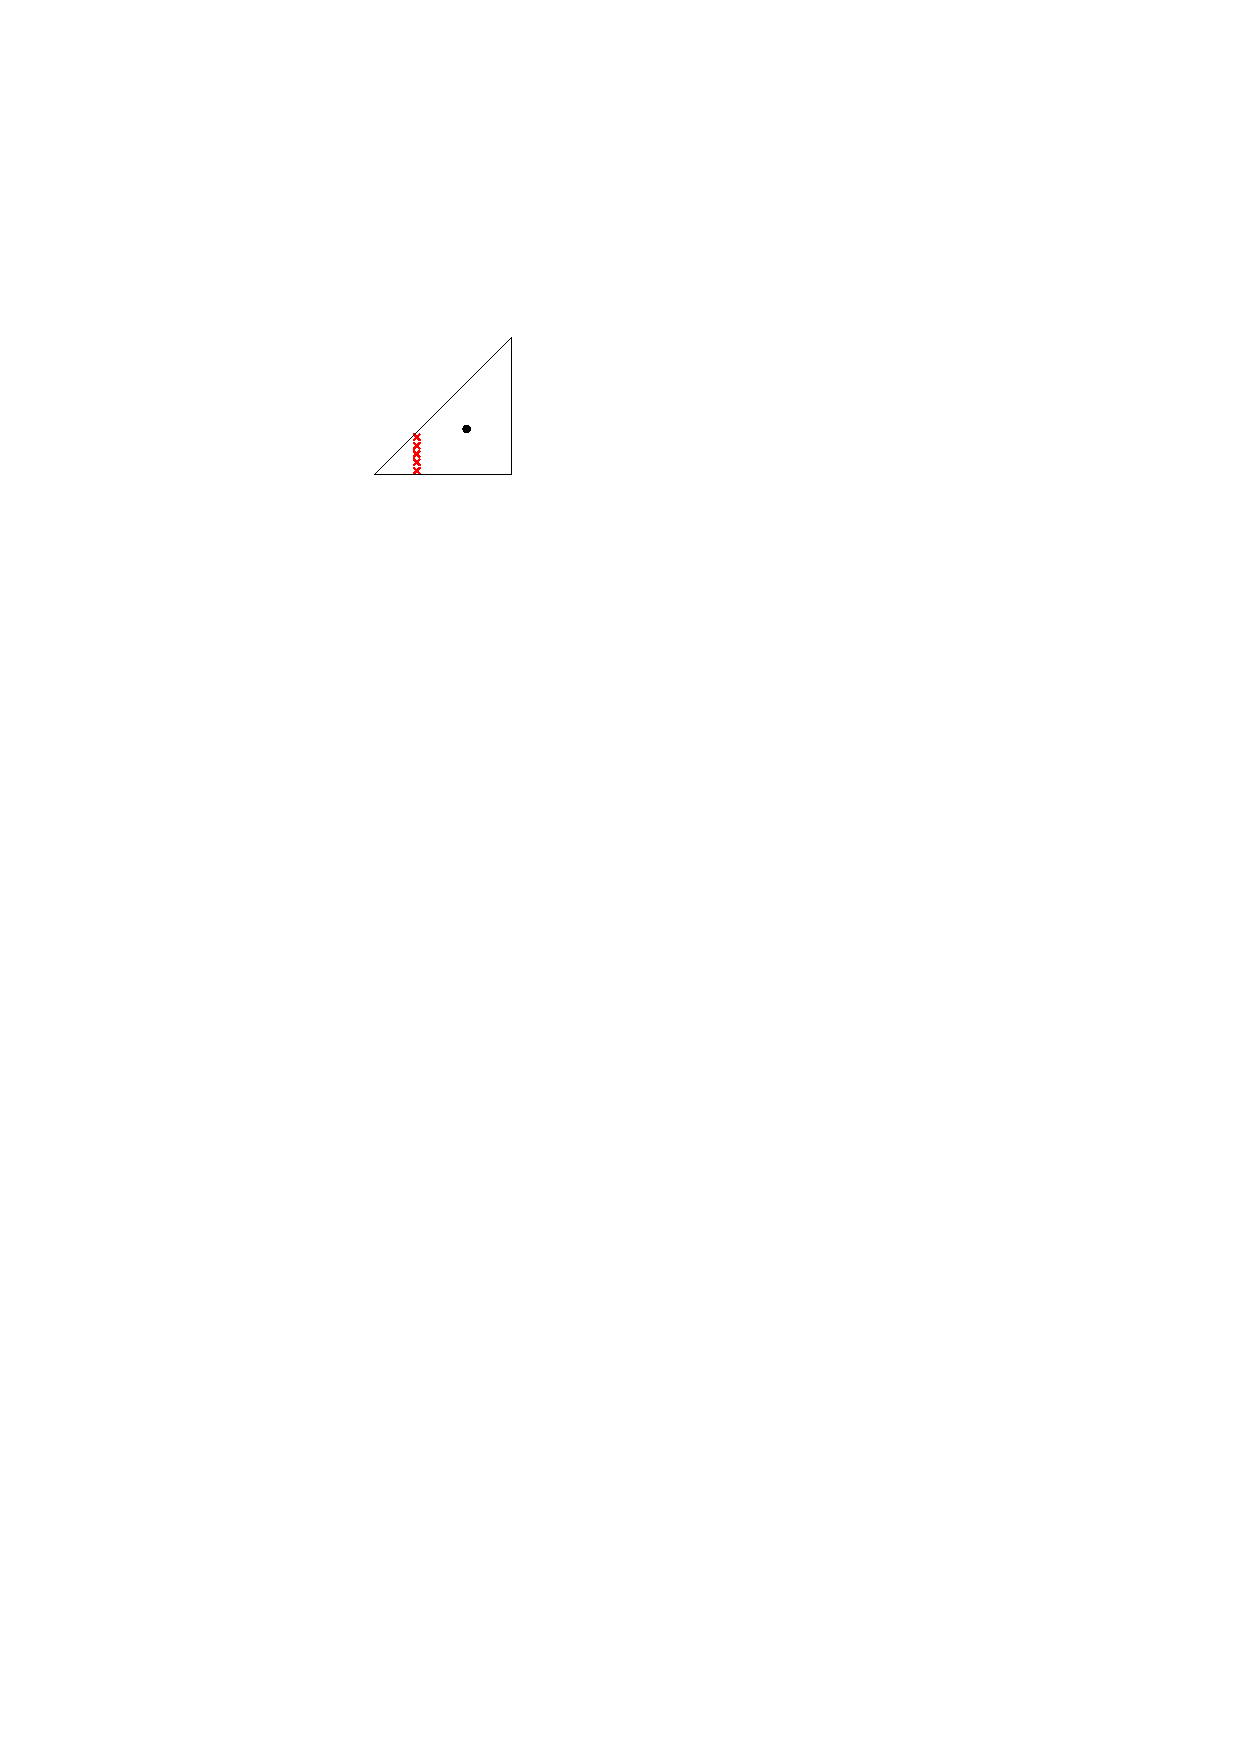
\includegraphics[scale=.8]{figs/killers-3} \break% 
%             $\{(x',y) : x'<x \}\cup\{(x,y') : y'<y \}$ 
%           & 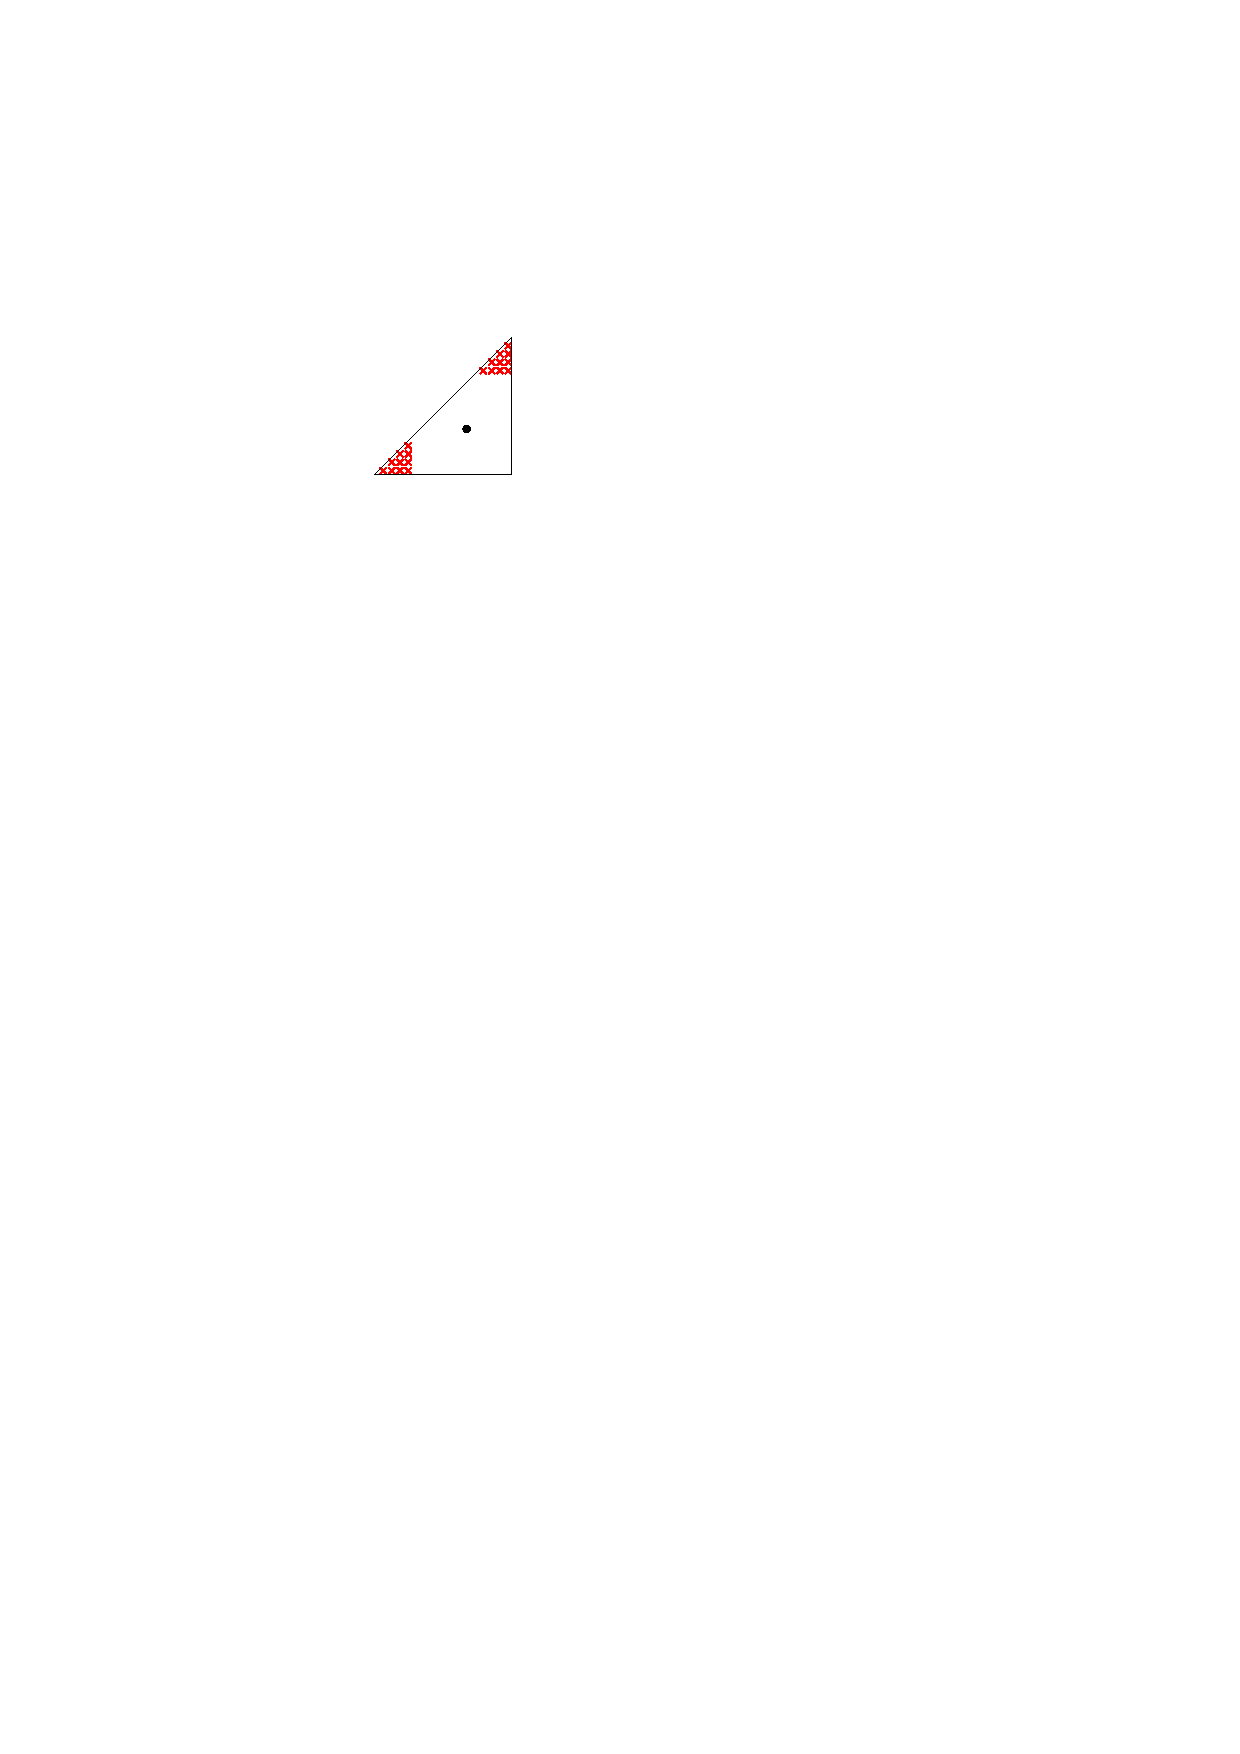
\includegraphics[scale=.8]{figs/killersb-3} \break%
%             $\{(x',y'): x' < y\text{ or } y'> x\}$ \\
%$\nested$ &  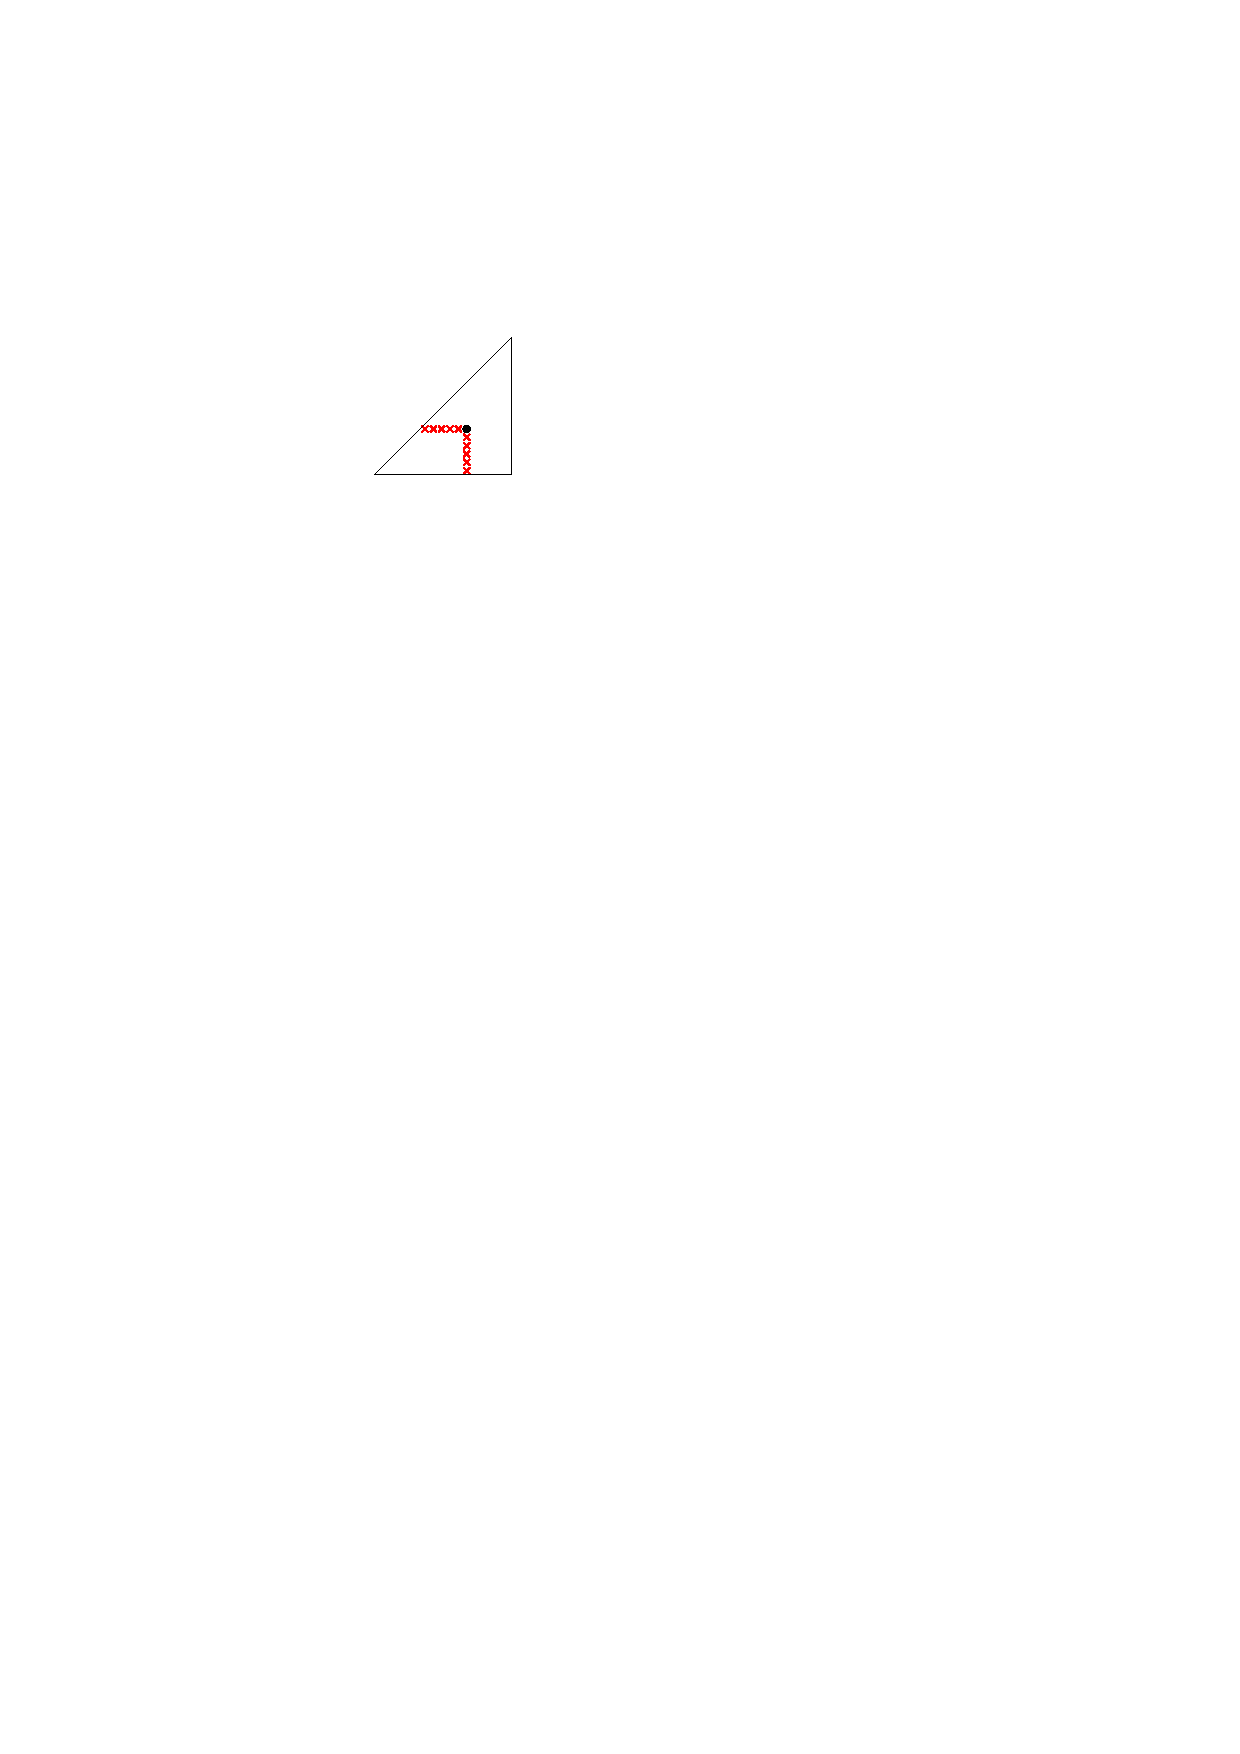
\includegraphics[scale=.8]{figs/killers-4} \break%
%              $\{(x',y) : x'<x \}\cup\{(x,y') : y'<y \}$ 
%         &  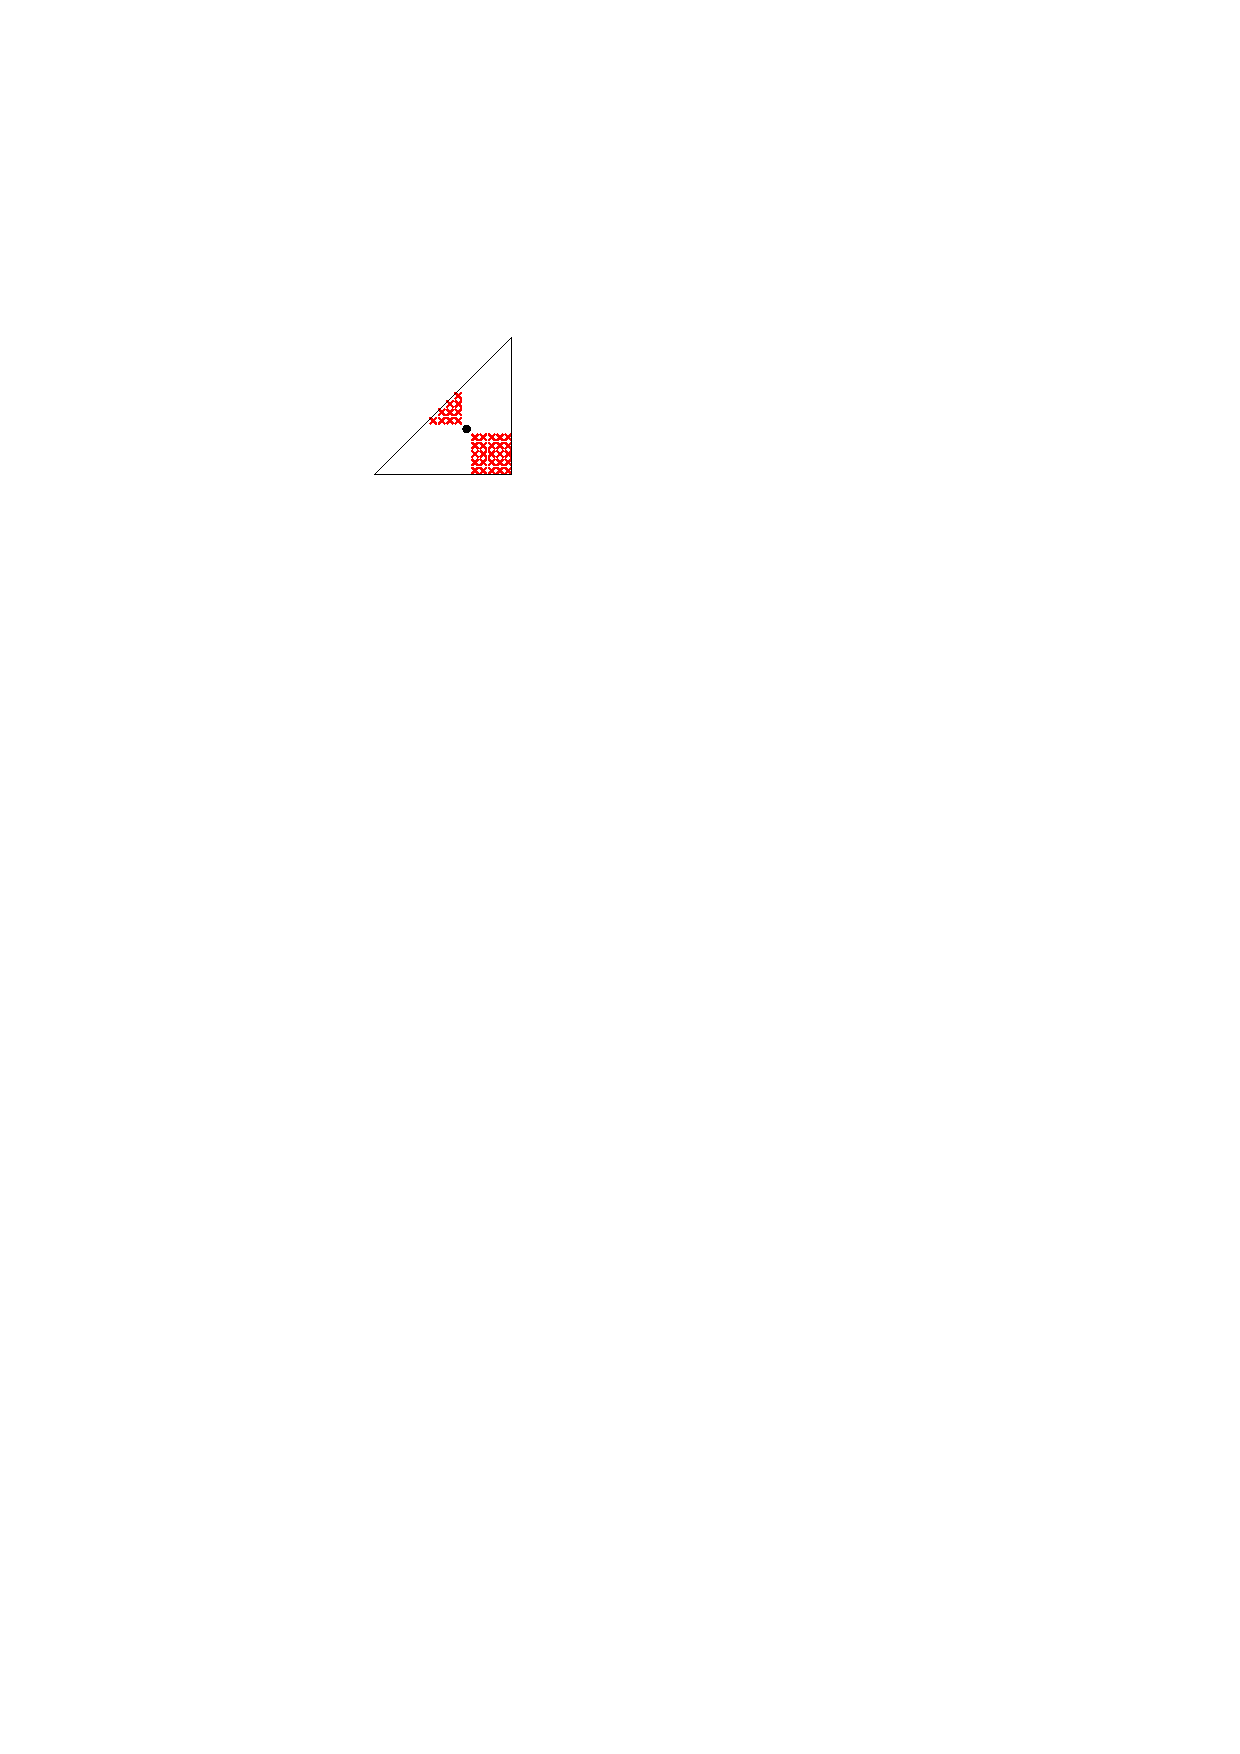
\includegraphics[scale=.8]{figs/killersb-4} \break%
%            $\{(x',y'):\sign(x'-x)=\sign(y-y')\}$ \\
%$\crossing$ &  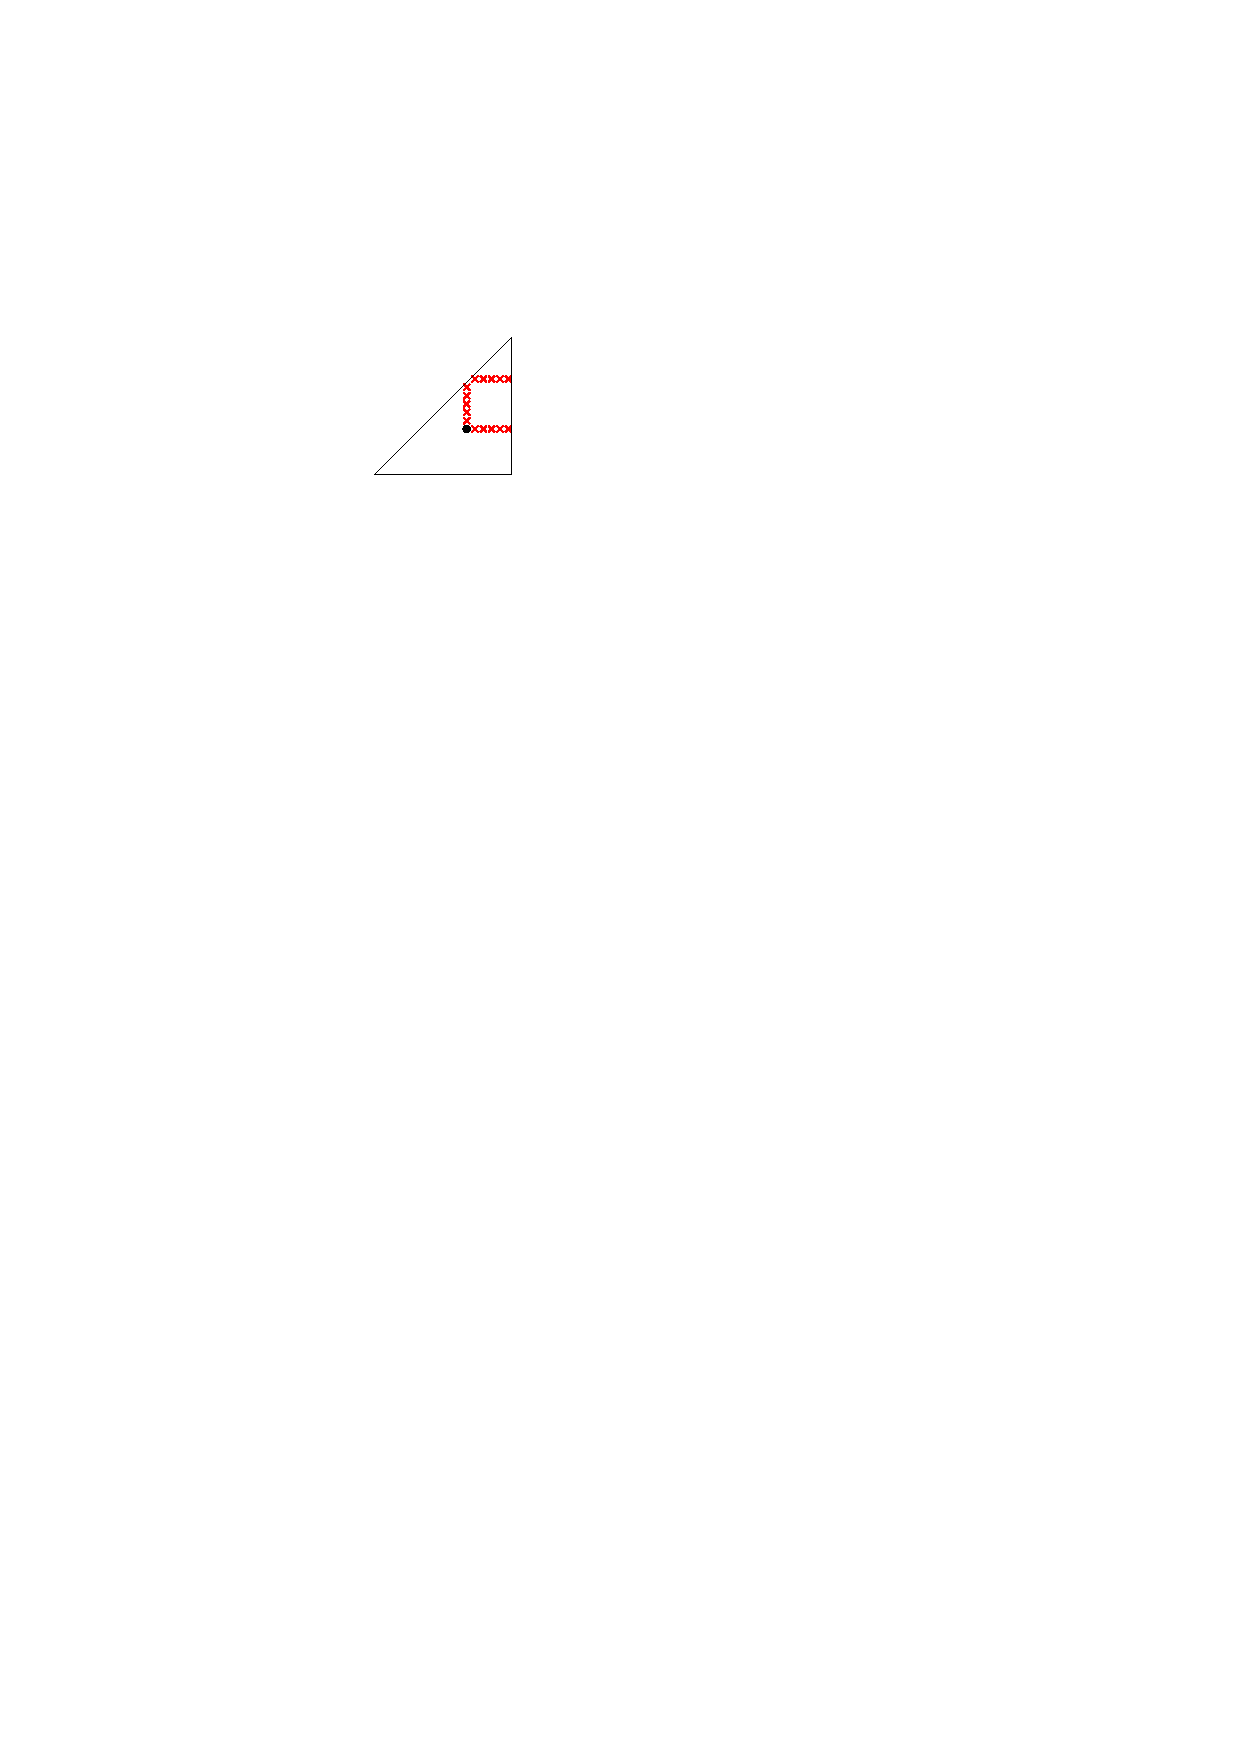
\includegraphics[scale=.8]{figs/killers-5} \break% 
%              $\{(x',y) : x'>x \}\cup\{(x,y') : y'>y \}$ 
%         &  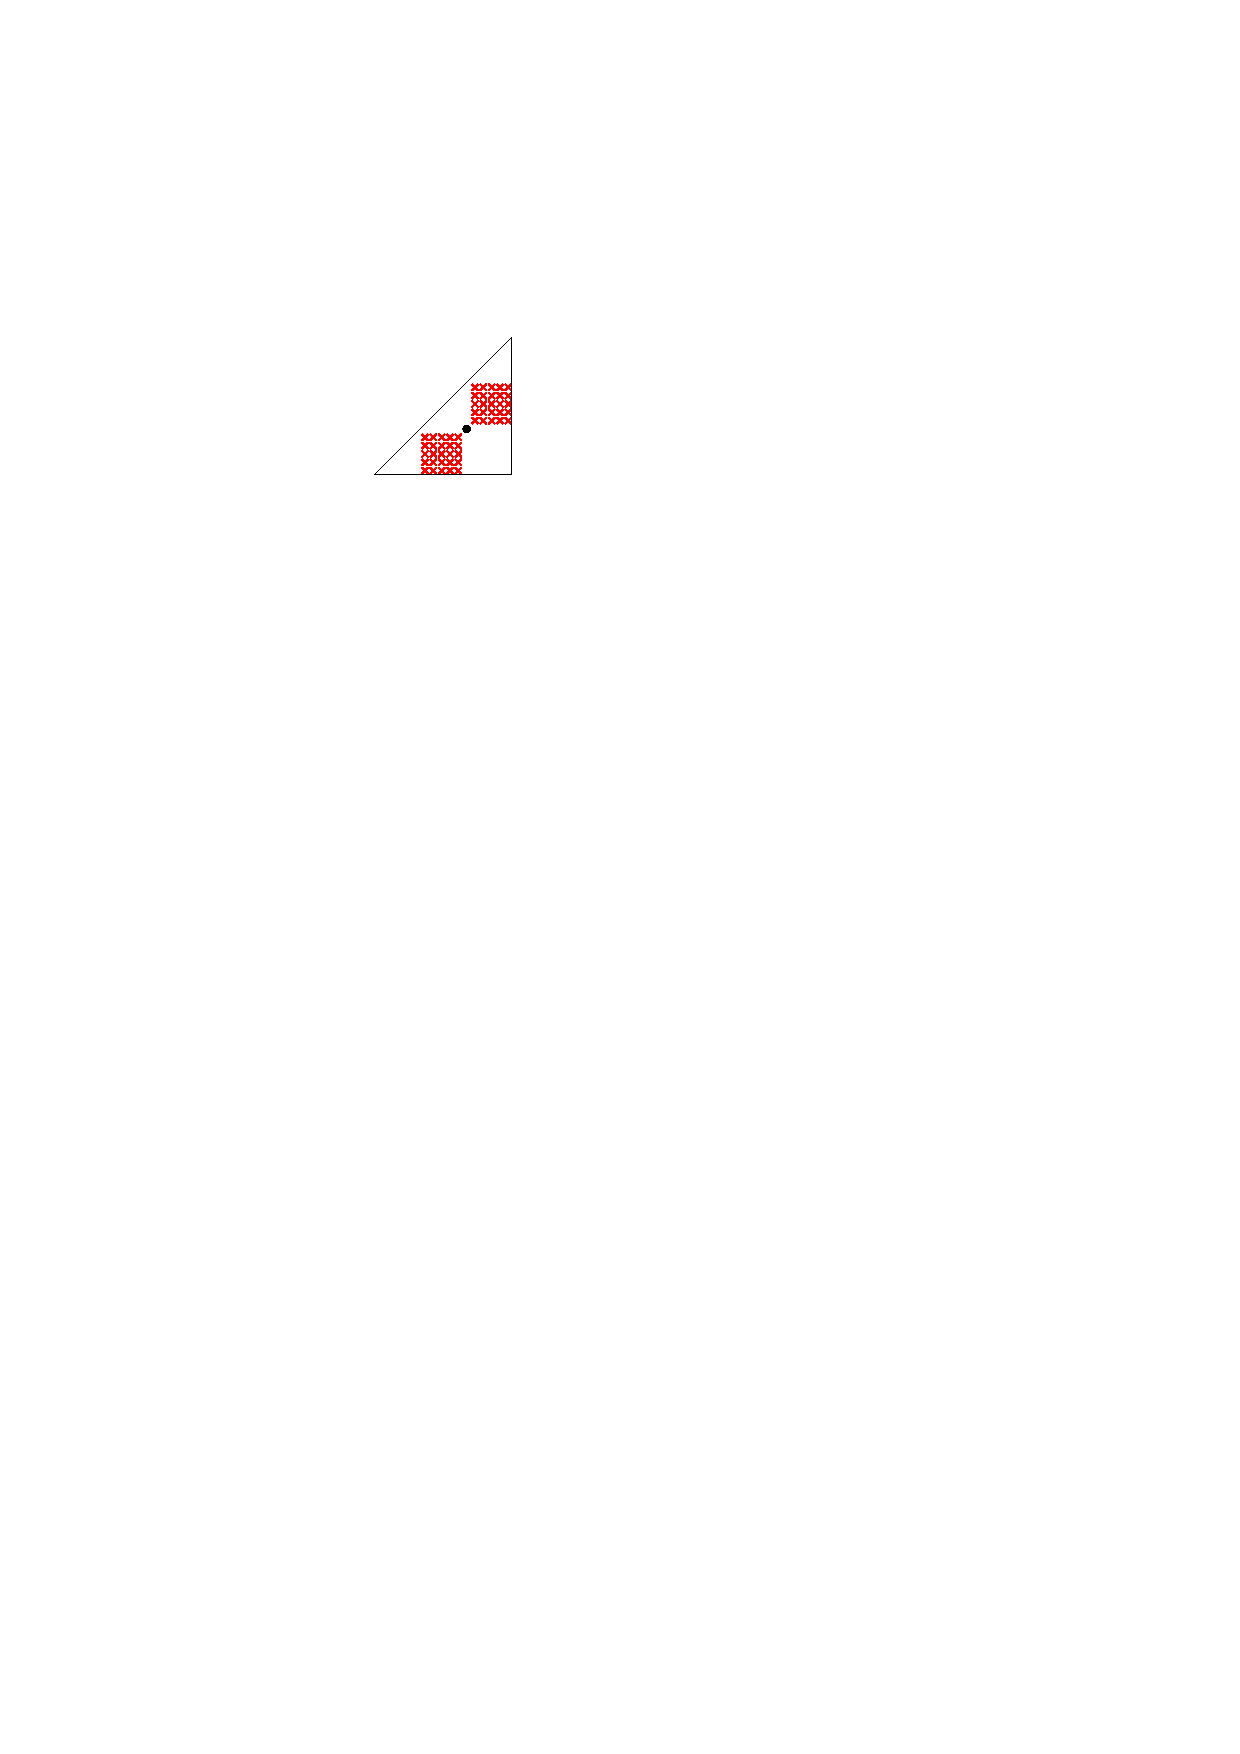
\includegraphics[scale=.8]{figs/killersb-5} \break% 
%            $\{(x',y'):\sign(x'-x)=\sign(y'-y)\}$ \\
%$\ears$ &  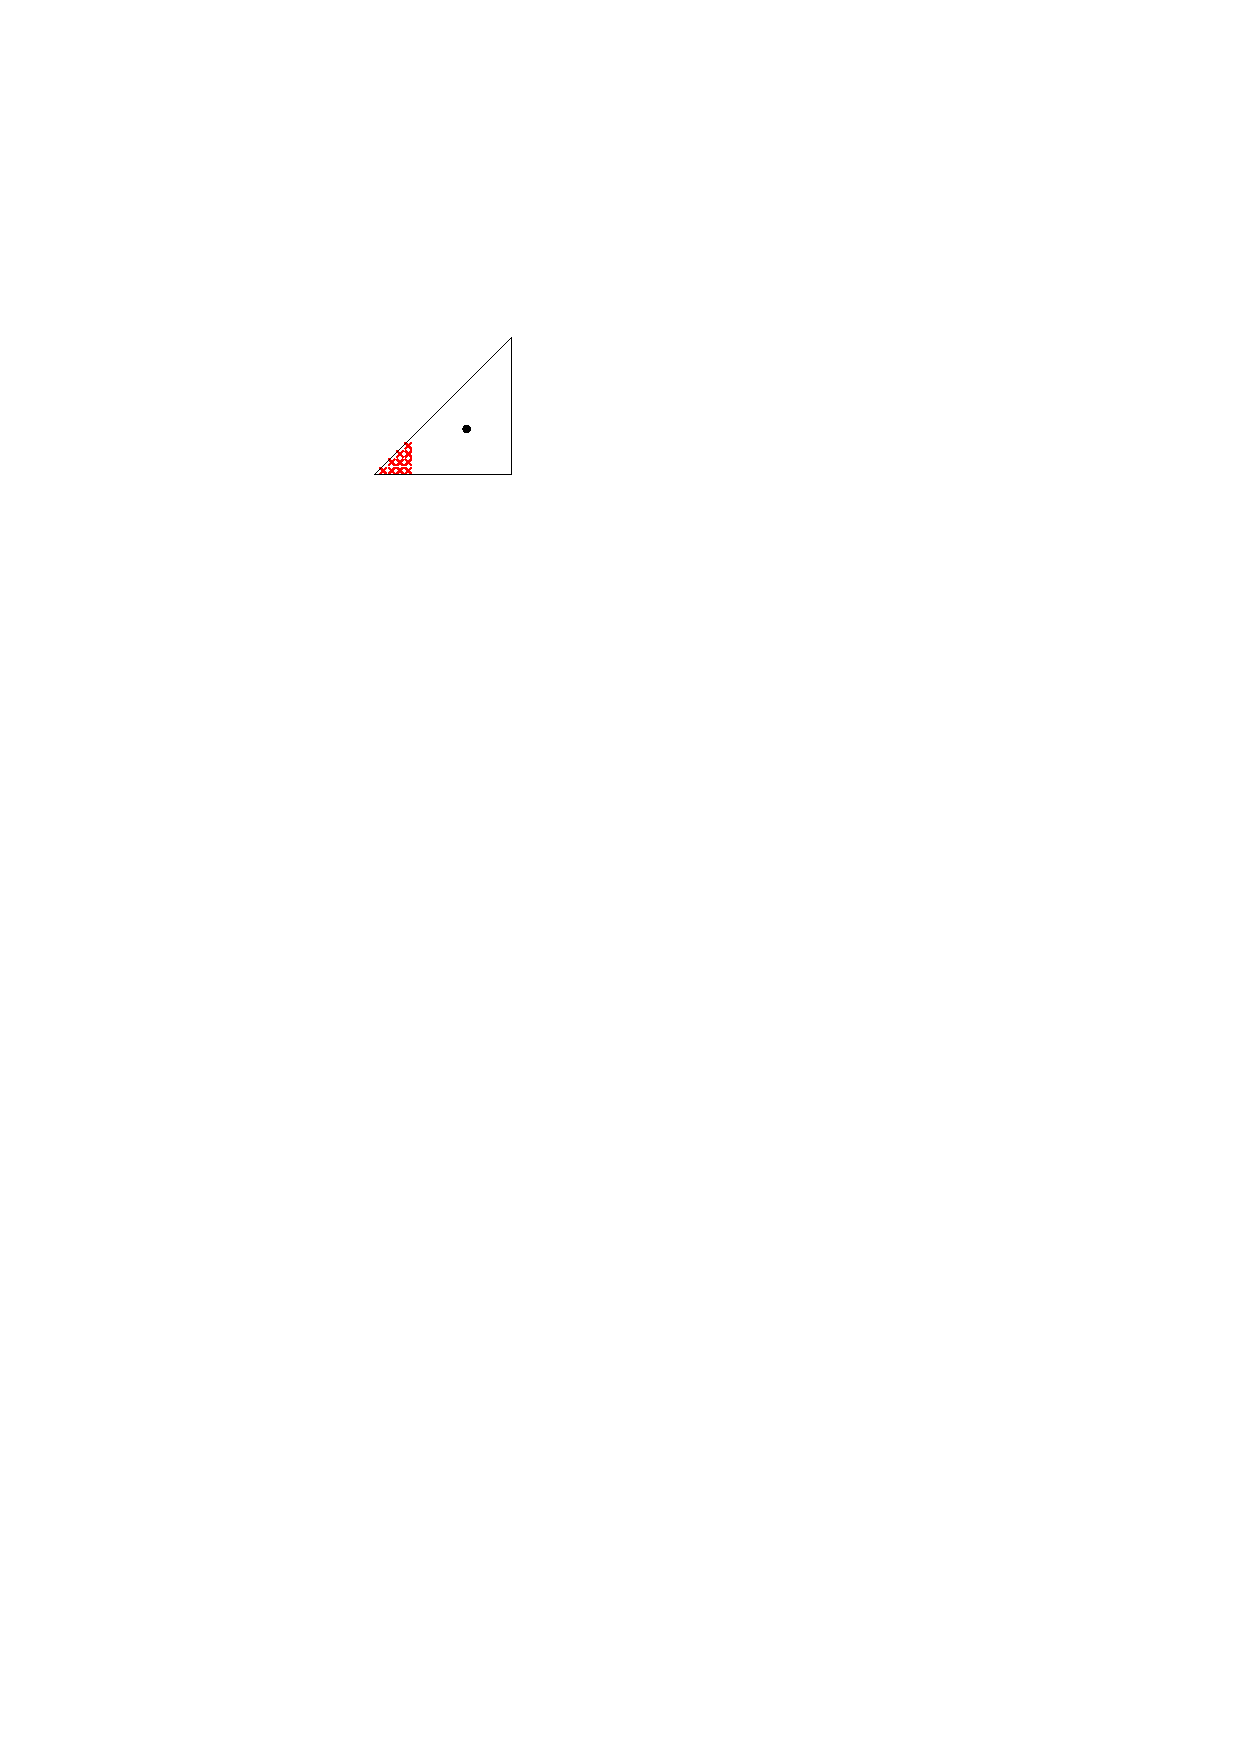
\includegraphics[scale=.8]{figs/killers-6} \break%
%                $\{(x',y'): x'< y\}$
%         & 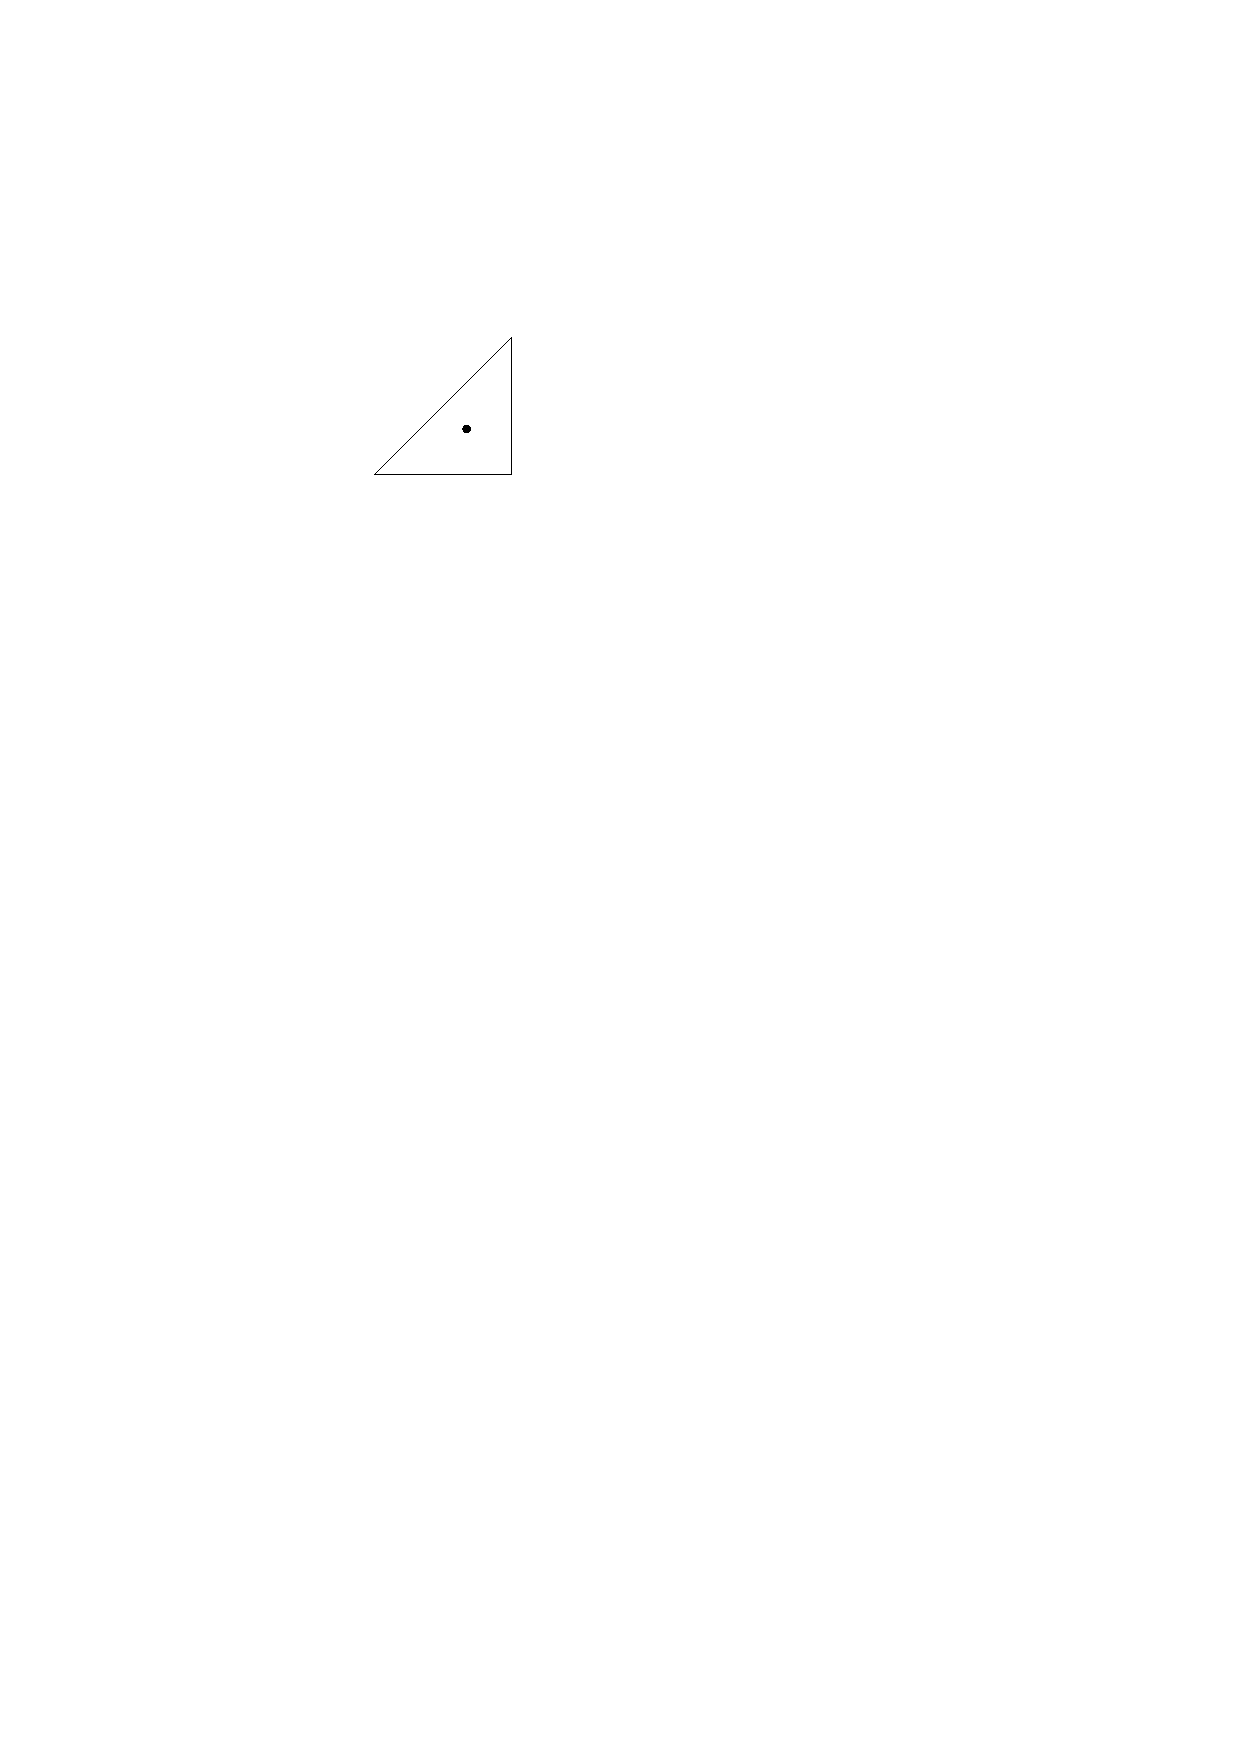
\includegraphics[scale=.8]{figs/killersb-6} \break%
%           $\{\}$ \\
%$\swords$ & 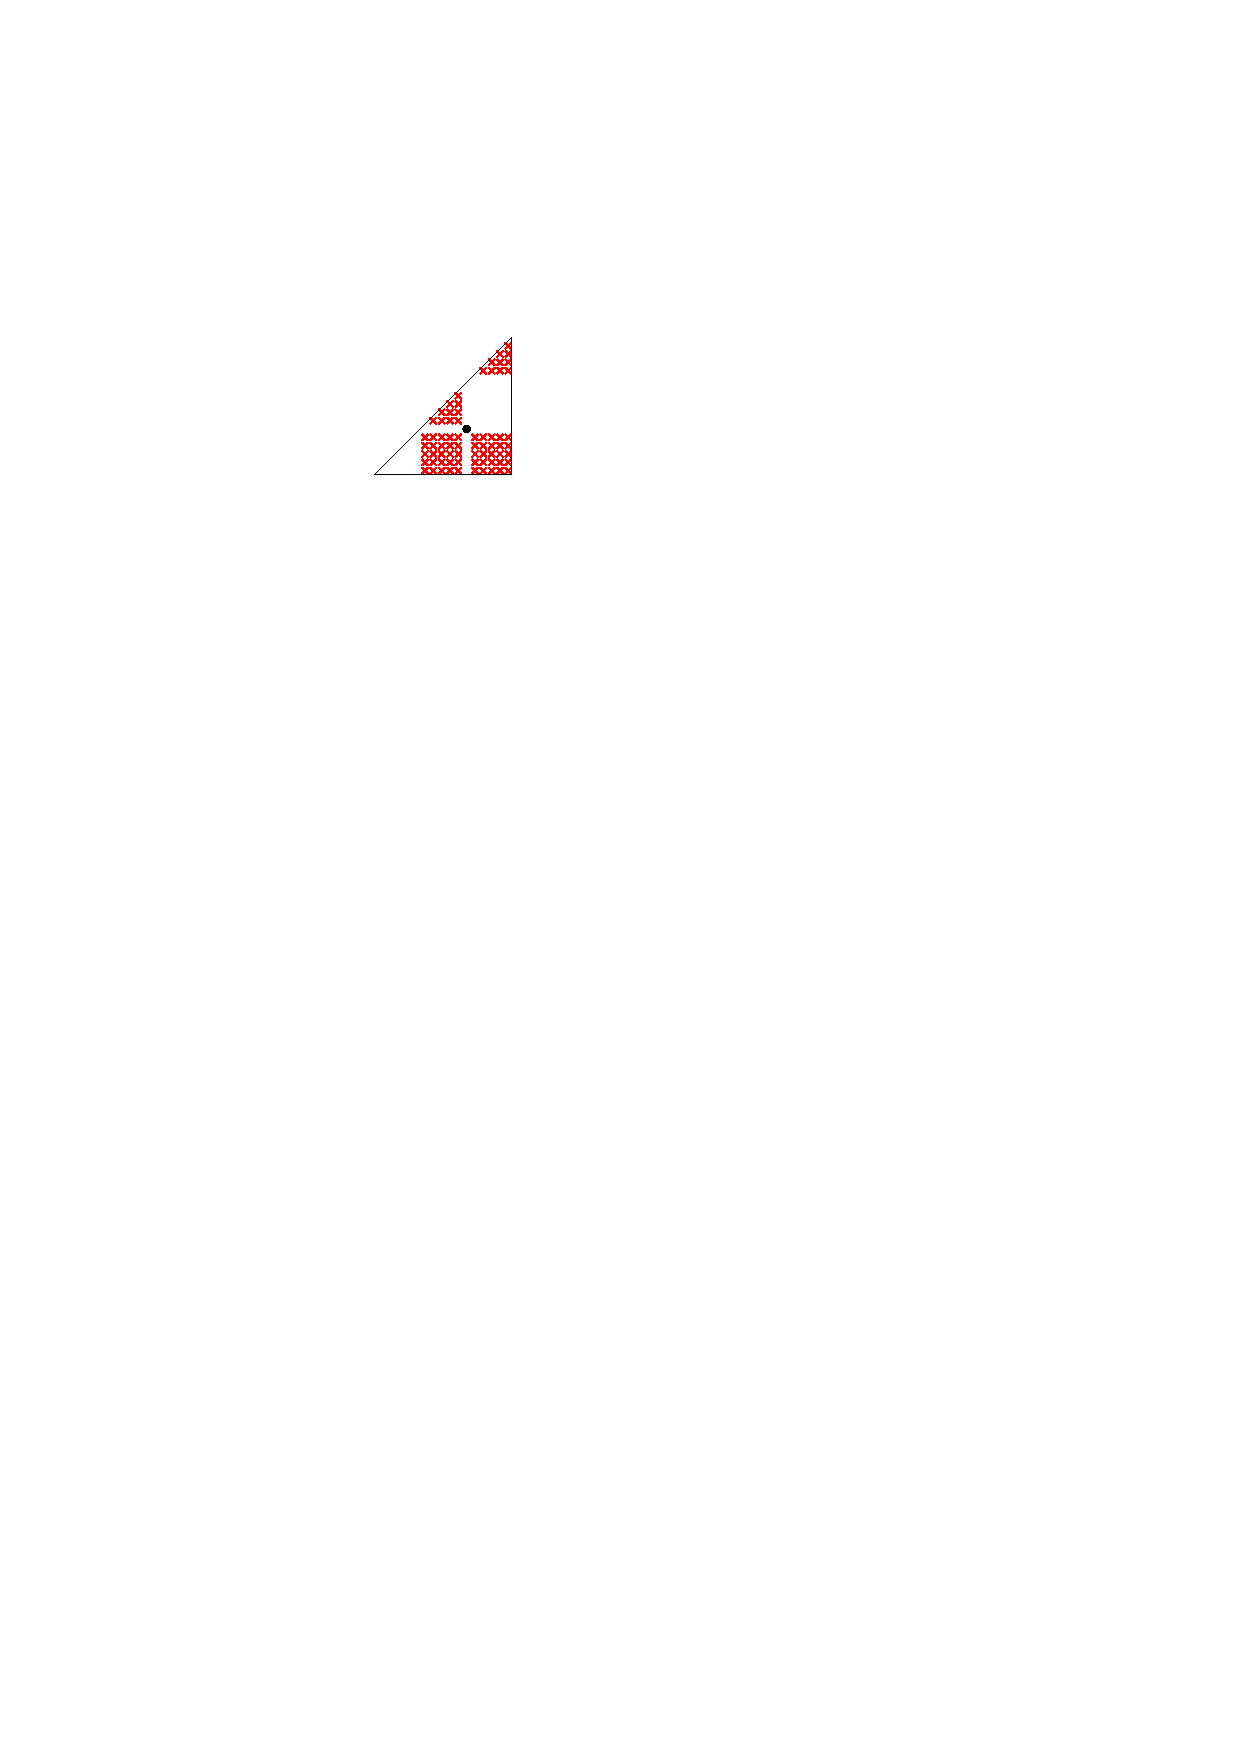
\includegraphics[scale=.8]{figs/killers-7} \break%
%               $\{(x',y'): x'>x, y'< y\}$
%         & 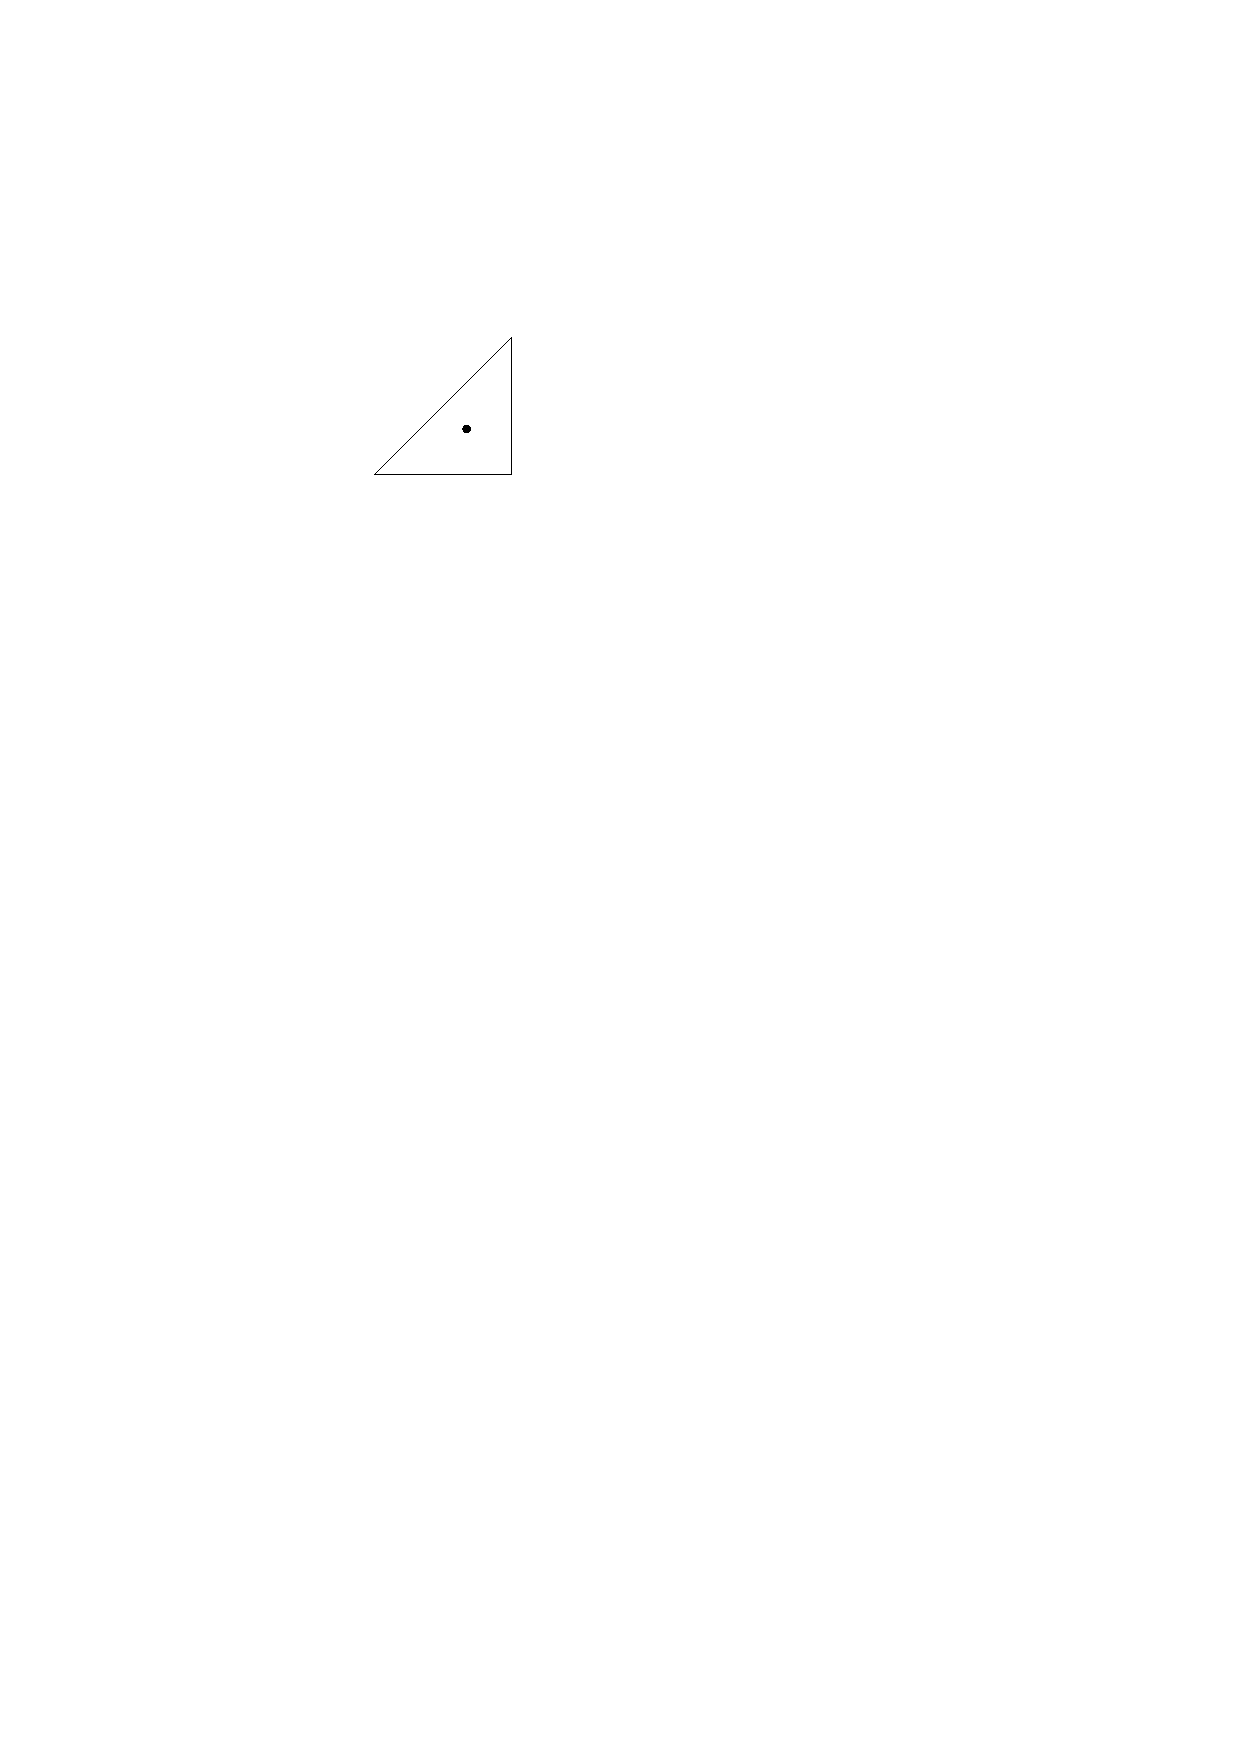
\includegraphics[scale=.8]{figs/killersb-7} \break%
%           $\{\}$ \\
%$\david$ &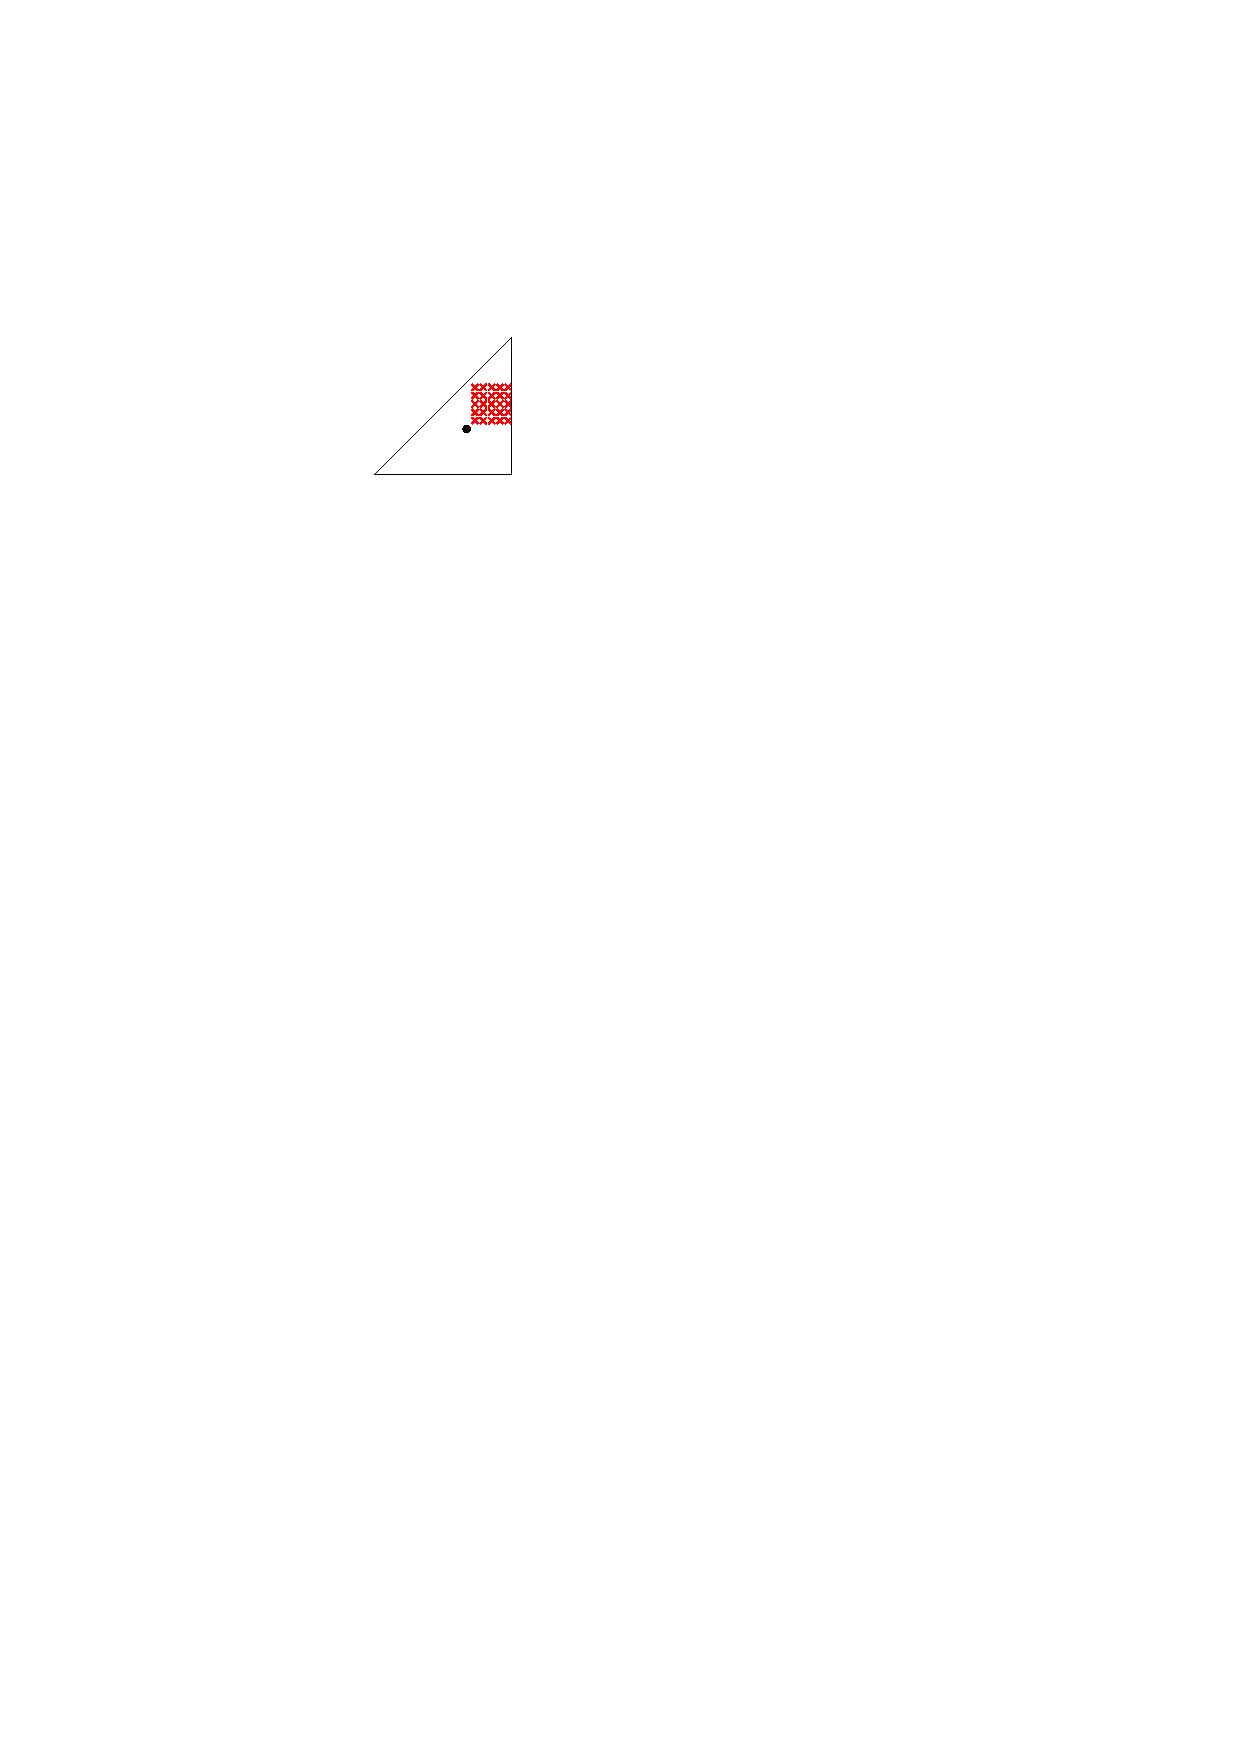
\includegraphics[scale=.8]{figs/killers-8} \break%
%               $\{(x',y'): y < y' <x,\,\, x'>x\}$
%         & 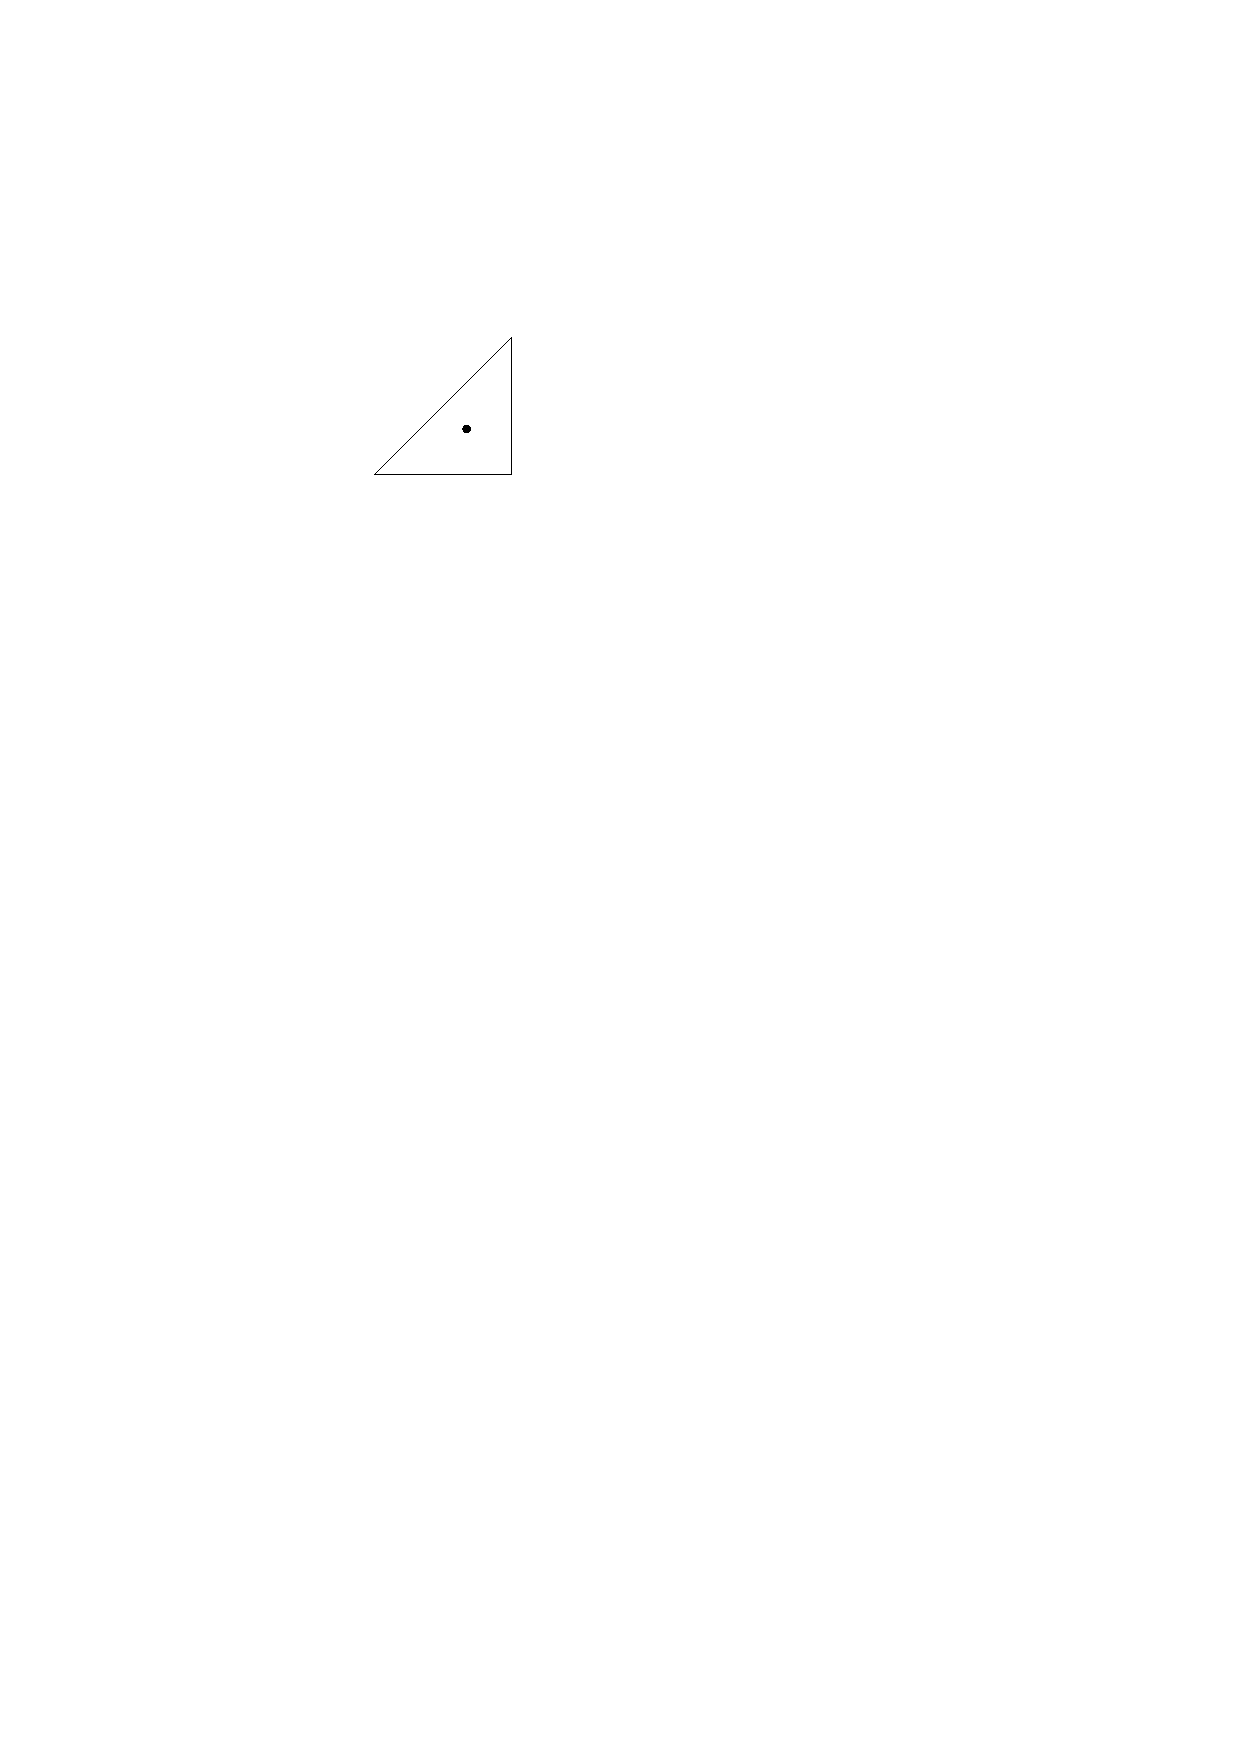
\includegraphics[scale=.8]{figs/killersb-8} \break%
%           $\{\}$ \\
%\end{tabular}
%\end{center}
%   \caption{The restrictions placed on the dot puzzle when for each of 
%     the forbidden subconfigurations.}
%   \tablabel{forbidden}
%\end{table}
%

\begin{figure}
   \begin{center}
      \newlength{\ka}
      \setlength{\ka}{\textwidth}
      \addtolength{\ka}{-1cm}
      \begin{tabular}{c@{\hspace{1cm}}c}
        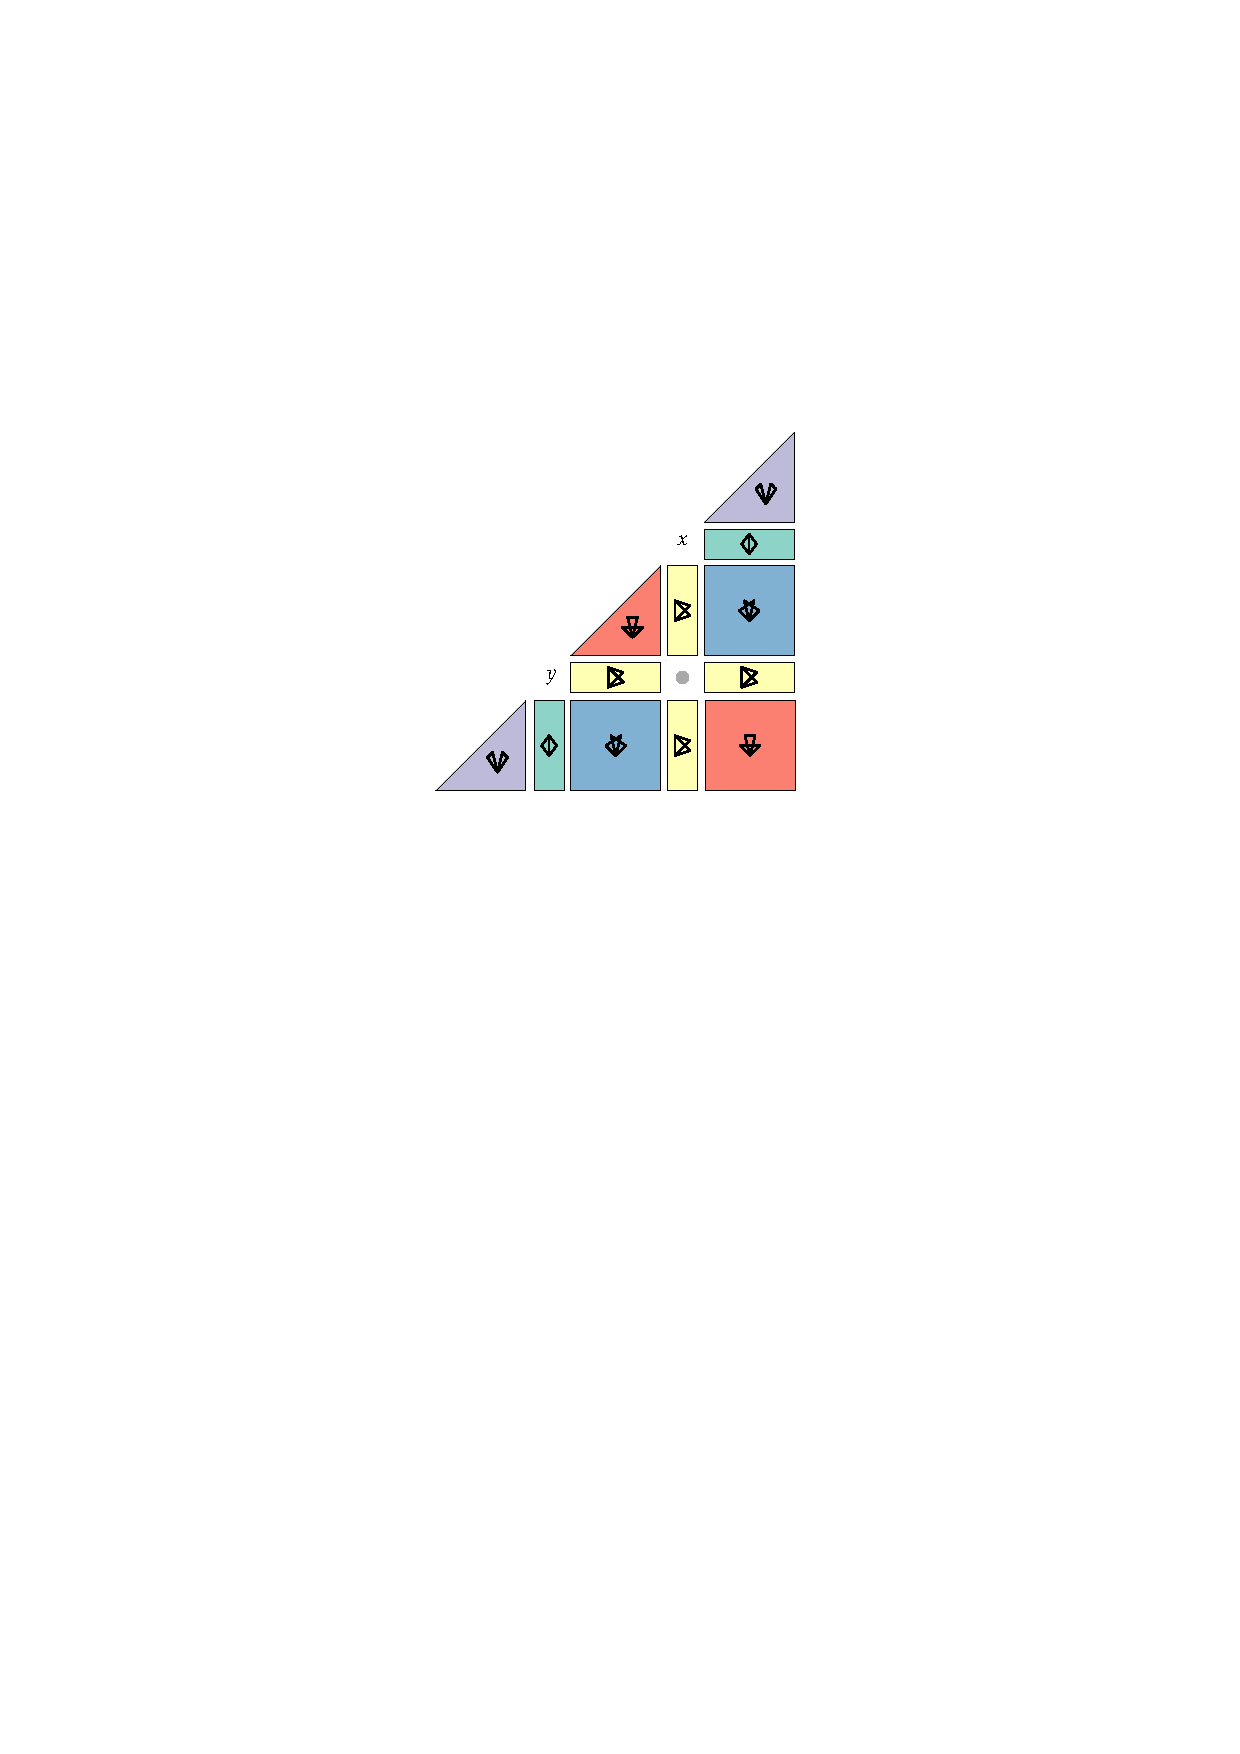
\includegraphics[width=.48\ka]{figs/crapper-2} & 
        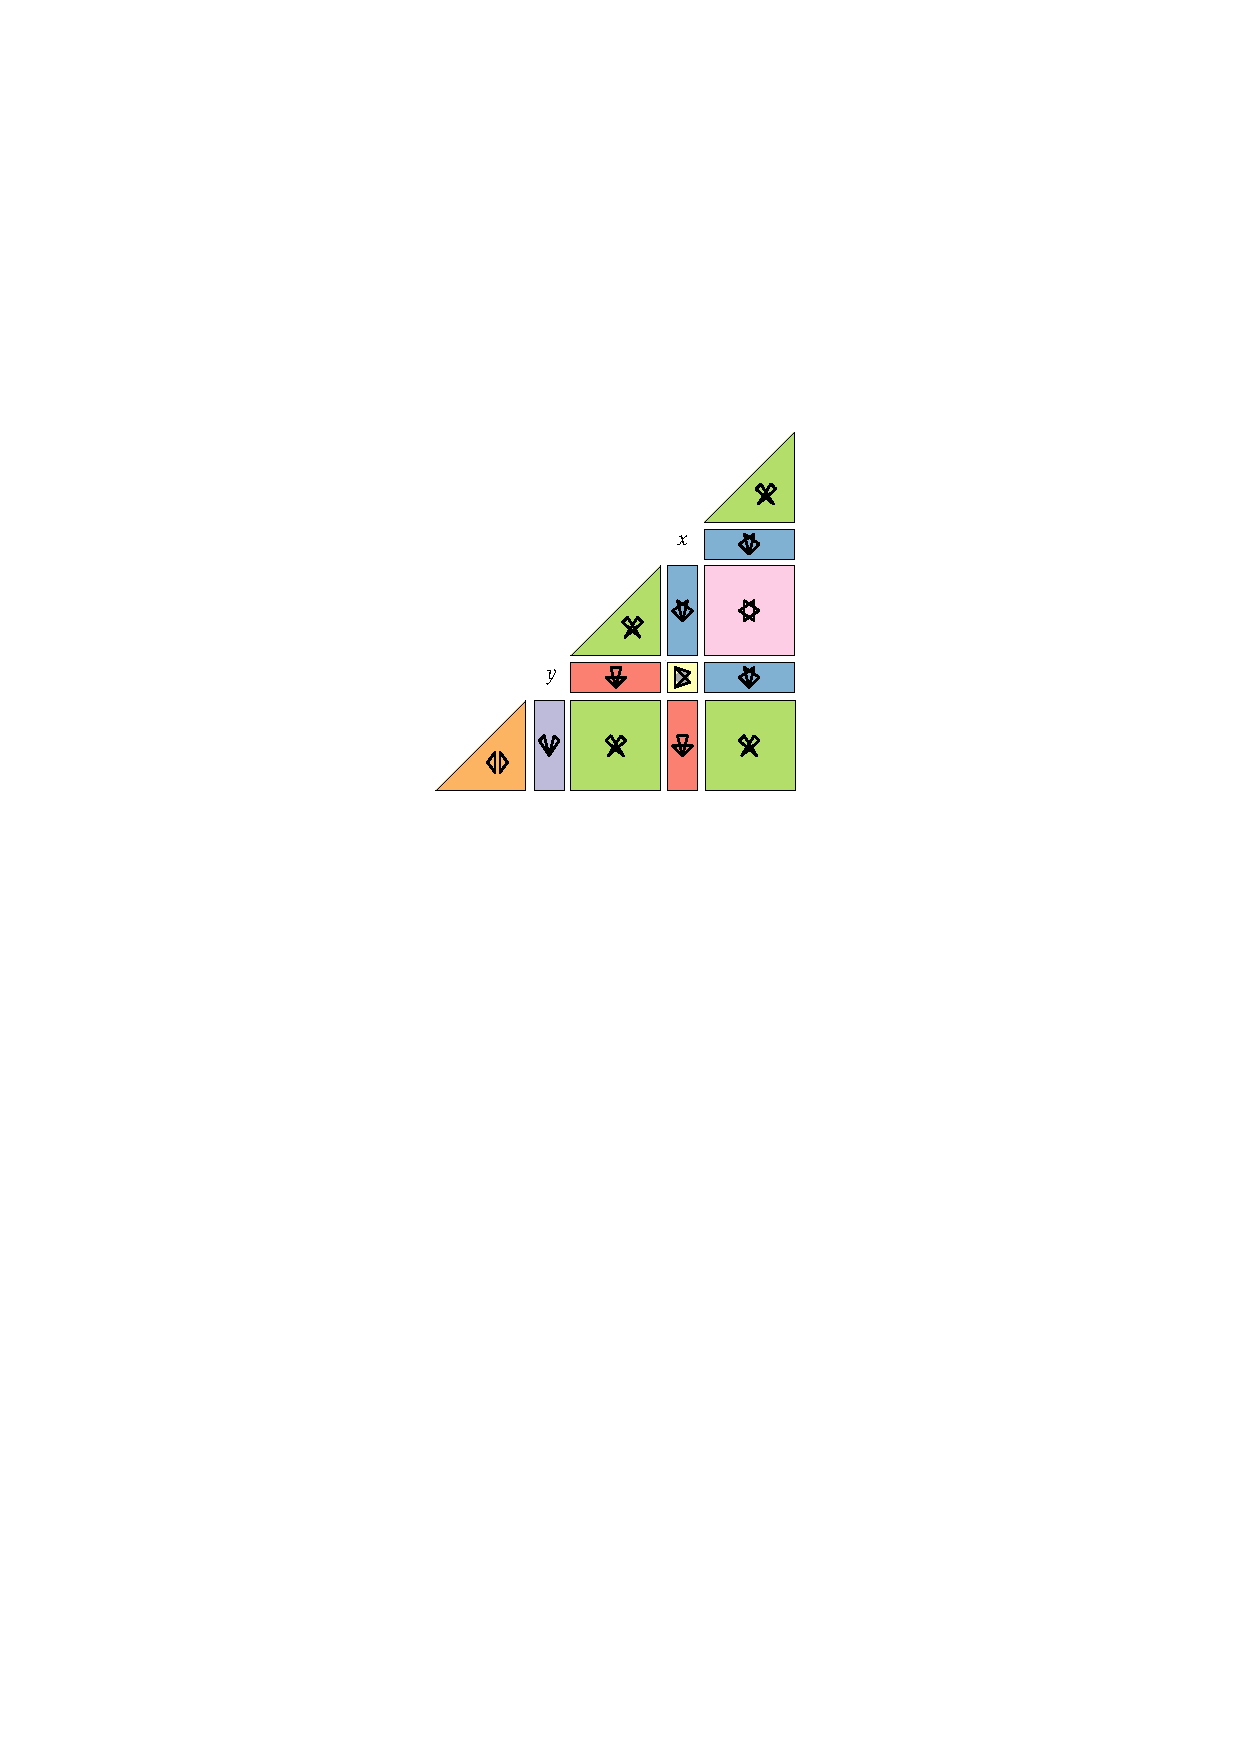
\includegraphics[width=.48\ka]{figs/crapper-1} \\
        (a) & (b)
      \end{tabular}
   \end{center}
   \caption{The regions killed by forbidden configurations during (a)~the current round and (b)~subsequent rounds.}
   \figlabel{forbidden-color}
\end{figure}


\subsection{Some Warm-Up Exercises}

For the remainder of the paper, we will study $\ex'$ using the dot-puzzle
view. Thus, all of our results are bounds on solutions to these dot
puzzles.

We say that a point set is \emph{non-decreasing} (respectively,
non-increasing) if, when sorted lexicographically, the $y$ coordinates of
the points form a non-decreasing (respectively, non-increasing) sequence.
A point set is \emph{increasing} (respectively, decreasing) if it is
non-decreasing (respectively, non-increasing) and it's $x$ coordinates
are distinct.

From \figref{forbidden-color}, some previous upper bounds naturally fall
out.  Consider Bra\ss's results \cite{brass:turan} that $\ex(\nested)\in
O(n^2)$.  For the game defined by $X=\{\nested\}$, we have the rules:
\begin{center}
  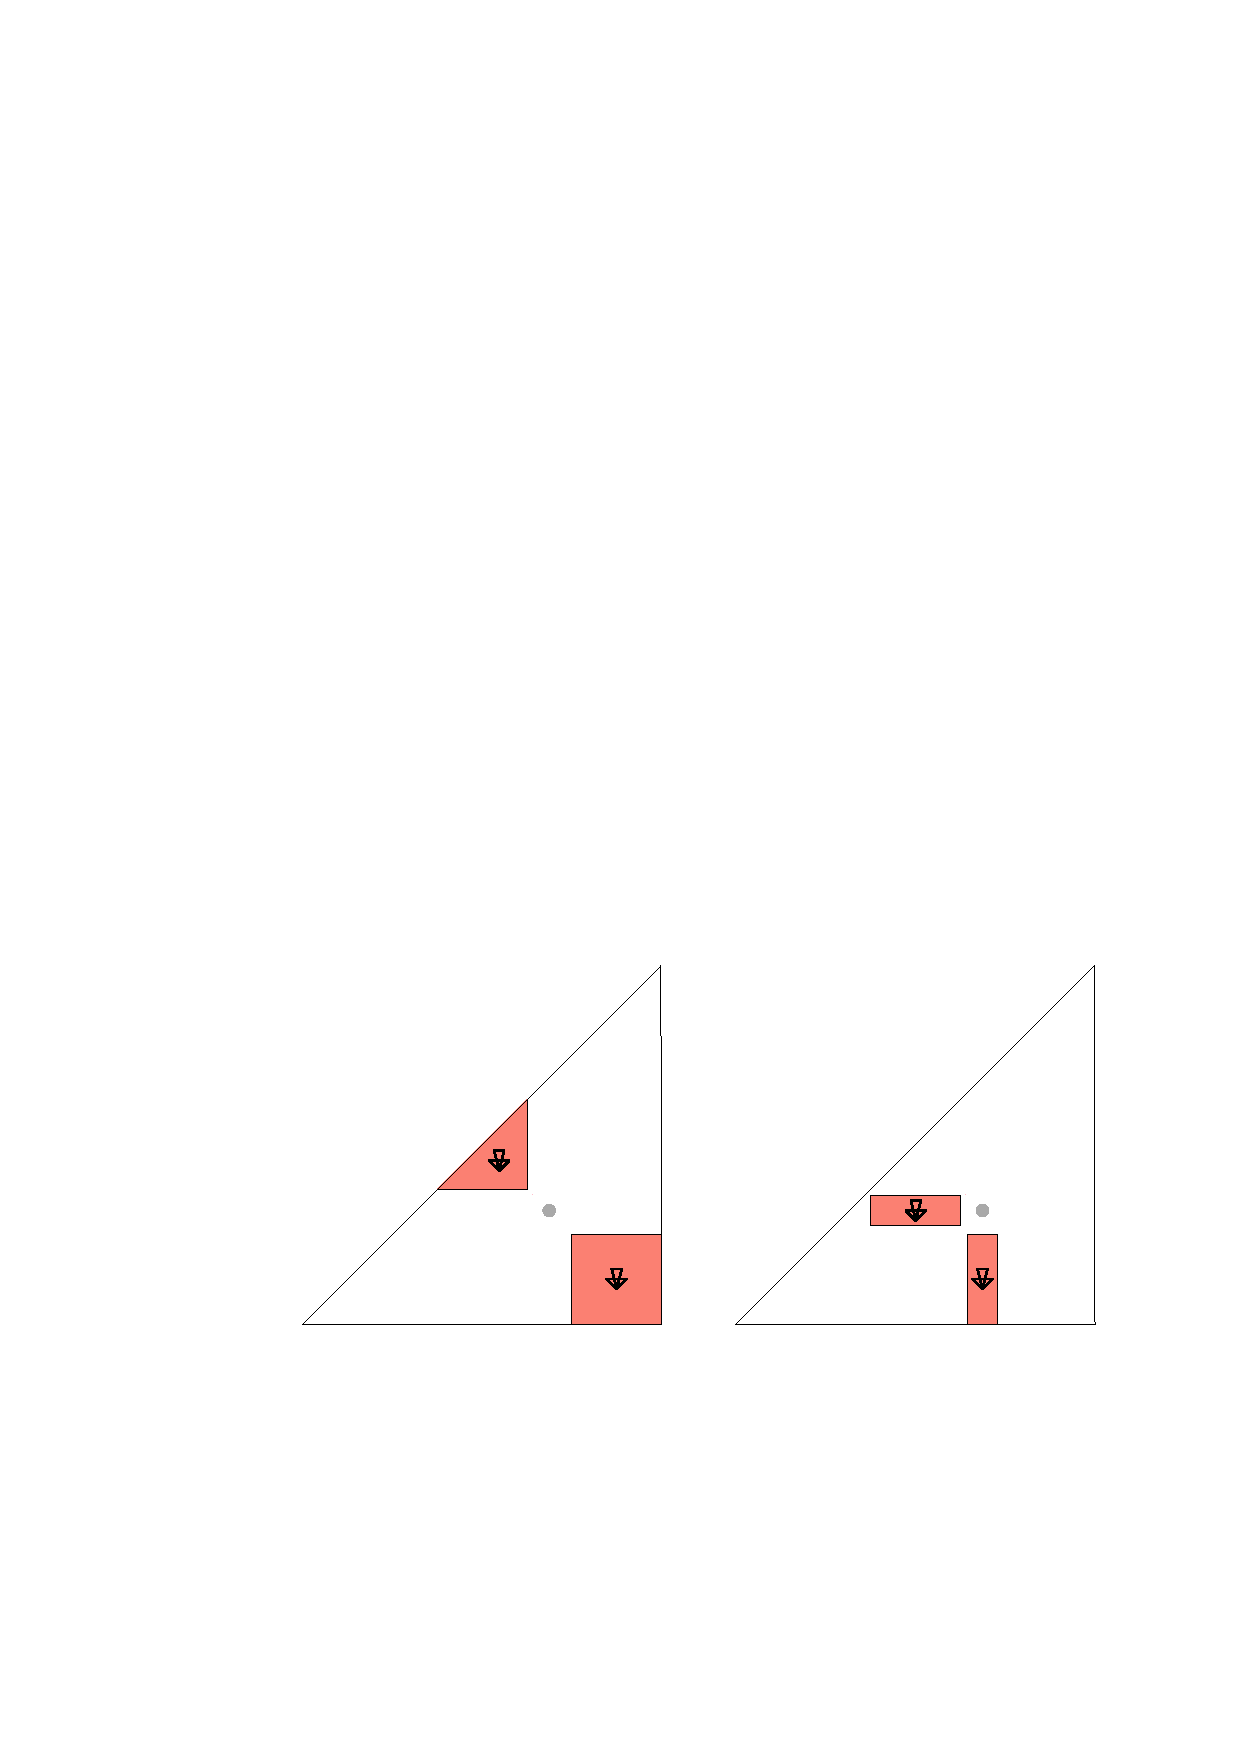
\includegraphics[height=3cm]{figs/helper-3}
\end{center}
In particular, these rules imply that points selected during a
single round of the dot puzzle must be non-decreasing, and thus
at most $2n-3$ points can be selected take part in $Q_i$.  Thus
$\sum_{j=1}^{n}|Q_i| \le 2n^2-3n$, so $\ex'(n,\{\nested\})\in O(n^2)$
and the bound $\ex(n,\{\nested\})\in O(n^2)$ immediately follows from
\lemref{top-bottom}.

Similarly, we can almost recover the result of Bra\ss, Rote and
Swanepoel \cite{brass.rote.ea:triangles} on $\ex(\ears, \swords,
\bat,\nested)$.  Here, the rules are:
\begin{center}
  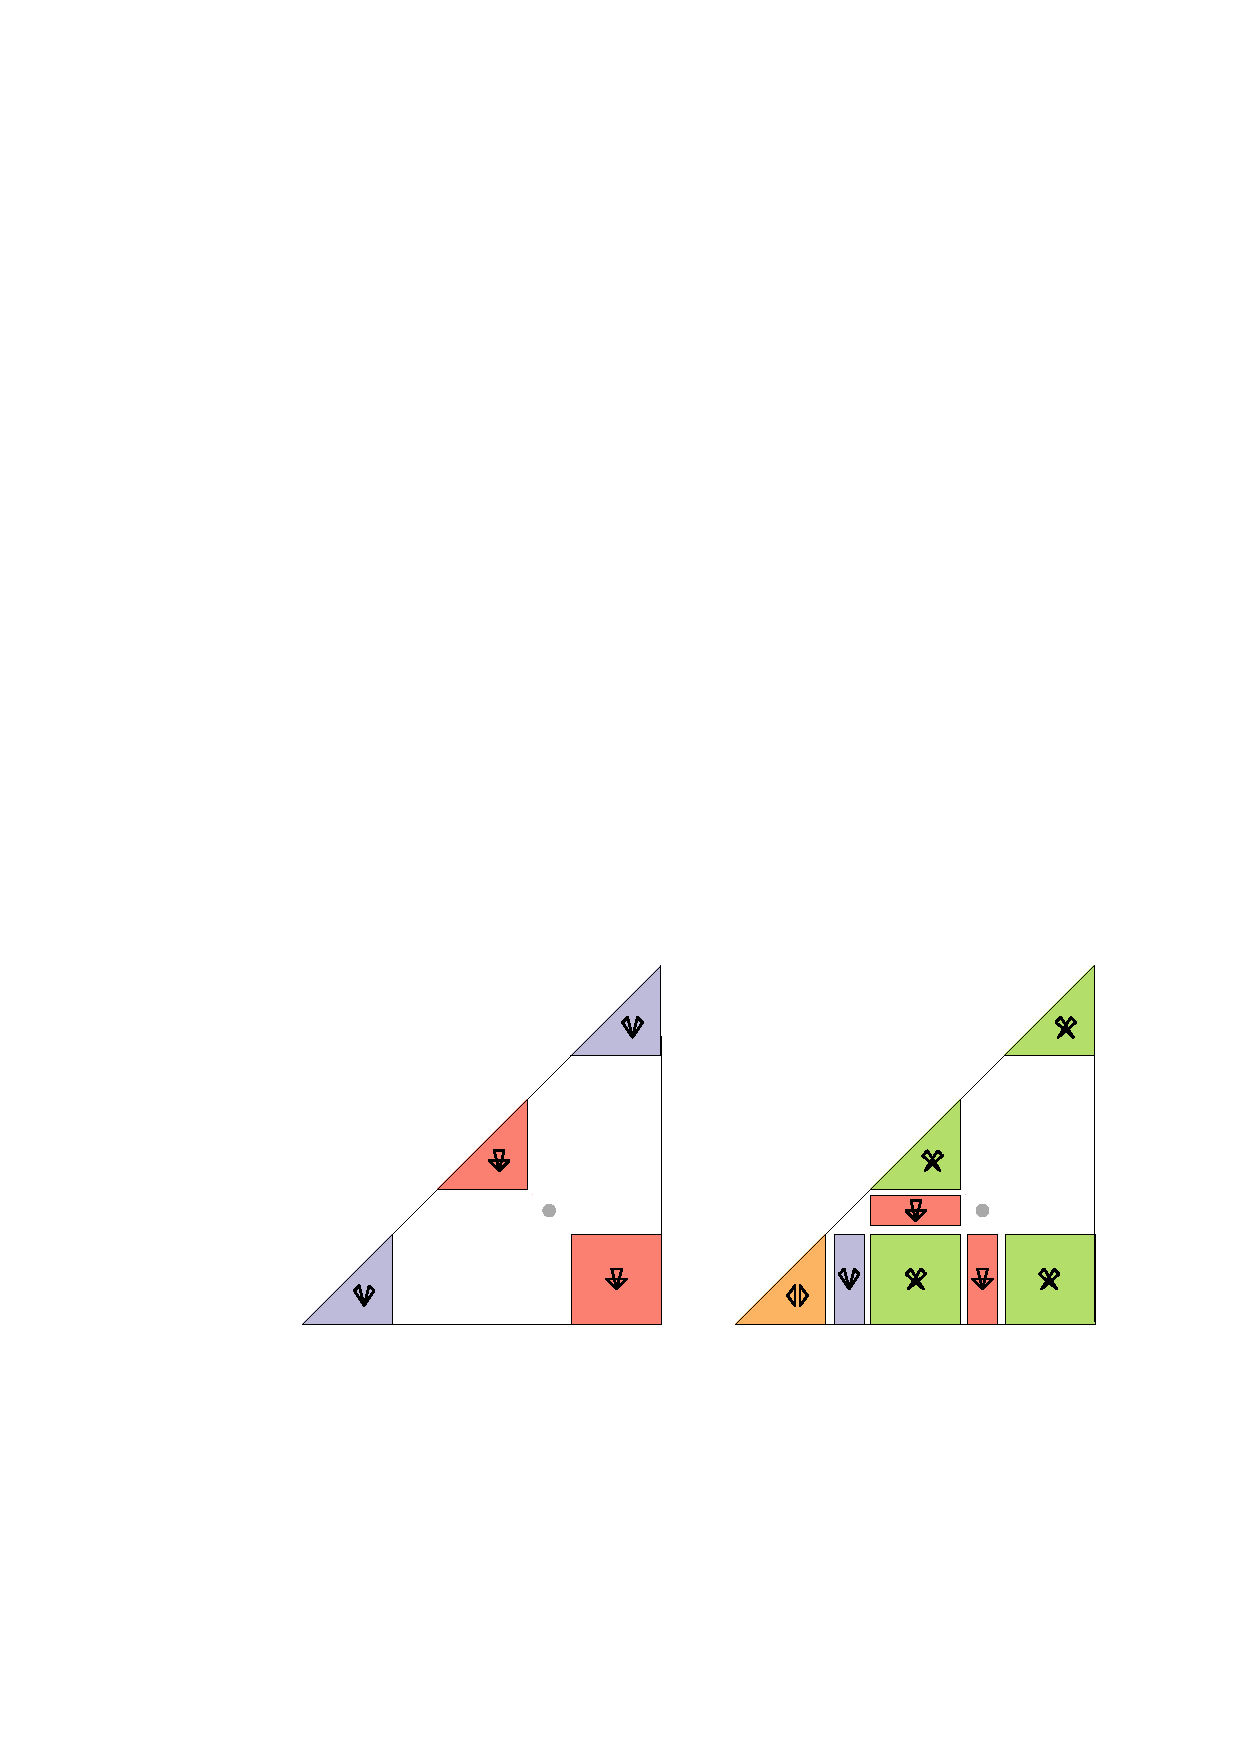
\includegraphics[height=3cm]{figs/helper-2} \enspace ,
\end{center}
The rule for $\nested$
ensures that the set of points taken during a single round form
a non-decreasing point set.  The rules for points allowed in subsequence rounds
ensure
that, after round $i$ any points chosen are either the topmost-rightmost
point in $Q_i$ or are above or to the right of this point.  Taken
together, these rules imply that
\[
    \sum_{i=1}^n|Q_i| \le 3n-4 \enspace ,
\]
since the union of $Q_i$ is a non-decreasing point set (whose size is
therefore at most $2n-3$), and each $Q_i$ shares at most one point with
$Q_{i+1}$.  The bound $\ex(\ears, \swords, \bat,\nested)\in
O(n\log n)$ then follows from \lemref{top-bottom}.


\section{Results Based on Dot Puzzles}
\seclabel{new-results}

% The following is the start of some bullshit argument, unless I can fix it.

%Earlier, we showed that the inclusion of the $\mariposa$ configuration in
%the set of excluded configurations, $X$, has no effect on the asymptotics
%of $\ex(n,X)$.  Here we show that a similar, though slightly weaker,
%result for the $\nested$ configuration.
%
%\begin{lem}
%  $\ex'(n,\{\taco,\bat\}\cup X) \in \Omega(\ex'(n,\{\taco\}\cup X)/\log n)$.
%\end{lem} 
%
%\begin{proof}[Proof Sketch]
%    Assume without loss of generality that $n$ is a power of 2 Partition
%    $Q$ into $O(\log n)$ \emph{layers}, where layer 0 contains
%    the \emph{square}, $L_0=\{(x,y)\in Q: x\ge n/2,\, y\le n/2\}$.
%    Subsequent layers are obtained by recursing on the two triangles in
%    $Q\setminus L_0$, so that $L_1$ contains two squares, $L_2$ contains
%    four squares, and so on.
%
%    Let $Q_1,\ldots,Q_n$ be a play of the dot-puzzle that achieves
%    $\ex'(n,\{\taco\}\cup X)$ while avoiding $\{\taco\}\cup X$
%    configurations.  Observe that, because we exclude $\taco$, the sets
%    $Q_i$ and $Q_j$ are disjoint for all $1\le i<j\le n$.
%
%    Then, for any layer $L_i$, the sets $Q_1\cap L_i,\ldots,Q_n\cap L_i$
%    avoid all configurations in $\{\taco\}\cup X$ as well as $\bat$
%    configurations.  By the pigeonhole principle, one of these layers,
%    say $L_i$, has size $\Omega(\ex'(n,\{\taco\}\cup X)/\log n)$.
%
%
%
%points that maximize
%\end{proof}
%
%is irrelevan
%

After this warm-up, and with the dot-puzzle view, we are ready to prove
some new results.  We begin with a collection of results on forbidding
the $\swords$ configuration.

\subsection{Forbidding Crossing Vertex-Disjoint Triangles}

In this section, we focus on the configuration $\swords$ and give
linear upper bounds bounds on $\ex'(n,\{\swords, Y\})$ for each
$Y\in\{\taco,\nested,\crossing\}$.  In \secref{lower-bounds}, we show
that $\ex'(n,\{\swords,\mariposa,\bat,\ears,\david\})\in \Omega(n^2)$.
Together, these two results completely determine $\ex'(n,\{\swords\}\cup
X\})$ for any $X$.

In the following, we use the notation $\xmin(S)$ to denote the
minimum $x$-coordinate of any point in the point set $S$.  
%If $S$ is empty, then we define $\xmin(S)$ as $n+1$.  
We define $\ymin(S)$,
$\xmax(S)$, and $\ymax(S)$ similarly.
%, except that $\ymin(\emptyset) = n$, $\ymax(\emptyset)=0$, and 
% $\xmax(\emptyset)=1$.  
For any
$X\subset\{\taco,\mariposa,\bat,\nested,\crossing,\ears,\swords,\david\}$
and any $S\subset Q$, we define $\survivors(X,S)$ to be the subset of
points in $Q$ that can still be played in the dot-puzzle game if the
points is $S$ have been played in previous rounds.

%FIXME: The following observation is totally incorrect.  A sequence of points close to the boundary can generate a whole bunch of uncovered rectangles:
%
%\begin{center}
%   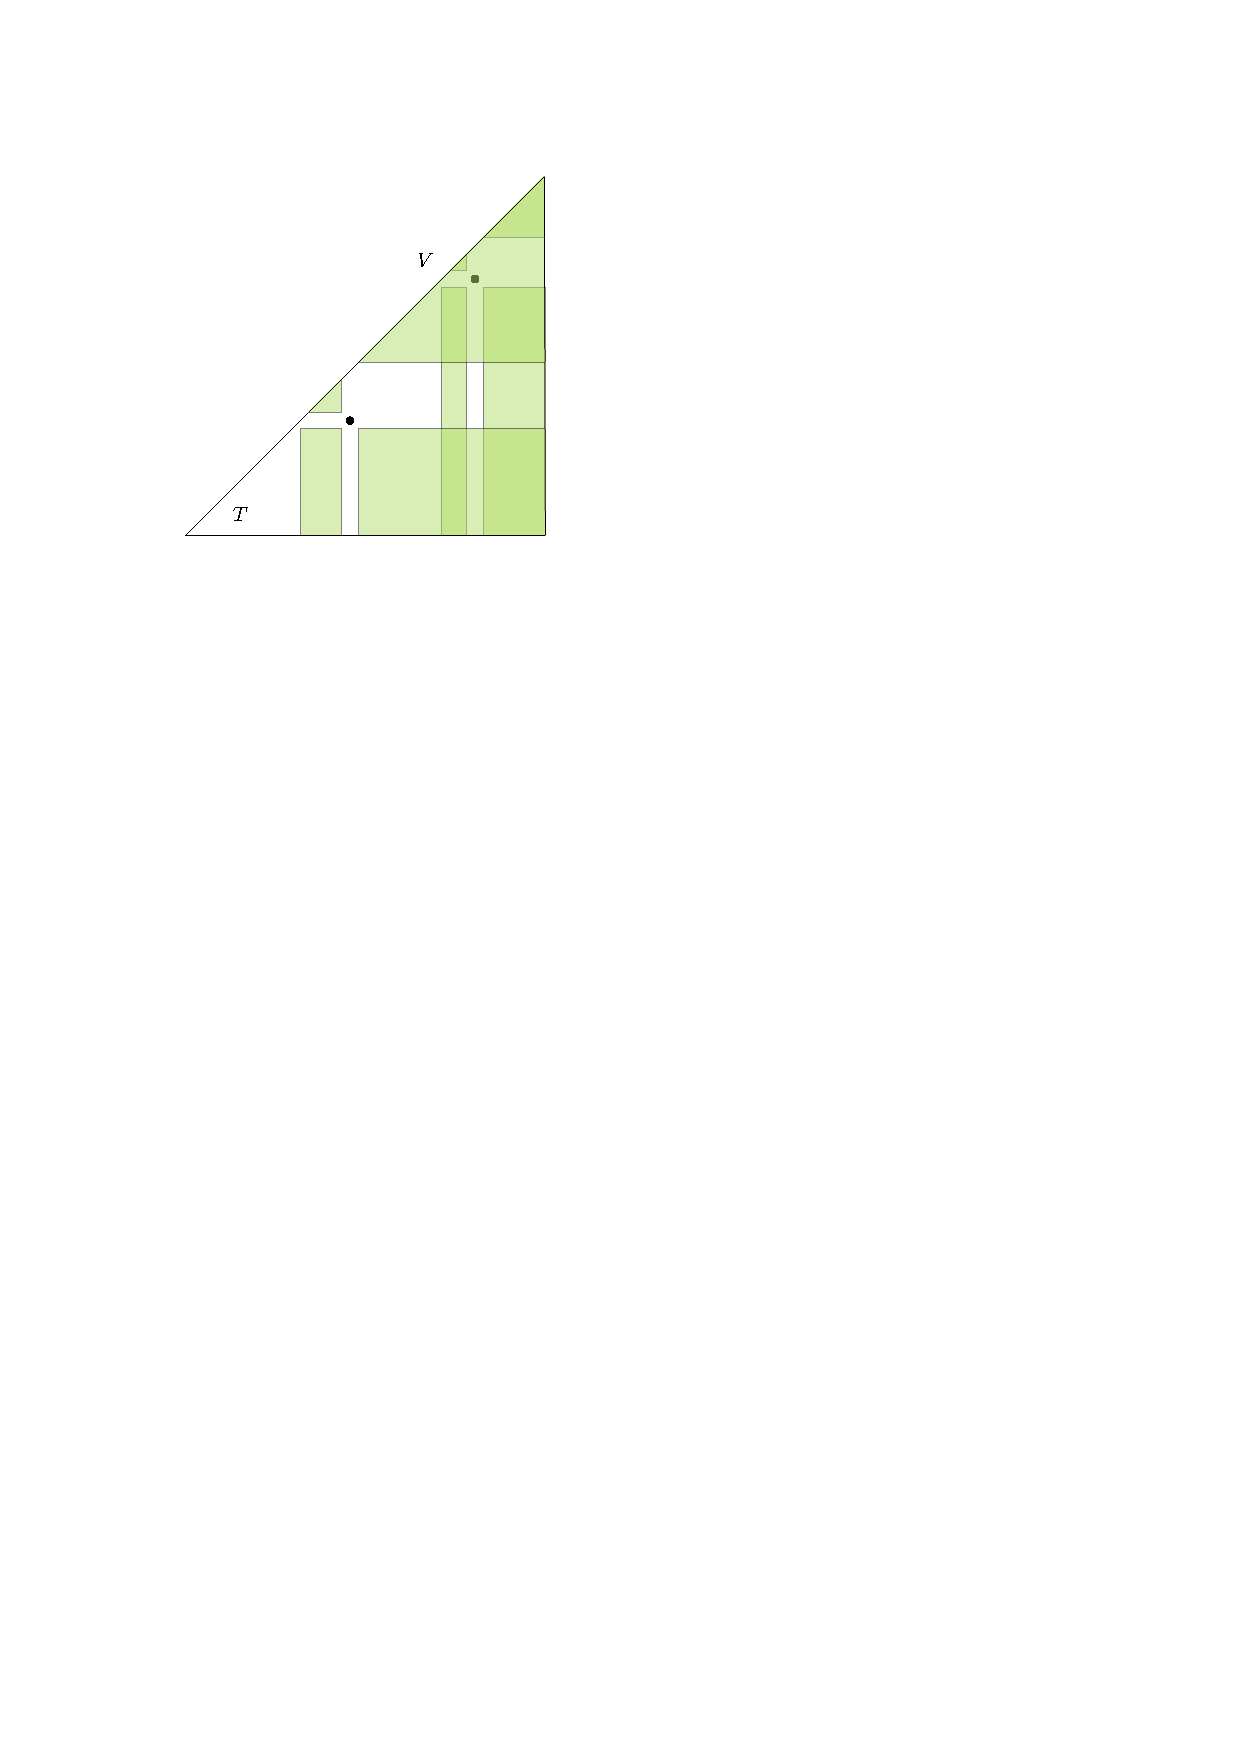
\includegraphics{figs/survivors-ce}
%\end{center}
%
% The fix was implemented by defining the ymax coordinate in terms of $S^*$.

\begin{obs}\obslabel{swords-region}
  (Refer to \figref{survivors}.)  Let $S$ be any non-empty
  subset of $Q$ and let $S^{*}= \{(x,y)\in S : y \le \xmin(S)\}$.
  Then $\survivors(\{\swords\},S)$ is contained in the union of
  a \emph{triangular region} $T=\{(x,y)\in Q: x\le \ymin(S)+1\}$,
  a \emph{rectangular region} $R=\{(x,y)\in Q: x\ge \xmax(S^*),\,
  \ymax(S^*) \le y\le \xmin(S)\}$, a \emph{vertical line} $V$ passing
  through the rightmost point of $S$ with maximum $y$-coordinate, a
  \emph{horizontal line} $H^{\min}=\{(x,y)\in Q: y=\ymin(S)\}$ and a
  horizontal line $H^{\max}=\{(x,y)\in Q: y=\ymax(S^*)\}$.
\end{obs}

\begin{figure}
  \begin{center}
    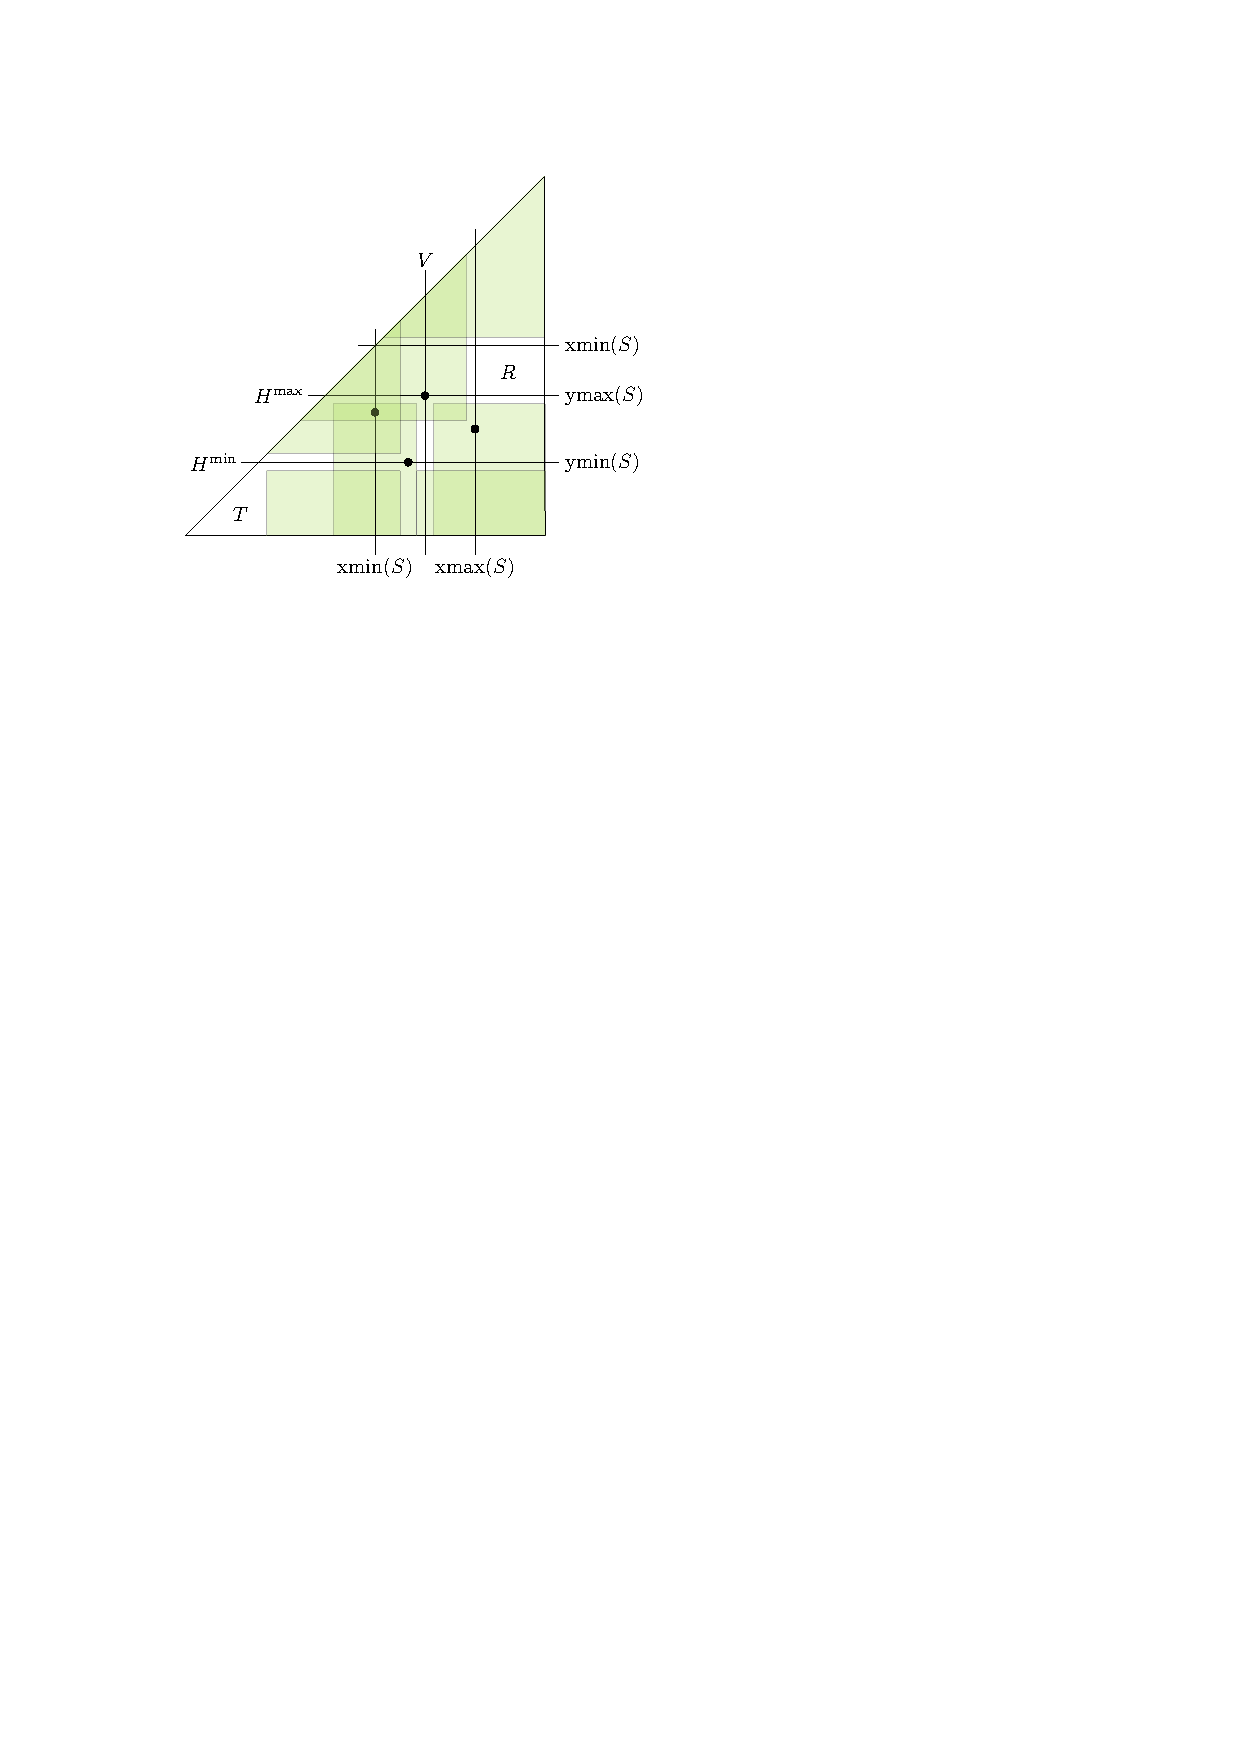
\includegraphics{figs/survivors}
  \end{center}
  \caption{An illustration of \obsref{swords-region}.}
  \figlabel{survivors}
\end{figure}

\begin{proof}
  The points defining $\ymax(S^*)$ and $\xmin(S)$ cover everything
  below $H^{\max}$, except $H^{\min}$, $V$, and $T$.  Above $H^{\max}$,
  the point defining $\xmax(S^*)$ covers everything to the left of $R$
  and the point defining $\xmin(S)$ covers everything above $R$.  Thus,
  everything except $T$, $R$, $V$, $H^{\min}$ and $H^{\max}$ is covered.
\end{proof}

\obsref{swords-region} gives us a form of \emph{potential function} that
we can use.  We will apply it with $S=\bigcup_{j=1}^i Q_j$ so that as
rounds proceed, any time the value of $\xmax(S)$ or $\ymax(S)$ increases,
the size of the rectangle $R$ decreases. Any time the value of $\ymin(S)$
decreases, the size of the triangle $T$ decreases.  So that we can refer
to these point sets as they change, we let $S_i=\bigcup_{j=1}^i Q_i$
$S_i^{*} = \{(x,y)\in S_i : y\le \xmin(S_i)\}$, and we define $T_i$,
$R_i$, $V_i$, $H^{\max}_i$, and $H^{\min}_i$ as in \obsref{swords-region},
but with respect to the set $S=S_i$. So that $V_i$ is unambiguous, we
define it as the vertical line passing through the rightmost point in
$S_i$ whose $y$-coordinate is equal to $\ymax(S_i)$.

\begin{thm}\thmlabel{taco-swords}
  $\ex'(n,\{\taco,\swords\}) \in O(n)$.
\end{thm}

\begin{center}
   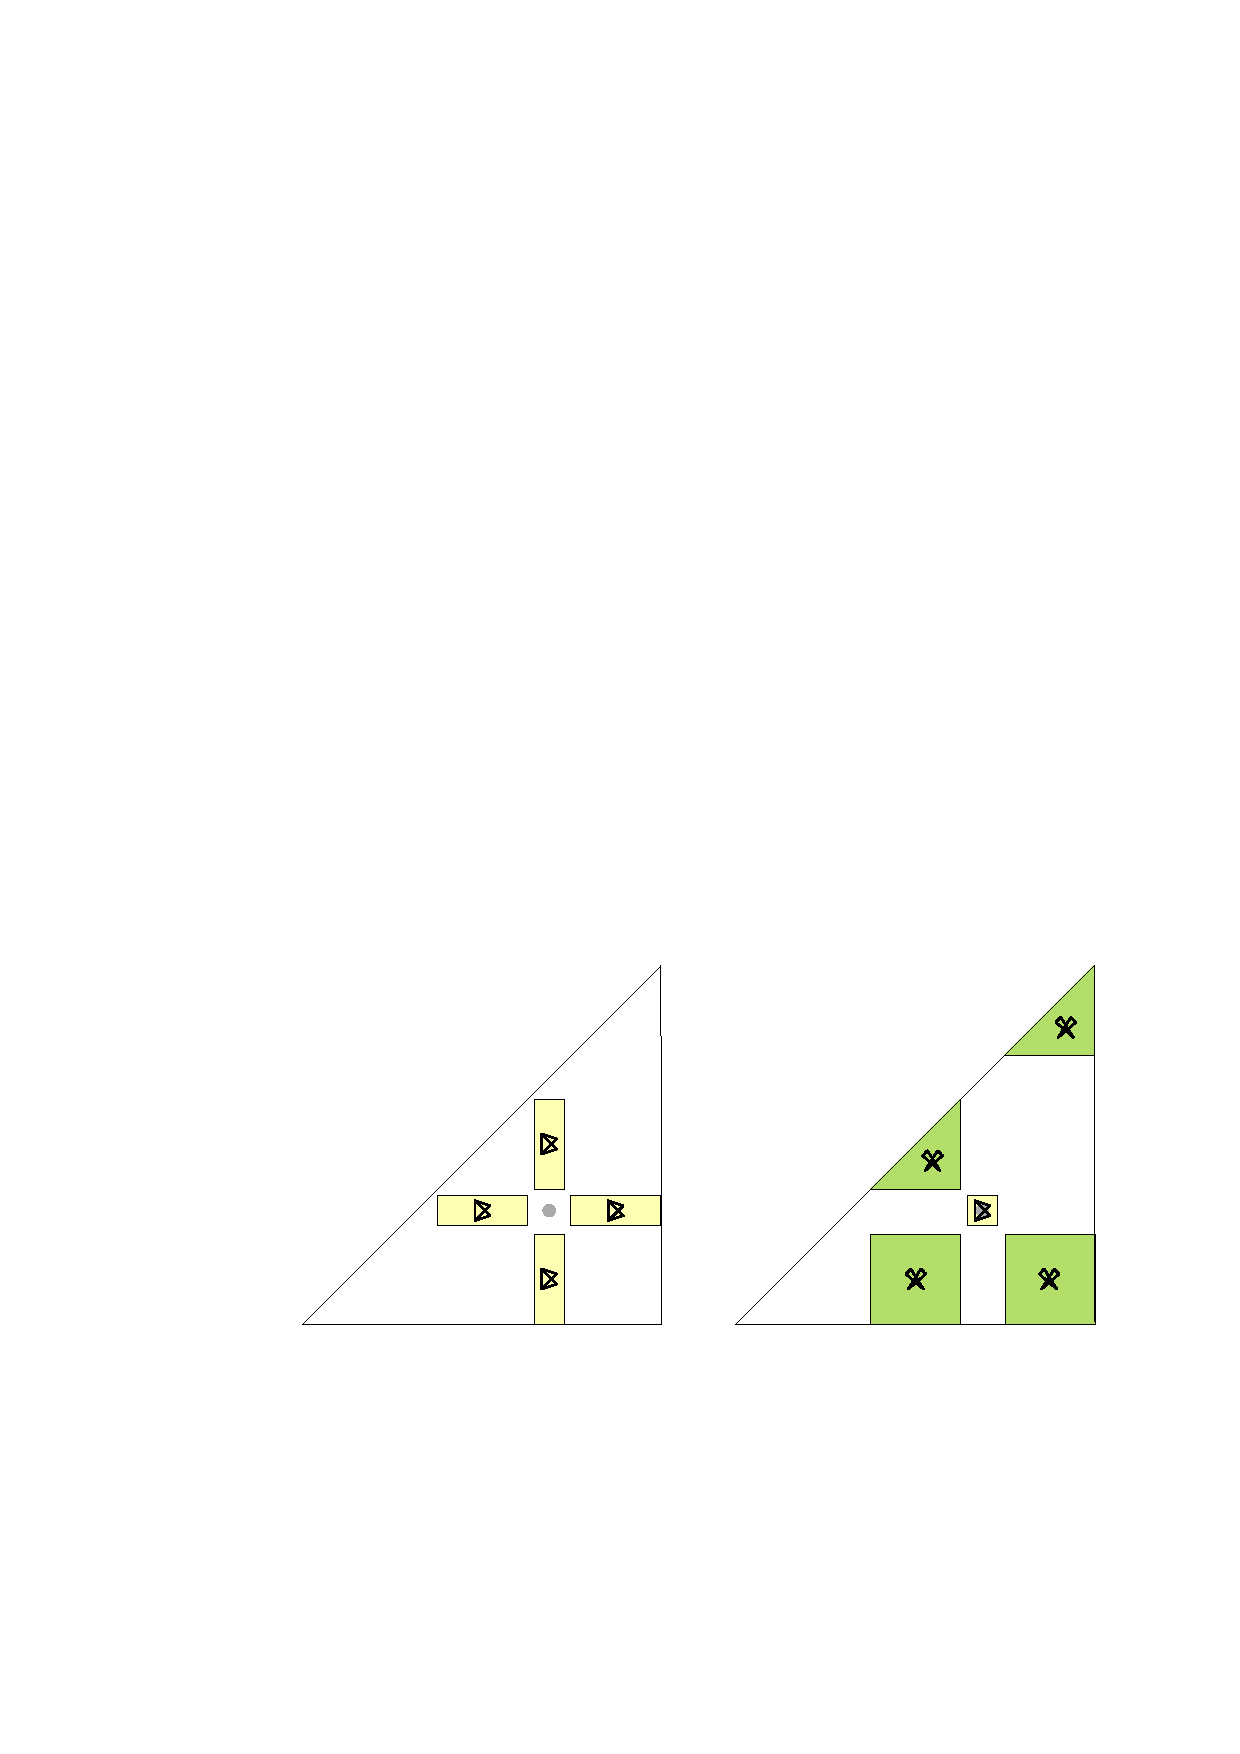
\includegraphics[height=3cm]{figs/helper-6}
\end{center}

\begin{proof}
  We will directly bound $\sum_{i=1}^n |Q_i|$.  We begin by noting that,
  since we forbid $\taco$, the set of points in each $Q_i$ contains
  at most one point from each row and each column.  We will use this
  fact implicitly for the rest of the proof.

  Now, observe that if $Q_i$ contains $t_i\ge 2$ points in $T_i$, then
  $\ymin(S_{i+1}) \le \xmin(S_i)-t_i+2\}$.  This immediately
  implies that $\sum_{i=1}^n t_i \le 3n$.

  Similarly, if $Q_i$ contains $r_i\ge 1$ points in $R_i$, then
  $\ymax(S_{i+1}^*)\ge \ymax(S_i^*)+r_i-1$.  This immediately
  implies that $\sum_{i=1}^n r_i\le 2n$.
  
  Finally, we observe that $Q_i$ contains at most one point each from
  $H^{\min}_i$, $H^{\max}_i$, and $V_i$, so
  \[
      \sum_{i=1}^{n}|Q_i| \le \sum_{i=1}^n(t_i+r_i+3) \le 8n \enspace . \qedhere
  \]
\end{proof}

Our next two results have similar proofs to that of \thmref{taco-swords},
but they require a little more care to bound the number of points that
appear in the horizontal lines $H^{\max}_i$, $H^{\min}_i$ and $V_i$.

\begin{lem}
  Let $Q_1,\ldots,Q_n$ be a solution to a dot-puzzle game that includes
  the rules for $\swords$.  Then, $V_{i+1}$
  \begin{enumerate}
    \item $\xmin(S_{i+1}) \le \xmin(S_i)$;
    \item $\ymax(S_{i+1}^*) \le \ymin(S_ii^*)$;
    \item $\ymax(S_{i+1}^*) \le \ymin(S_ii^*)$;

 
  \[ \sum_{i=1}^{n}\left(|Q_i\cap V_i|+|Q_i\cap H^{\max}_i|+|Q_i\cap H^{\min}_i|\right) \in O(n) \enspace . \]
\end{lem}

\begin{thm}\thmlabel{nested-swords}
  $\ex'(n,\{\nested,\swords\}) \in O(n)$.
\end{thm}

\begin{center}
   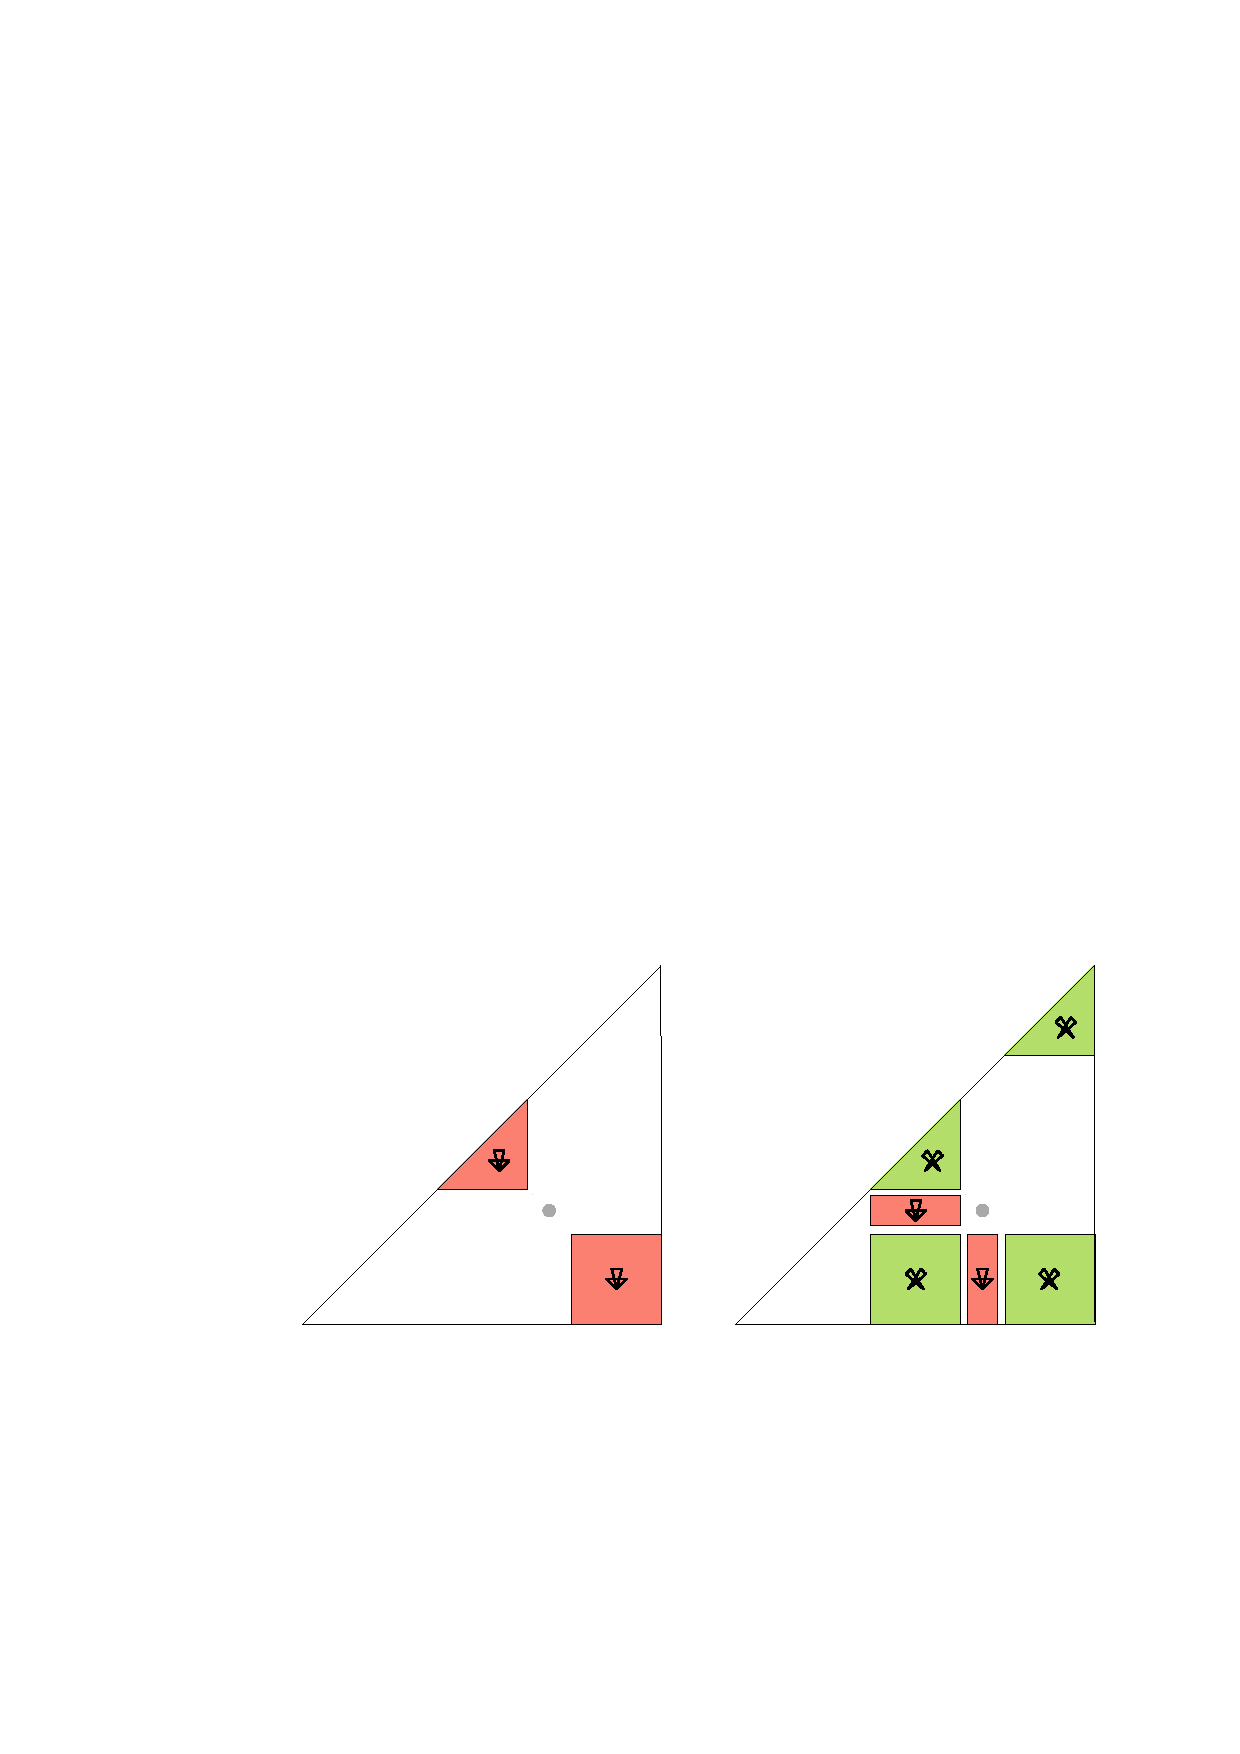
\includegraphics[height=3cm]{figs/helper-7}
\end{center}

\begin{proof}
   The proof is similar to the proof of \thmref{taco-swords}.
   The forbidden configuration $\nested$ implies that each set $Q_i$
   must be non-decreasing (see \figref{forbidden-color}a).
   We will use this fact implicitly for the rest of the proof.

   Now, if $Q_i$ contains $t_i$ points in $T_i$, then the fact
   that $Q_i$ is non-decreasing implies that $\ymin(S_{i+1})\le
   \ymin(S_i)-\lfloor t_i/2 \rfloor$.  This immediately implies that
   $\sum_{i=1}^n t_i \le 3n$.

   Similarly, if $Q_i$ contains $r_i\ge 1$ points in $R_i$, then the fact
   that $Q_i$ is non-decreasing means that
   \[
       \ymax(S_{i+1})+\xmax(S_{i+1}) 
             \ge \ymax(S_{i})+\xmax(S_{i}) + r_i - 1 \enspace .
   \]
   This immediately implies that $\sum_{i=1}^n r_i \le 3n$.

   To account for points of $Q_i$ on the vertical line $V_i$, we consider
   the lowest point of $\survivors(\{\swords\},Q_i)$ on  
   $V_i\setminus T_i\setminus R_i$ and denote the $y$-coordinate of this
   point by $y_i$.  If $V_i\setminus T_i\setminus R_i$ contains $v_i\ge
   1$ points of $Q_i$, then $y_{i+1}\ge y_i+v_i-1$.  This immediately
   implies that $\sum_{j=1}^n v_i \le 2n$.

   Accounting for points of $Q_i$ on the horizontal lines $H^{\min}_i$ and $H^{\max}_i$ is similar,
   but with respect to the left-most point of 
   $\survivors(\{\swords\},Q_i)$ in $H^{\min}_i\setminus T_i\setminus R_i$
   and $H^{\max}_i\setminus T_i\setminus R_i$.

   Summing everything, we find that
   $\ex'(n,\{\swords,\nested\})\le\sum_{j=1}^n |Q_i|\le 12n$.
\end{proof}


\begin{thm}\thmlabel{crossing-swords}
  $\ex'(n,\{\crossing,\swords\}) \in O(n)$.
\end{thm}

\begin{center}
   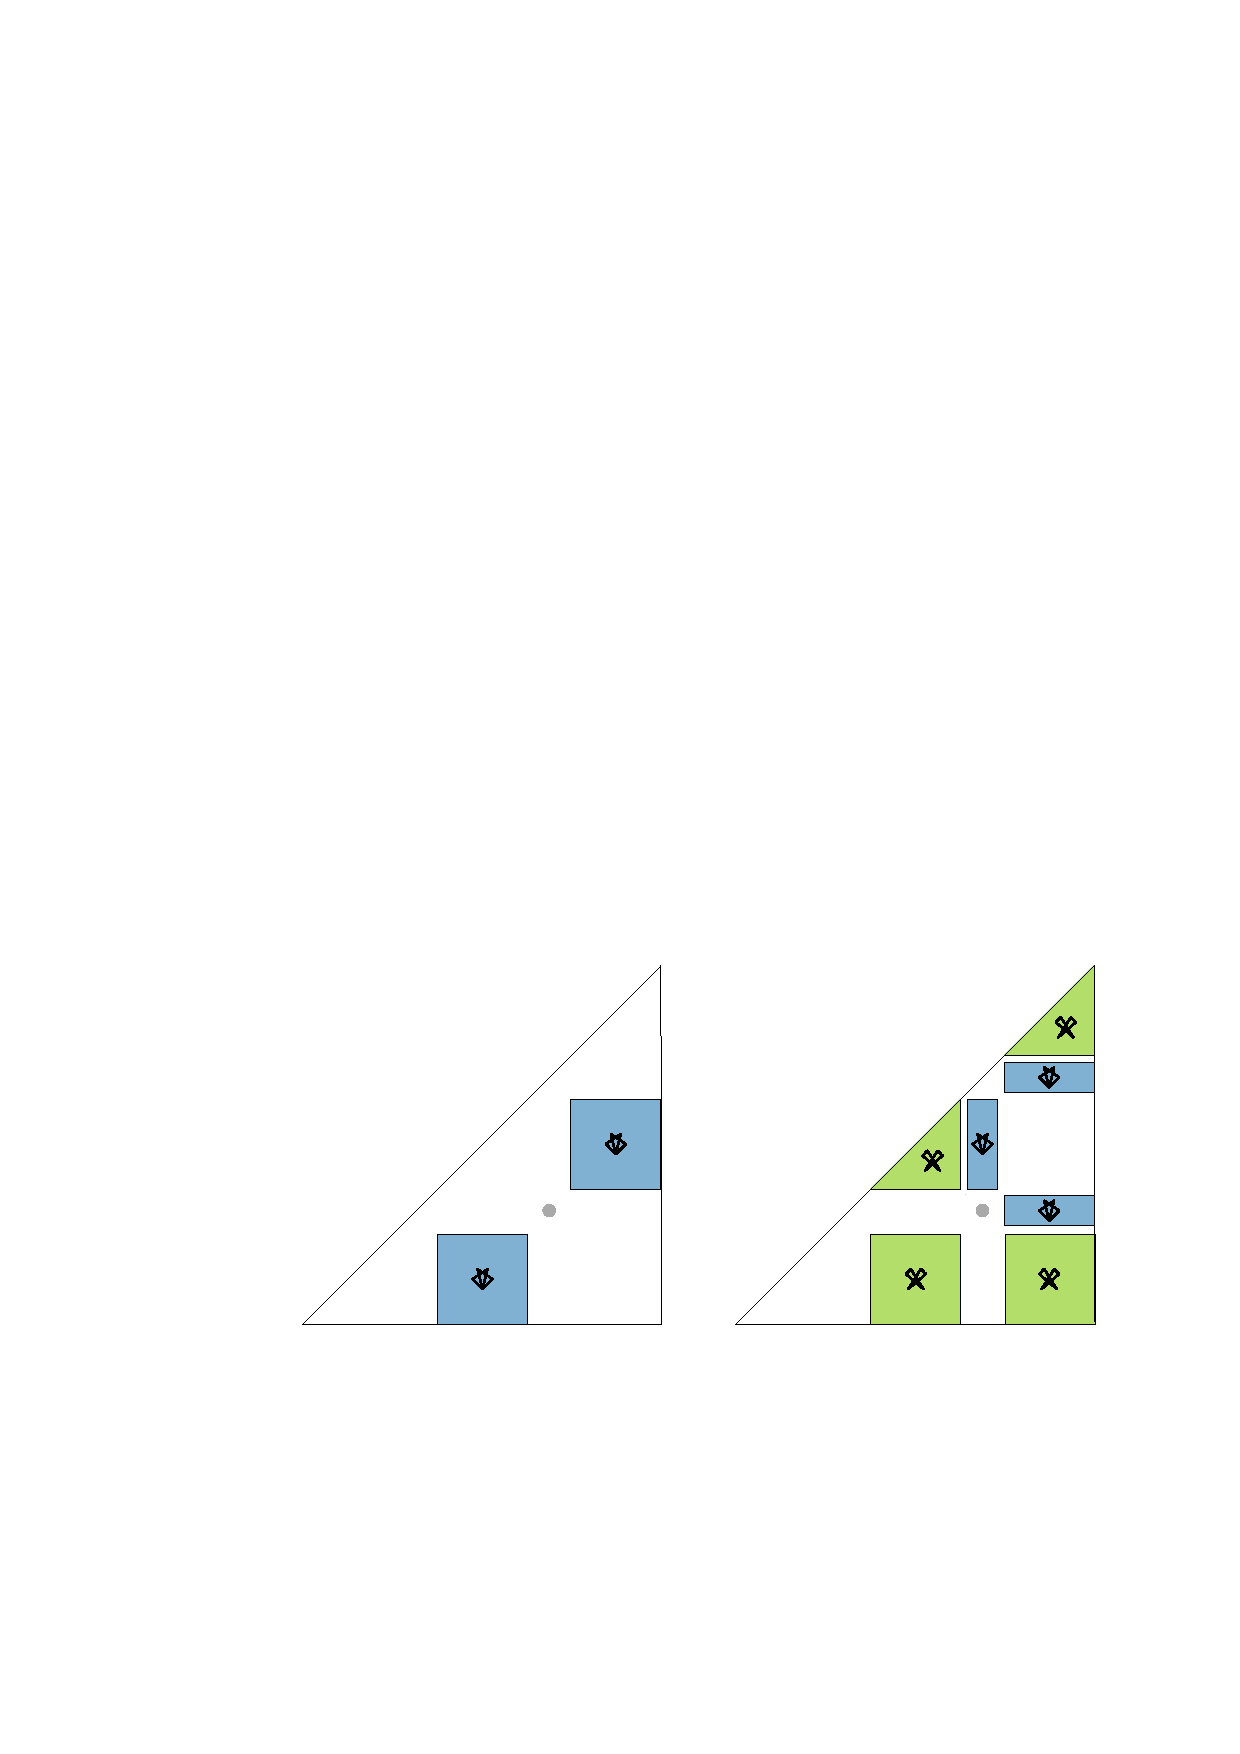
\includegraphics[height=3cm]{figs/helper-8}
\end{center}

\begin{proof}
  The rules for $\crossing$ imply that the points in each $Q_i$ can be
  partitioned into groups $Q_{i,1},\ldots,Q_{i,\ell}$ where the elements
  in $Q_i$ are non-increasing and the elements in $Q_{i,j}$ and $Q_{i,k}$
  do not share any $x$- or $y$-coordinate.  With this observation, the
  rest of the proof is analogous to the proof of \thmref{nested-swords}.
\end{proof}


\subsection{More Linear Upper Bounds}

\begin{thm}\thmlabel{taco-nested-crossing}
  $\ex'(n,\{\taco,\nested,\crossing\}) \in O(n)$.
\end{thm}

\begin{center}
   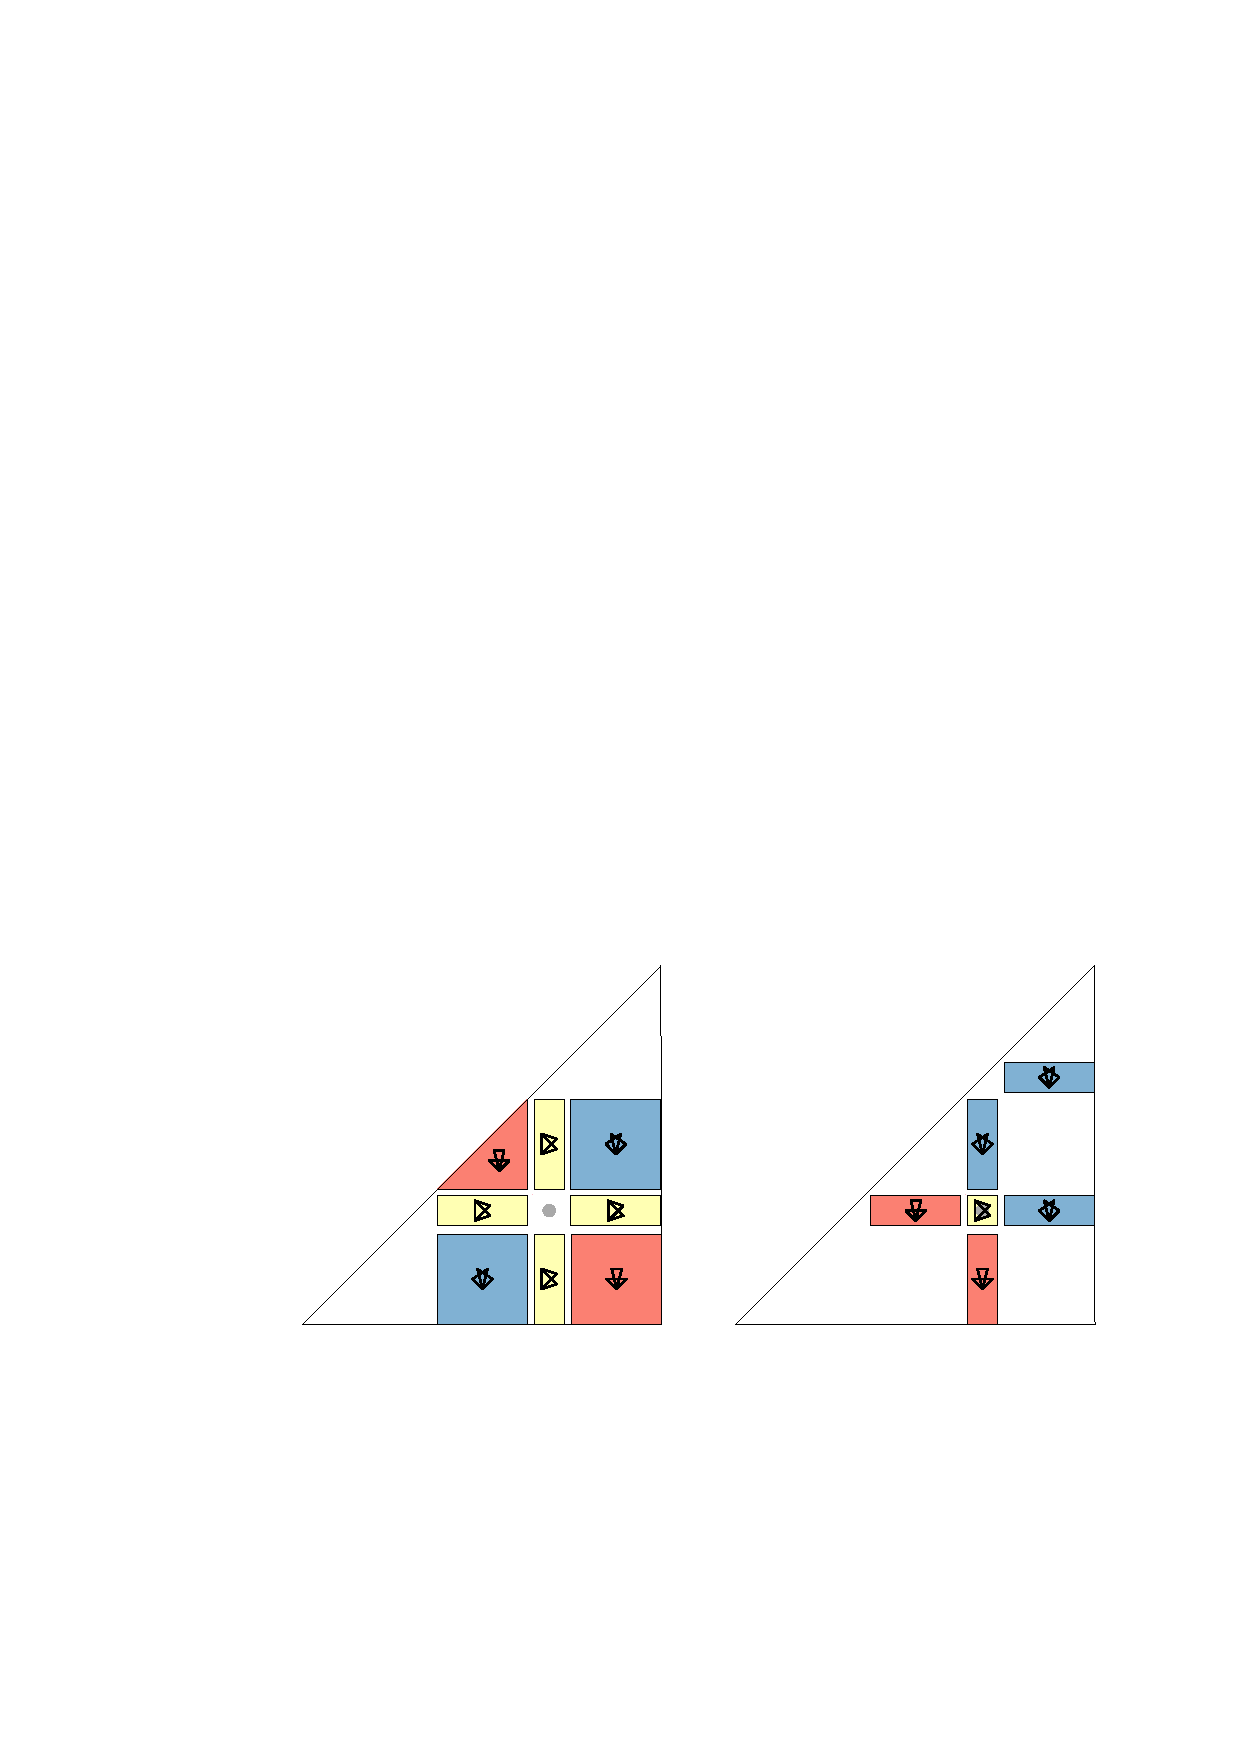
\includegraphics[height=3cm]{figs/helper-9}
\end{center}


\begin{proof}
  Taking the union of the rules for $\taco$, $\nested$, and $\crossing$,
  we obtain the rule which ensures that during subsequent rounds we can
  not take a point from any column or row used in a previous round.
  The rules for $\nested$ and $\taco$ ensure that the set of points
  taken in each $Q_i$ is increasing.  Therefore each new point played
  can be charged to a unique row, so the total number of points played
  is at most $n$.
\end{proof}


\begin{thm}\thmlabel{nested-crossing-ears}
  $\ex'(n,\{\nested,\crossing,\ears\})\in O(n)$.
\end{thm}

\begin{center}
   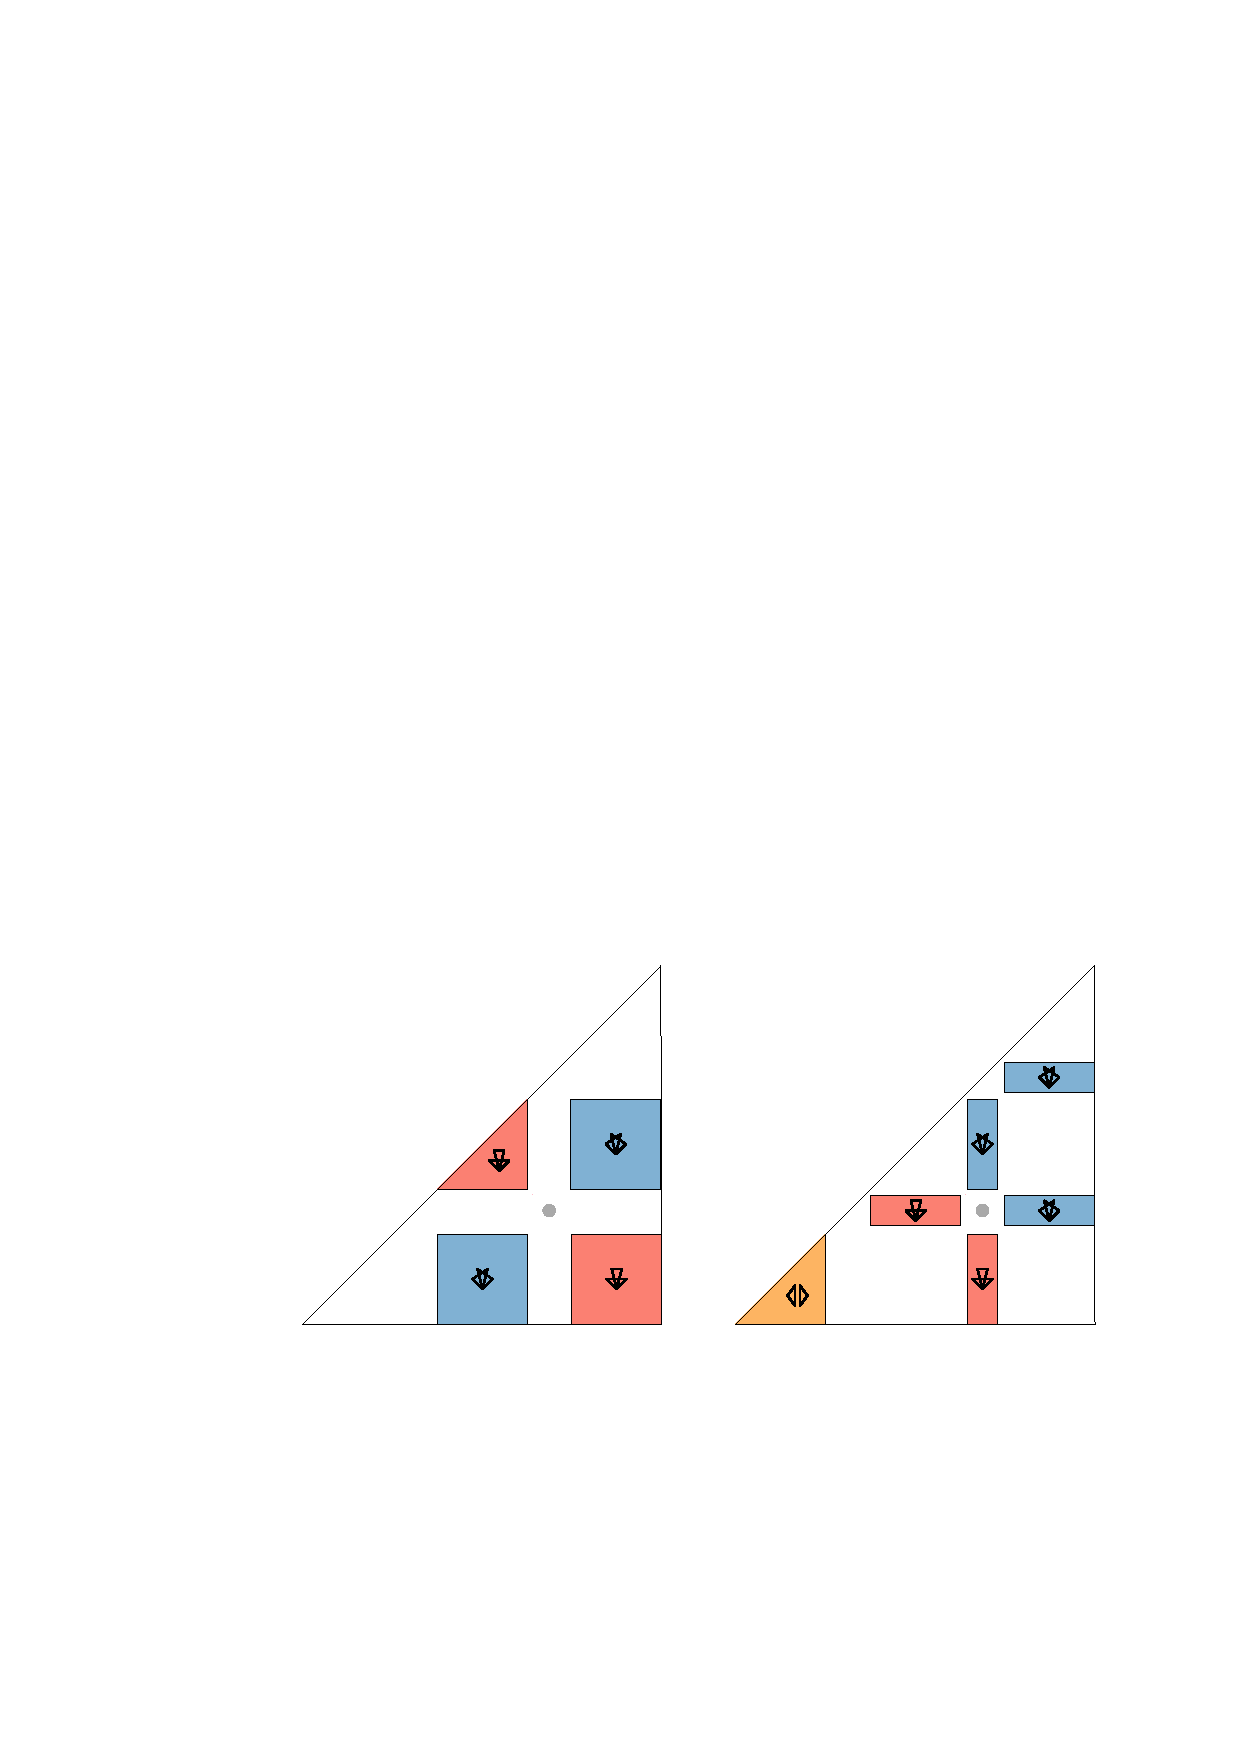
\includegraphics[height=3cm]{figs/helper-10}
\end{center}

\begin{proof}
  First observe that the rules for $\nested$ imply that each $Q_i$
  is a non-decreasing set of points.

  Next, observe that if $Q_i$ contains $k>1$ points in a single column
  (or row), then each of the $k$ rows (or columns) containing one of these
  points is killed, i.e., $Q_{i+1},\ldots,Q_n$ can not contain any points in
  these rows (or columns).  Therefore, when summing $\sum_{i=1}^n |Q_i|$,
  the contribution of points that are not alone in their row or column
  is at most $2n$.  We therefore assume that each $Q_i$ contains at most
  one point from each row and column, which now implies that each $Q_i$
  is an increasing sequence of points.

  Now, because of the rules for $\crossing$, this increasing
  requirement is quite strong. In particular, if we consider the last
  (highest-righmost) point of $Q_i$, then it must be placed so that the
  set of points killed by its $\ears$-region contains all points in $Q_i$
  except itself and the second-last point of $Q_i$.

  To summarize, each row and column of $Q$ contributes at most one point to
  the set
  $S=\bigcup_{i=1}^n Q_i$, so $|S|\le n$.  
  However, the $\ears$-region of the rightmost point in $Q_i$ eliminates
  $|Q_i|-2$ elements of $S$ that can never be played again.  Therefore,
  \[
        n\ge |S| \ge \sum_{i=1}^n (|Q_i|-2) \enspace ,
  \] 
  and we conclude that $\sum_{i=1}^n|Q_i| \le 3n$.
\end{proof}


Our final two upper bounds depend on a simple lemma about forbidden
configurations of points:

\begin{lem}\lemlabel{forbidden}
   Let $S$ be a subset of $\{1,\ldots,n\}^2$ with no three
   points $a=(x_0,y_0)$, $b=(x_0,y_1)$, and $c=(x_1,y_1)$ with $y_0<y_1$
   and $x_0<x_1$.  Then $|S|\le 2n$.
\end{lem}

\begin{proof}
   If we remove the rightmost point from each row of $S$, then each
   column in what remains of $S$ contains at most one point. Otherwise we
   could take $a$ to be the lowest point in a column, $b$ to the highest
   point in the same column, and $c$ to be the missing rightmost point
   in $b$'s row.
\end{proof}

\begin{thm}\thmlabel{taco-nested-david}
  $\ex'(n,\{\taco,\nested,\david\})\in O(n)$.
\end{thm}

\begin{center}
   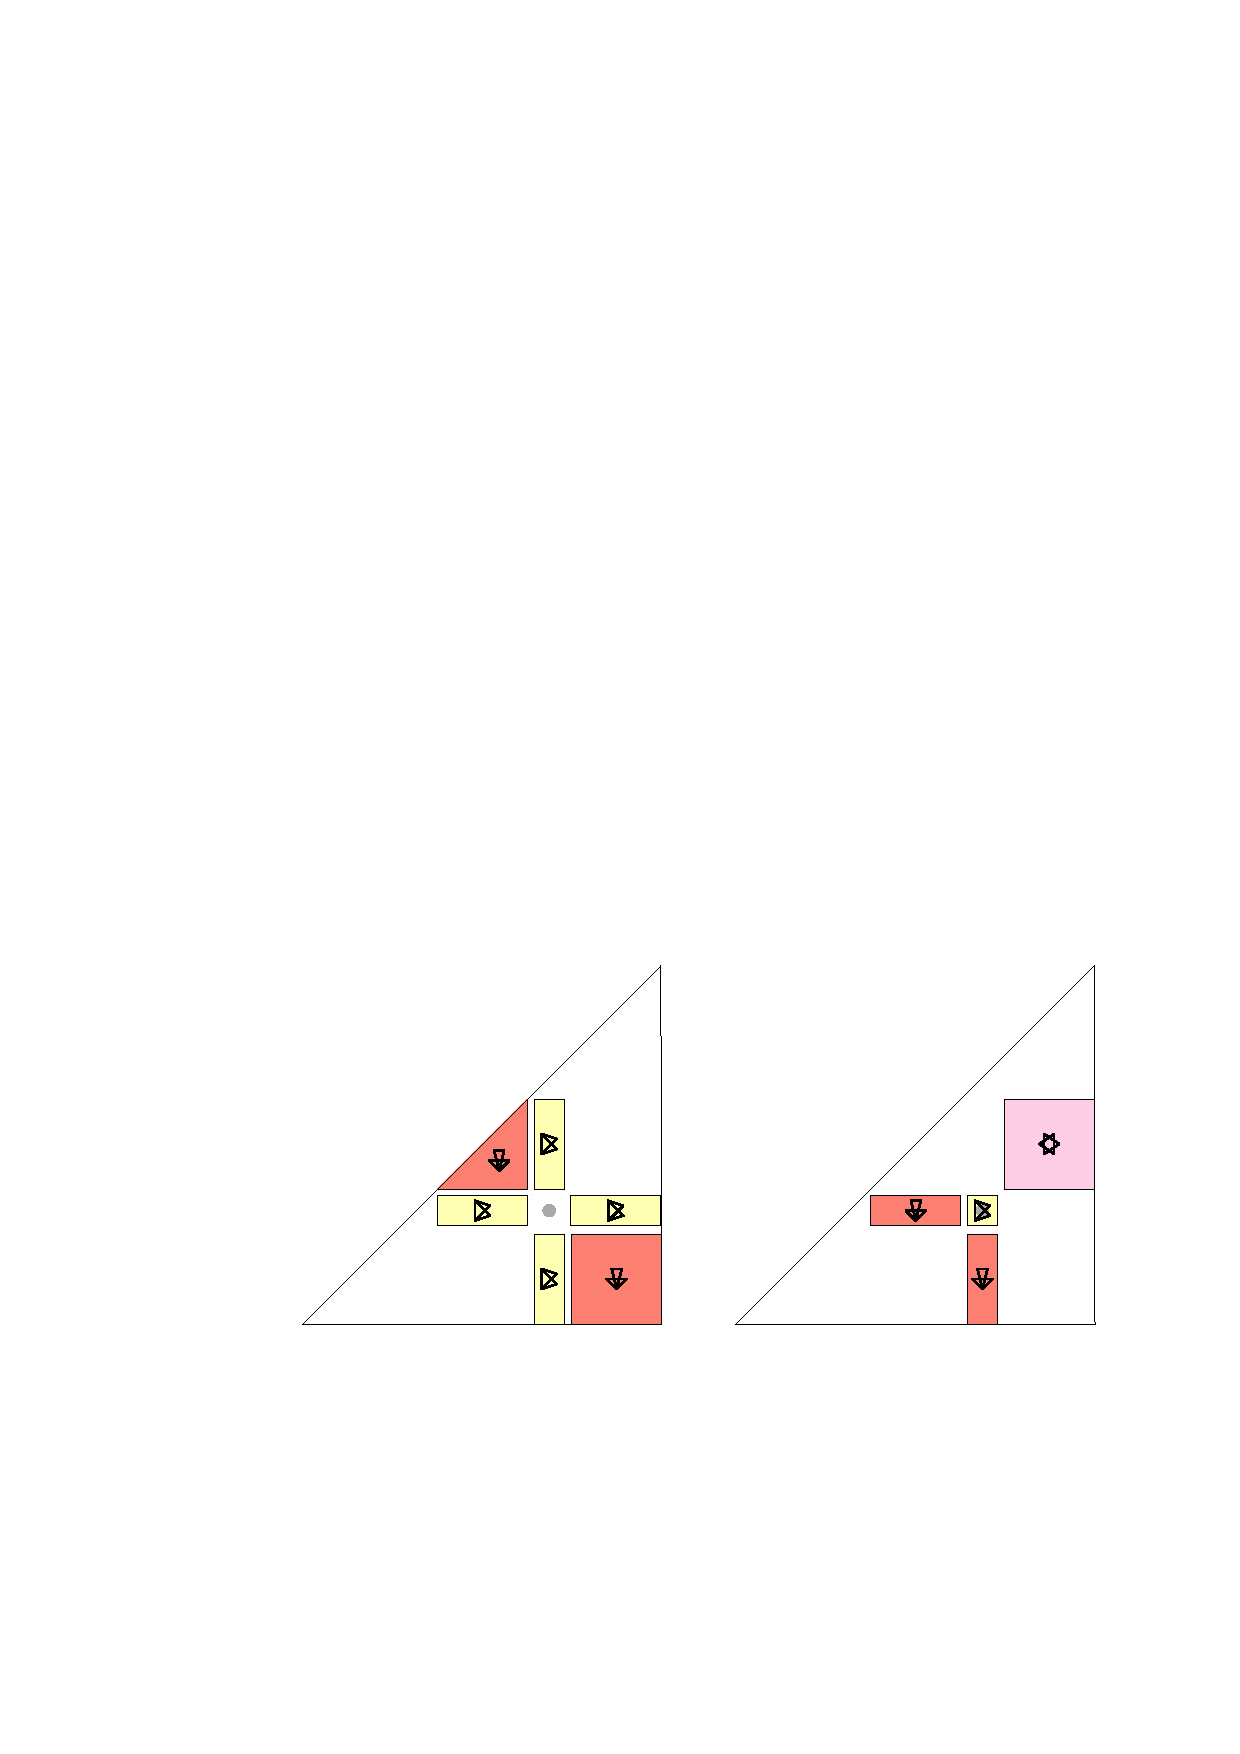
\includegraphics[height=3cm]{figs/helper-11}
\end{center}

\begin{proof}
  Let $S=\bigcup_{i=1}^n Q_i$ be the set of points played in a solution
  to the resulting dot-puzzle.  Note that, by the inclusion of $\taco$,
  each element of $S$ appears in exactly one $Q_i$, so $|S|=\sum_{i=1}^n
  |Q_i|$ is the quantity we are interested in bounding.

  Next, we observe that $S$ does not contain any three points
  $a=(x_0,y_0)$, $b=(x_0,y_1)$, and $c=(x_1,y_1)$ with $y_0<y_1$
  and $x_0<x_1$.  This is because the rules for $\taco$ and $\nested$
  imply that $a$ would have to have been played in a round before $b$,
  and that $b$ would have to have been played in a round before $c$.
  But then the rule for $\david$ implies that $c$ would have to appear
  in a round before $a$.  Applying \lemref{forbidden} then implies that
  $|S|\le 2n$.
\end{proof}


\begin{thm}\thmlabel{nested-bat-david}
  $\ex'(n,\{\nested,\bat,\david\})\in O(n)$.
\end{thm}

\begin{center}
   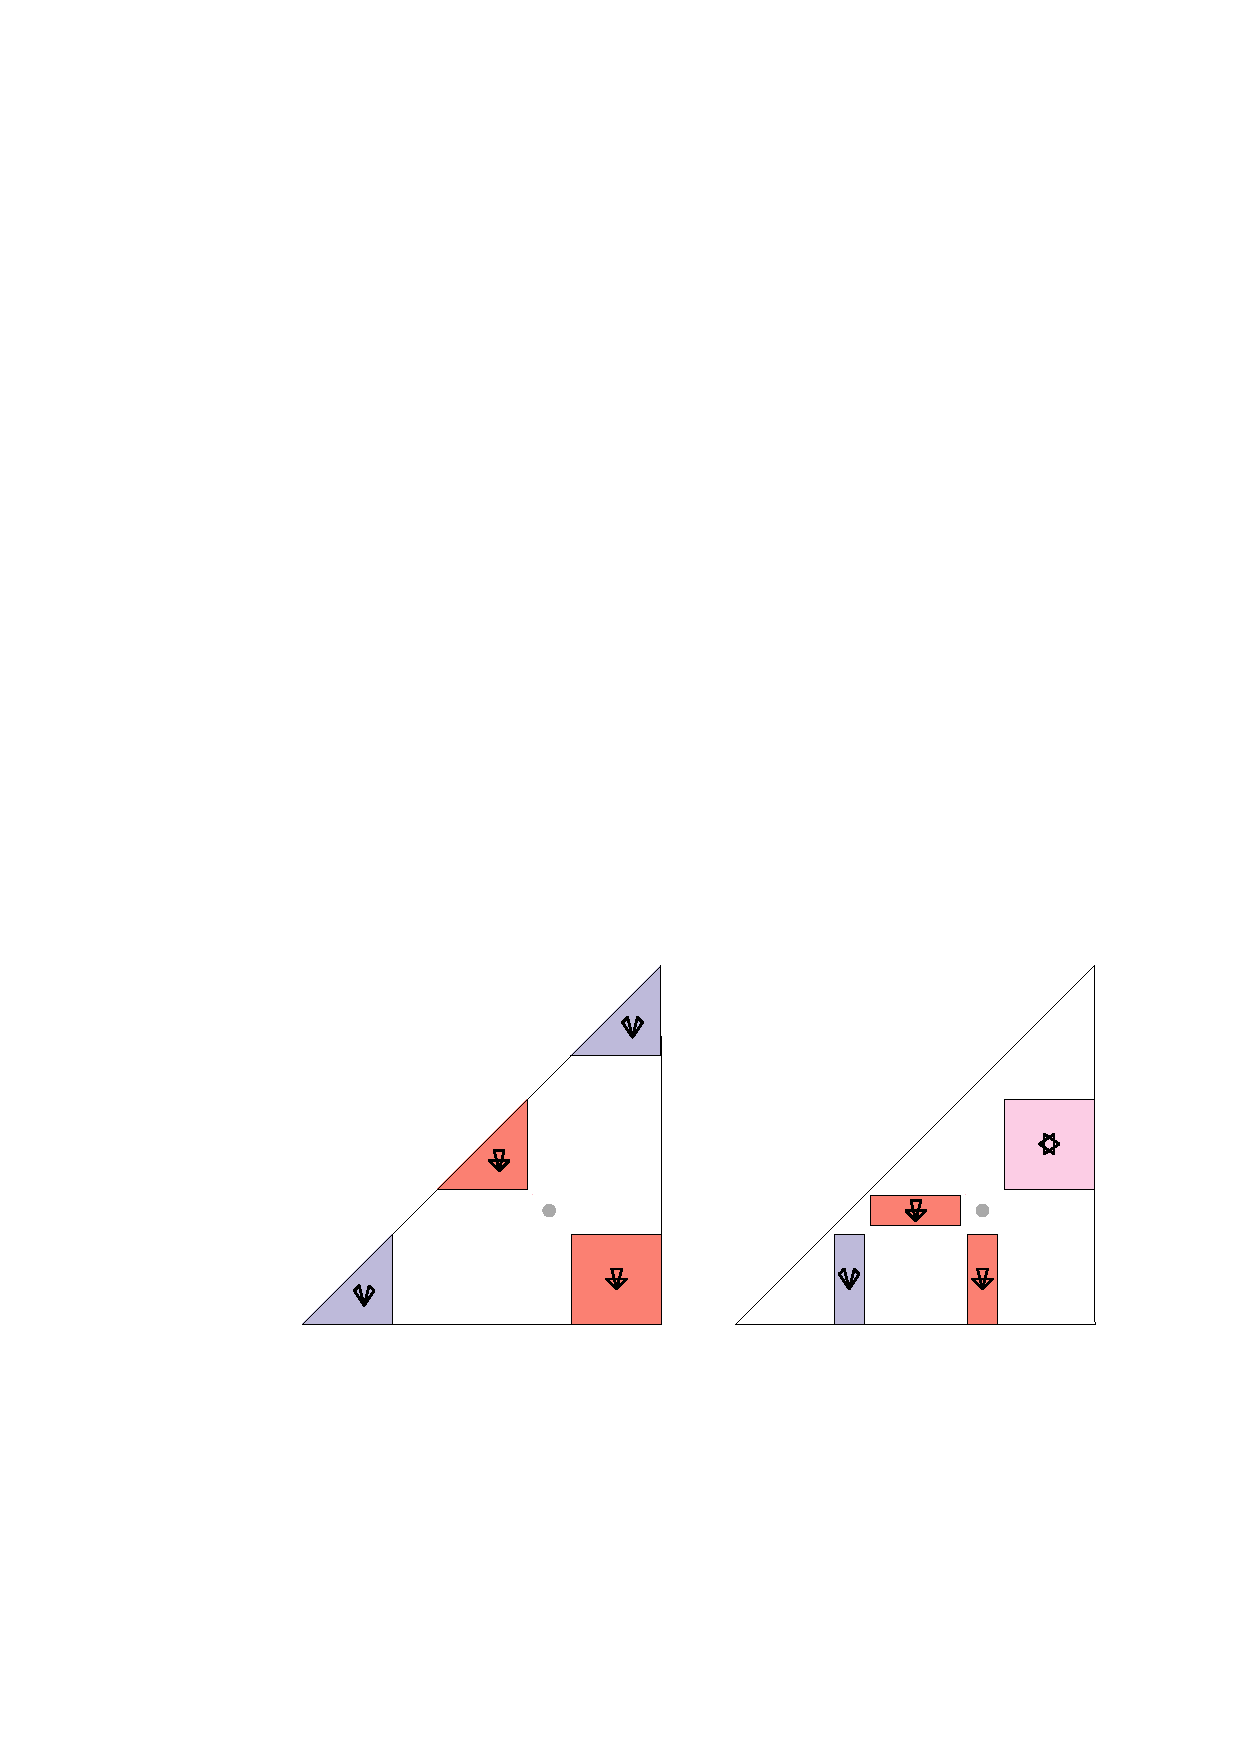
\includegraphics[height=3cm]{figs/helper-12}
\end{center}


\begin{proof}
  Consider the set $Q_i$ played during some round $i$.  The rules for
  $\nested$ imply that $Q_i$ is non-decreasing.  The rule for $\bat$
  implies that $Q_i$ is contained in the $\david$-region, $R_i$, of the
  lowest-leftmost point in $Q_i$.  Indeed, all of $Q_i$ except its
  leftmost row and column is in this $\david$-region.

  Refer to \figref{nested-bat-david}.  Suppose we remove the leftmost
  point in each row of $Q_i$.  For each such point $p\in R_i$, the entire
  row containing $p$ is then killed and can never be played again. The
  only other points we remove are in the first column of $Q_i$ and all
  but two of these (the topmost and bottommost) kill an entire row that
  can never be played again.  This means that the total number of points
  removed this way is not more $3n$ (one charged to each row and two
  charged to each round).  Since $Q_i$ was originally non-decreasing,
  the removal of these points ensures that each column contains at most
  one point of $Q_i$

  \begin{figure}
    \begin{center}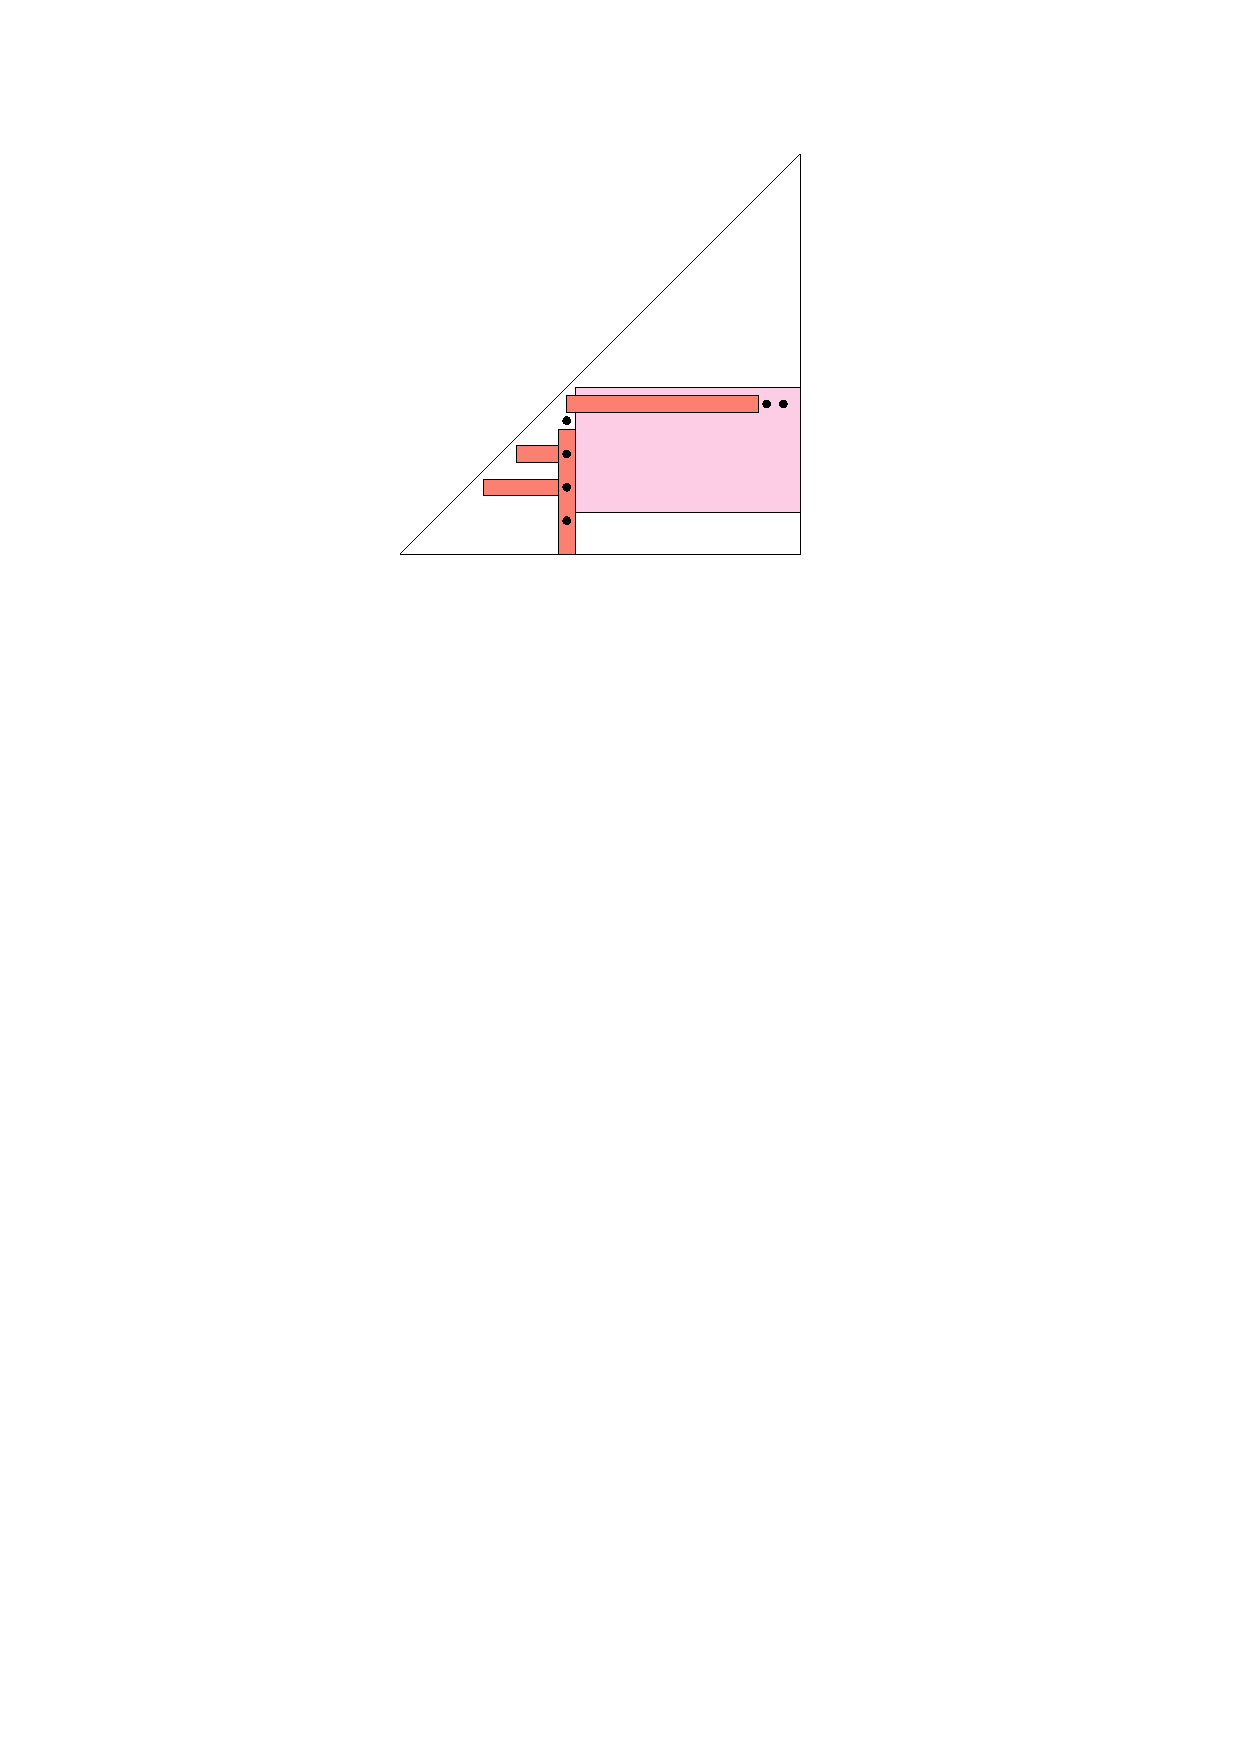
\includegraphics{figs/nested-bat-david}\end{center}
    \caption{The proof of \thmref{nested-bat-david}. The leftmost point
      in each row of $Q_i$ kills an entire row (except possibly for two
      points in the leftmost column).}
    \figlabel{nested-bat-david}
  \end{figure}

  Now we let $S=\bigcup_{i=1}^n Q_i$.  We claim that $S$ fulfills the
  requirements of \lemref{forbidden}.  To see why this is so, note that
  if two points $a$ and $b$ of $S$ are in the same column then they
  must have been played in different rounds.  Assume $b$ is above $a$,
  which implies that $b$ was played in a later round than $a$.  Then, if
  there is some point $c$ to the right of $b$, then $c$ must have been played
  during the same round as $b$ or later.  But this implies that $c$ was
  played in a later round than $a$, which is not possible, since $c$ is in
  $a$'s $\david$-region.  Therefore, by \lemref{forbidden}, $|S|\le 2n$.

  All that remains is to account for points in $S$ that are played
  multiple times.  In each $Q_i$ there are at most two points that can
  be played in subsequent rounds; the topmost point in the leftmost
  column and the rightmost point in the bottom-most row.  We charge each
  occurrence of such repeated points to the rounds in which they are
  the topmost point in the leftmost column and/or the rightmost point
  in the bottommost row.  In this way, each round is charged for at
  most two such points and the total contribution of these points to
  $\sum_{i=1}^n |Q_i|$ is at most $2n$.

  In total, we obtain an upper bound of $7n$ on $\sum_{i=1}^n |Q_i|$.
\end{proof}





\subsection{Monotone Matrices, Tripod Packing, and 2-Comparable Sets}
\seclabel{tripods}

In this section, we discuss $\ex(n,\{\taco,\nested\})$.

\begin{center}
   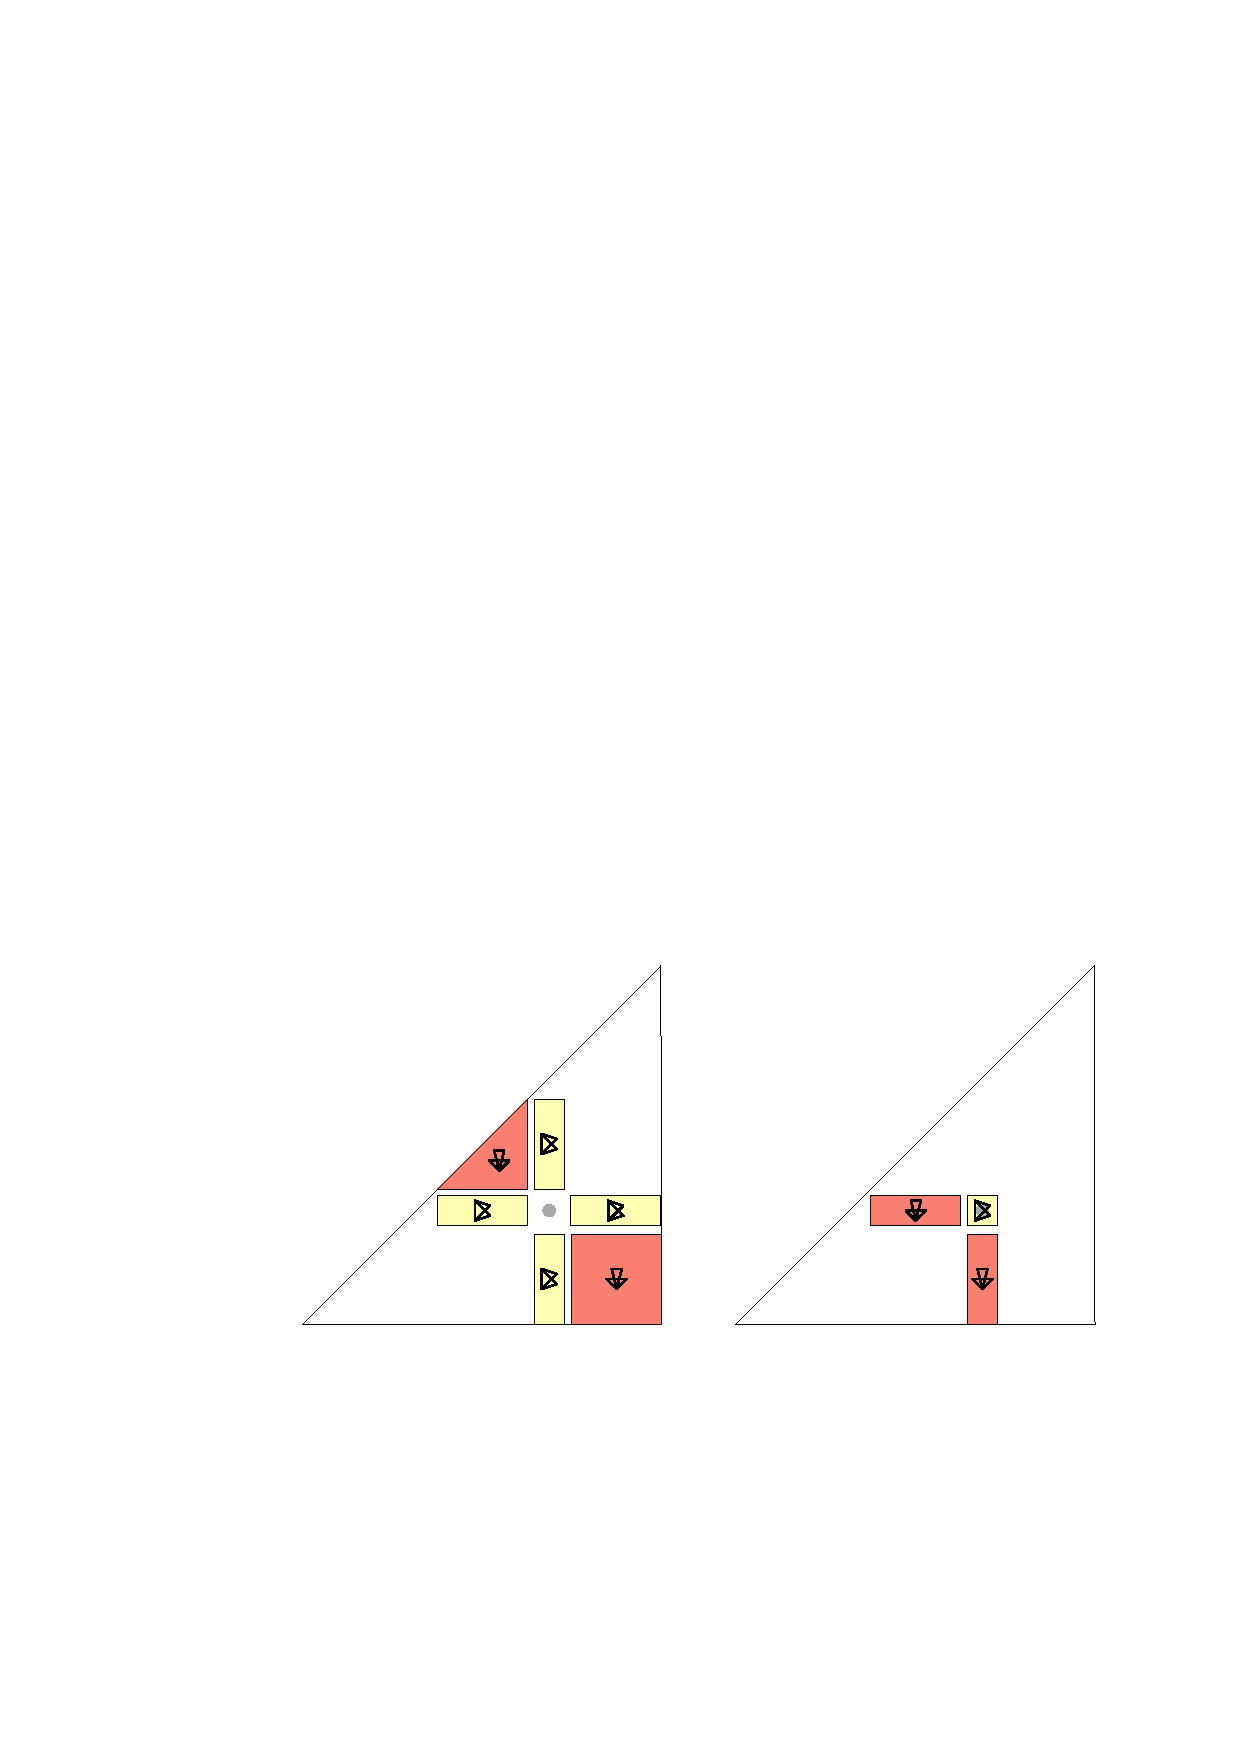
\includegraphics[height=3cm]{figs/helper-13}
\end{center}

Determining the asymptotics of $\ex(n,\{\taco,\nested\})$ was given
explicitly as open problem in the conclusion of Bra\ss's paper.
We spent more than a year work on this problem.  This work included
computer searches for a variant of the problem played on the square grid
$\{1,\ldots,n\}^2$.\footnote{Playing on the square grid does not change
the asympotics of the problem.  Any solution for $\{1,\ldots,n/2\}^2$ can
used as a solution for the triangular grid $Q$ and any upper bound for
$\{1,\ldots,n\}^2$ is also an upper bound for the triangular grid $Q$.}
Using the results of these computer searches in the Online Encyclopedia of
Integer Sequences \cite{oeis:a070214}, we discovered that this problem,
when played on the square grid, is equivalent to several other known
problems. See \figref{tripods}.

\begin{figure}
  \begin{center}
    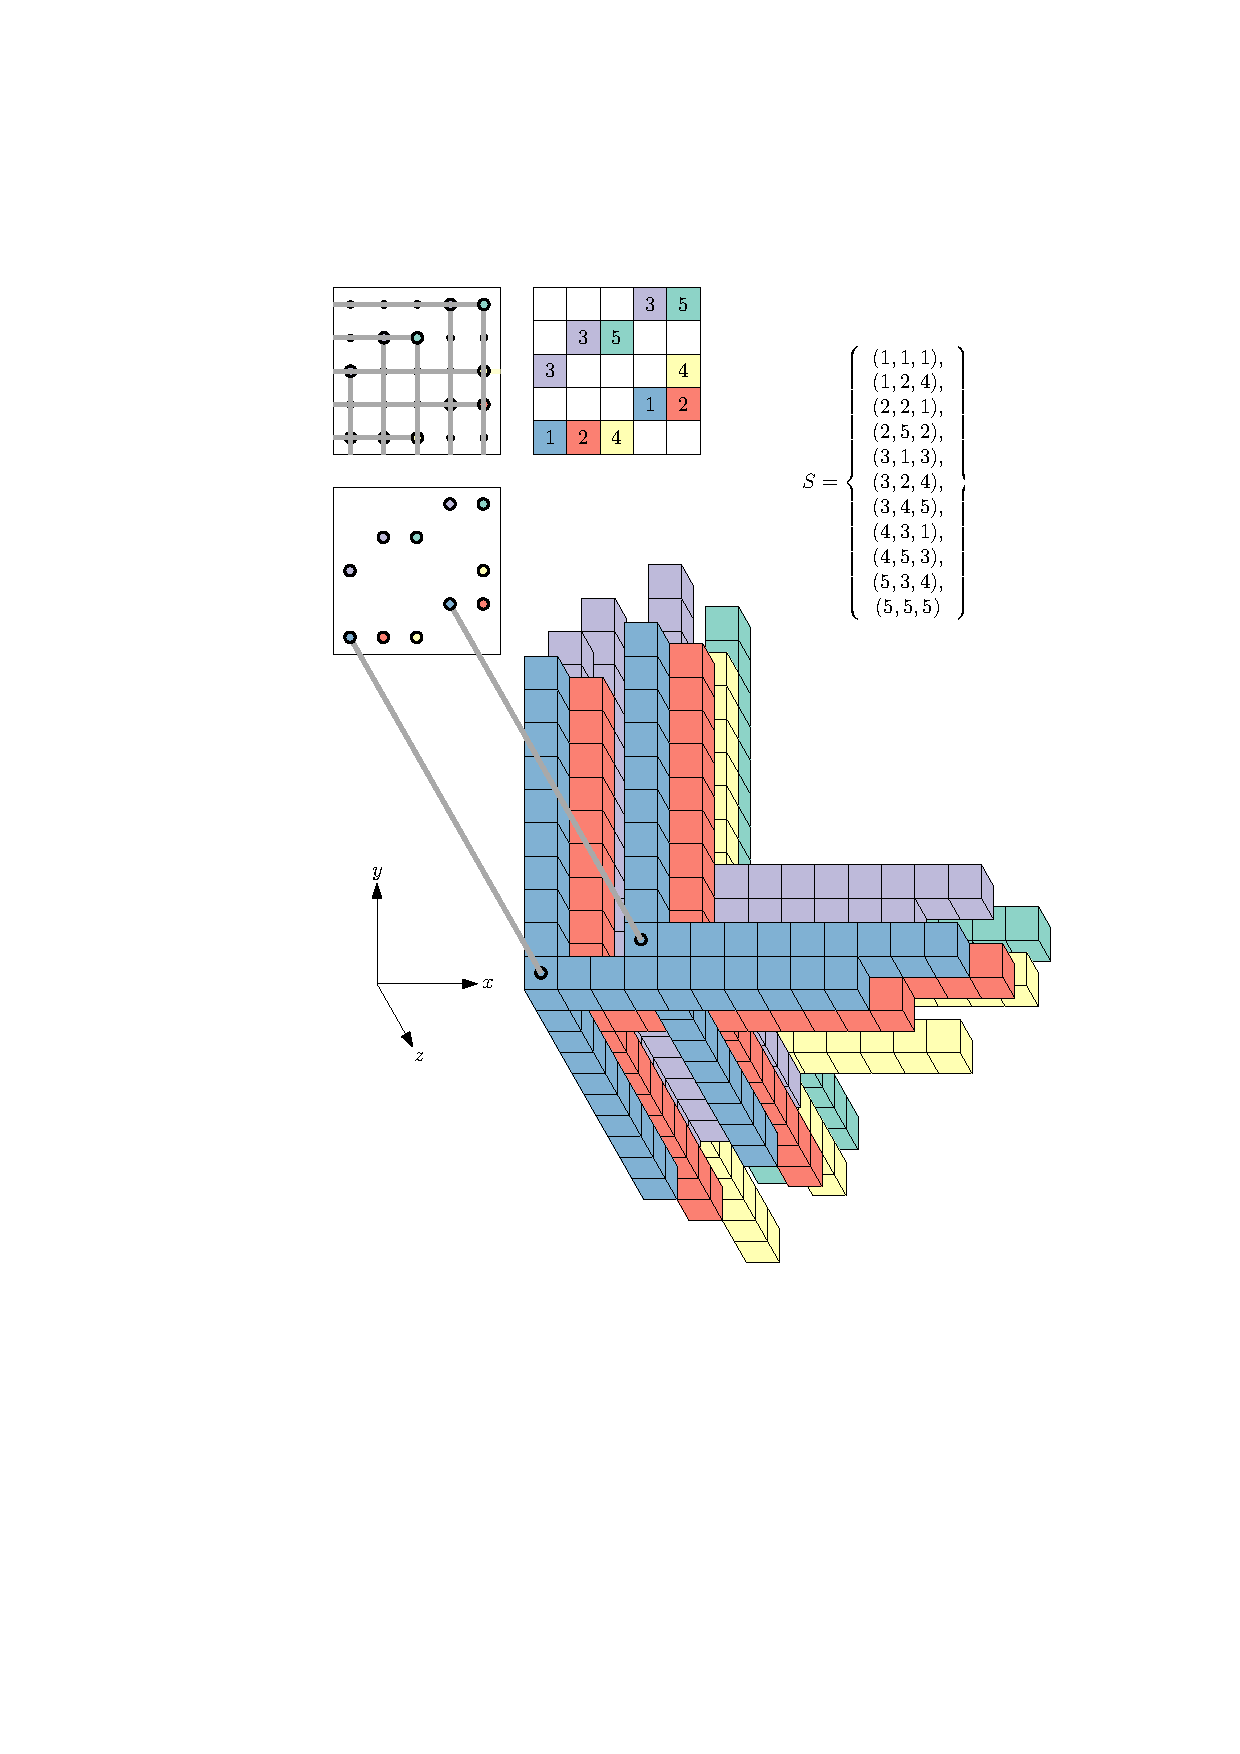
\includegraphics{figs/tripods}
  \end{center}
  \caption{The dot-puzzle induced by excluding the taco and nested configurations
    has already been studied under several equivalent formulations.}
  \figlabel{tripods}
\end{figure}

\begin{enumerate}
  \item \emph{Monotone matrix problem}: How many values from
  $\{1,\ldots,n\}$ can one write in an $n\times n$ matrix so that each
  row is increasing from left-to-right, each column is increasing from
  bottom-to-top, and for each $i\in\{1,\ldots,n\}$, the positions of $i$
  in the matrix form an increasing sequence?

  \item \emph{Tripod packing problem}: A \emph{tripod} with top $p\in\R^3$
  is the union of three closed rays at $p$ and parallel to the $x$-,
  $y$-, and $z$-axes.  How many disjoint tripods can be packed with tops
  in $\{1,\ldots,n\}^3$?

  \item \emph{2-comparable sets of triples problem}.  Two triples of
  integers $(a_1,a_2,a_3)$ and $(b_1,b_2,b_3)$ are \emph{2-comparable}
  if $a_i< b_i$ for at least two values of $i\in\{1,2,3\}$ or $a_i > b_i$
  for at least two values of $i\in\{1,2,3\}$.  What is the largest set,
  $S$, of pairwise 2-comparable triples one can make whose entries come
  from $\{1,\ldots,n\}$?
\end{enumerate}

Several simple and natural construction give lower bounds
of $\Omega(n^{3/2})$ for these problems.  However,
this bound is not tight. A sequence of results using
recursive constructions has steadily raised this lower bound
\cite{gowers.long:length,stein:combinatorial,stein:packing,stein.szabo:algebra,tiskin:packing}.
The current record is held by Gowers and Long \cite{gowers.long:length},
who describe a construction of size $\Omega(n^{1.546})$.

\begin{thm}[Gowers and Long \cite{gowers.long:length}]\thmlabel{taco-nested-lb}
  $\ex'(n,\{\taco,\nested\}) \in \Omega(n^{1.546})$
\end{thm}



The only known upper bounds for this problem come from the fact that a
solution to this problem gives a solution to the Ruzsa-Szemer{\'e}di
induced matching problem \cite{ruzsa.szemeredi:triple}.  
\begin{enumerate}
  \setcounter{enumi}{3}
  \item \emph{Induced-matching problem}: What is the maximum number
  of edges in a bipartite graph $G=(A,B,E)$ with $|A|=|B|=n$ such that
  $E$ can be partitioned in to $n$ \emph{induced matchings} $M_1,\ldots,M_n$?
  That is, each $M_i$ is a matching, and for any two edges $e,f\in M_i$
  there is no edge in $E\setminus\{e,f\}$ that joins an endpoint of $e$
  to an endpoint of $f$.
\end{enumerate}
It is simple to verify that if one takes a 2-comparable set of triples
$S=\{(a_i,b_i,c_i):i\in\{1,\ldots,m\}\}$ then the bipartite graph $G=(A,B,E)$
with $A=B=\{1,\ldots,n\}$ and
  \[
     E = \{ (b_j,c_j): j\in \{1,\ldots,m\}\}
  \]
satisfies the conditions of the induced matching problem, with the
partition into matchings given by
\[
    M_i = \{ (a,b,c)\in E : a = i \} 
\]
Thus, any upper bound for the induced-matching problem an upper bound
on the size of a 2-comparable set of triples.

Upper bounds for the induced matching problem are barely subquadratic,
with the current record being held by Fox's improved version of the
triangle removal lemma \cite{fox:new}, which gives an upper bound
of $n^{2}/e^{\Omega(\log^* n)}$.  See the discussion, for example,
in Gowers and Long \cite{gowers.long:length}.

\begin{thm}[Fox \cite{fox:new}]\thmlabel{taco-nested-ub}
  $\ex'(n,\{\taco,\nested\}) \in n^2/e^{\Omega(\log^* n)}$
\end{thm}

While discovering these results, we noticed that the relationships
between some of these problems have gone unnoticed.  Here we point out
a few bibliographic notes:

\begin{itemize}
  \item  Bra\ss\ \cite{brass:turan} seems to have been unaware that
  the question he posed was equivalent to tripod packing and monotone
  matrices (or, like us, had never heard of these problems).
  
  \item Tiskin \cite{tiskin:packing}, apparently unaware of the
  relation between tripod packing and induced matchings, proved an upper
  bound of $o(n^2)$ for tripod packing. His proof does not depend on any
  properties of tripod packing that are not also true for induced matchings,
  and uses the same tools
  (namely Szemeredi's Regularity Lemma) as the original upper bounds for
  the induced matching problem.

  \item Gowers and Long \cite{gowers.long:length} seem to be unaware
  that the problem on 2-comparable sets of triples was studied under
  other names.
  
  \item Gowers and Long \cite{gowers.long:length} arrived at 2-comparable
  sets as a relaxation of a problem (the size of the largest 2-increasing
  sequence of triples)  proposed by Loh \cite{loh:directed}.  In his
  discussion of this problem, Loh formulates a restricted version of the
  induced matching problem, in which the matching must satisfy a certain
  $\Sigma$-free property and expresses hope \cite[Remark~9]{loh:directed}
  that this restricted version has an $O(n^{3/2})$ upper bound.  However,
  solutions for tripod packing correspond to $\Sigma$-free induced
  matchings, so $\Sigma$-free induced matchings of size $\omega(n^{3/2})$
  are already known.
\end{itemize}


In our context, the only new observation we have pertains to
$\ex'(n,\{\taco,\nested,\bat,\ears\})$.
\begin{center}
   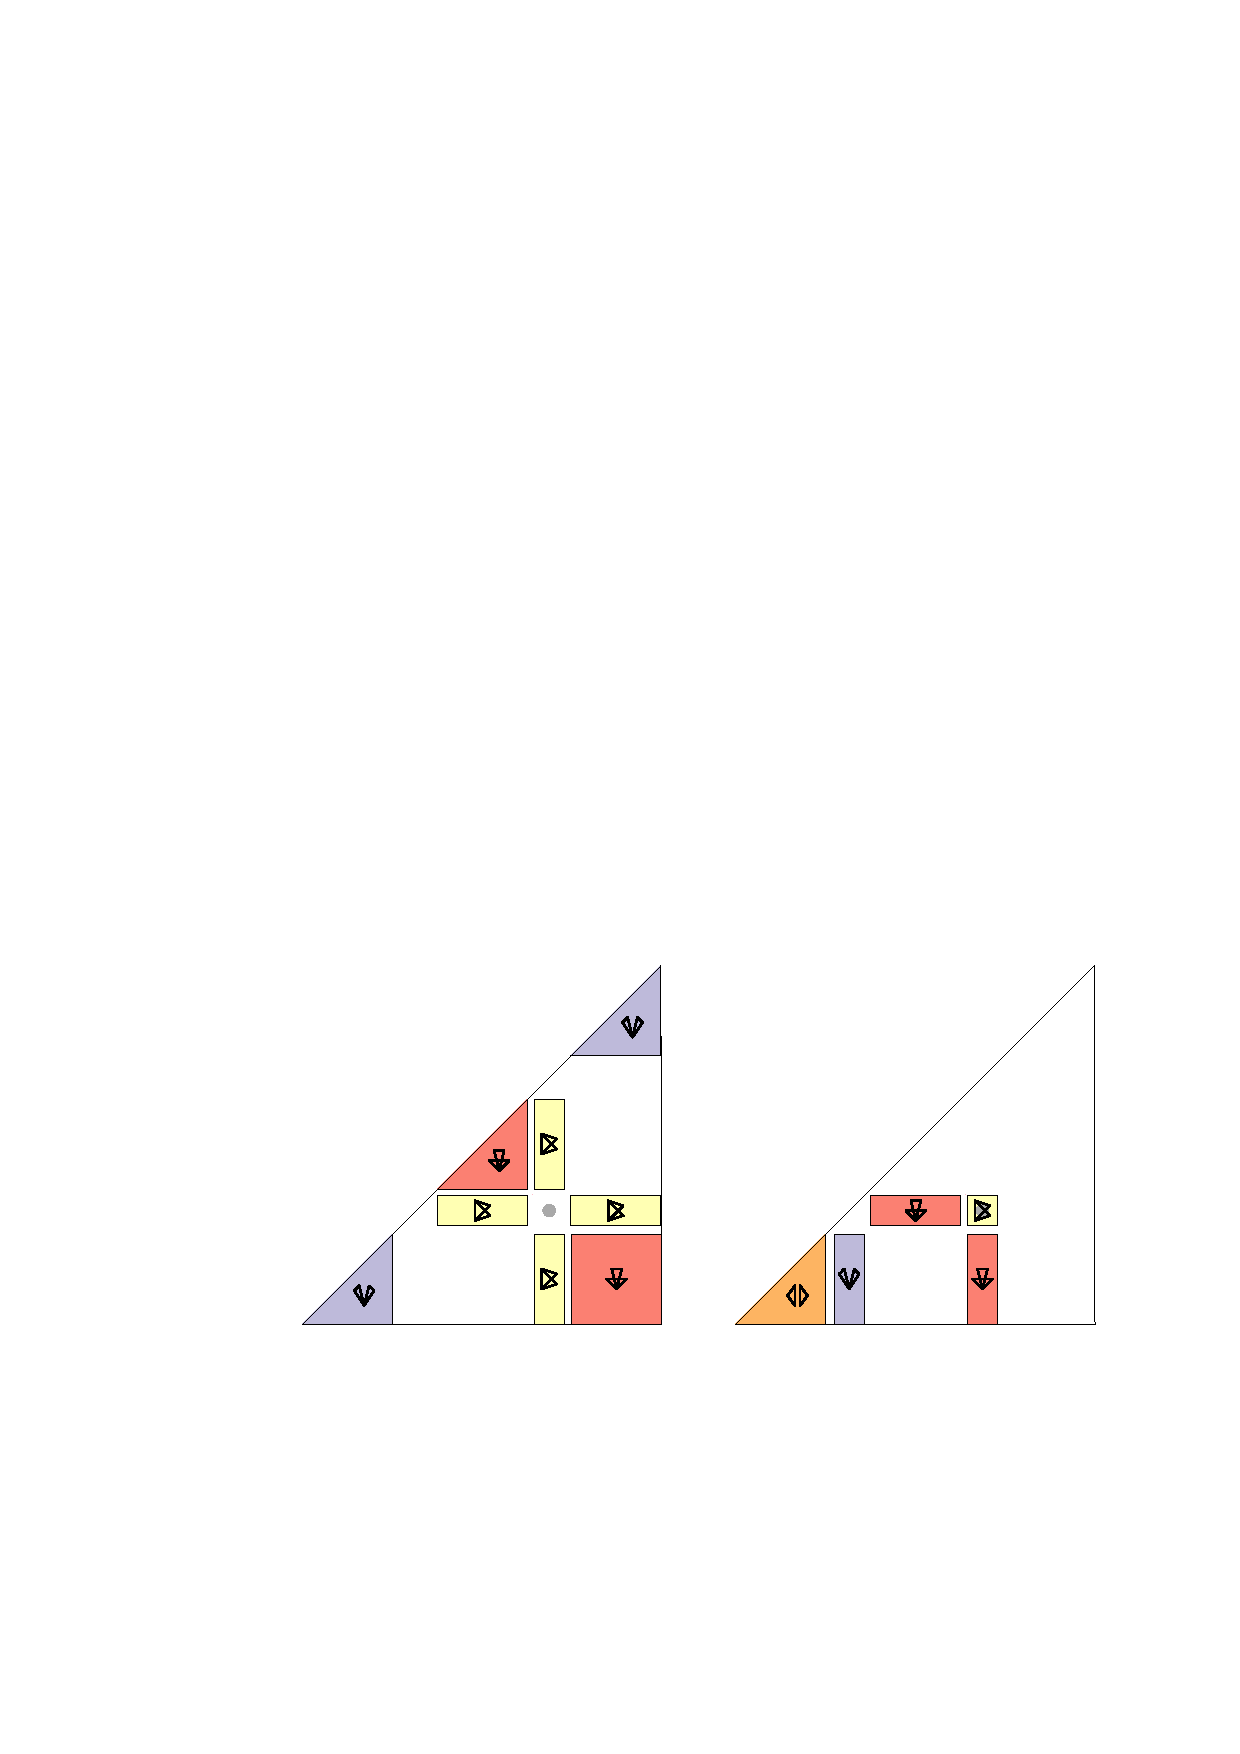
\includegraphics[height=3cm]{figs/helper-14}
\end{center}
We observe that $\ex'(n,\{\taco,\nested\})\in
O(\ex'(n,\{\taco,\nested,\bat,\ears\})$ so these two functions
therefore have the same asymptotic growth.  This comes from the
fact that a solution for the dot-puzzle of size $n$ resulting from
$X=\{\taco,\nested\}$ can be used as a solution for the dot-puzzle of size
$2(n+1)$ resulting from $X=\{\taco,\nested,\bat,\ears\}$ by only playing
in the lower-right quadrant.  When played this way, the extra restrictions
caused by $\bat$ and $\ears$ do not affect the lower-right quadrant.

\begin{thm}
   $\ex'(n,\{\taco,\nested\}) \in \Theta(\ex'(n,\{\taco,\nested,\bat,\ears\})$  
\end{thm}

\subsection{Lower Bounds}
\seclabel{lower-bounds}

Finally, we clean up with some $\Omega(n^2)$ lower bound constructions.
In each case, a matching upper bound follows from one of the results in
Bra\ss \cite{brass:turan}.

\begin{thm}\thmlabel{taco-david-bat-ears}
$\ex(n,\{\taco,\david,\crossing,\bat,\ears\})\in\Theta(n^2)$.
\end{thm}

\begin{center}
   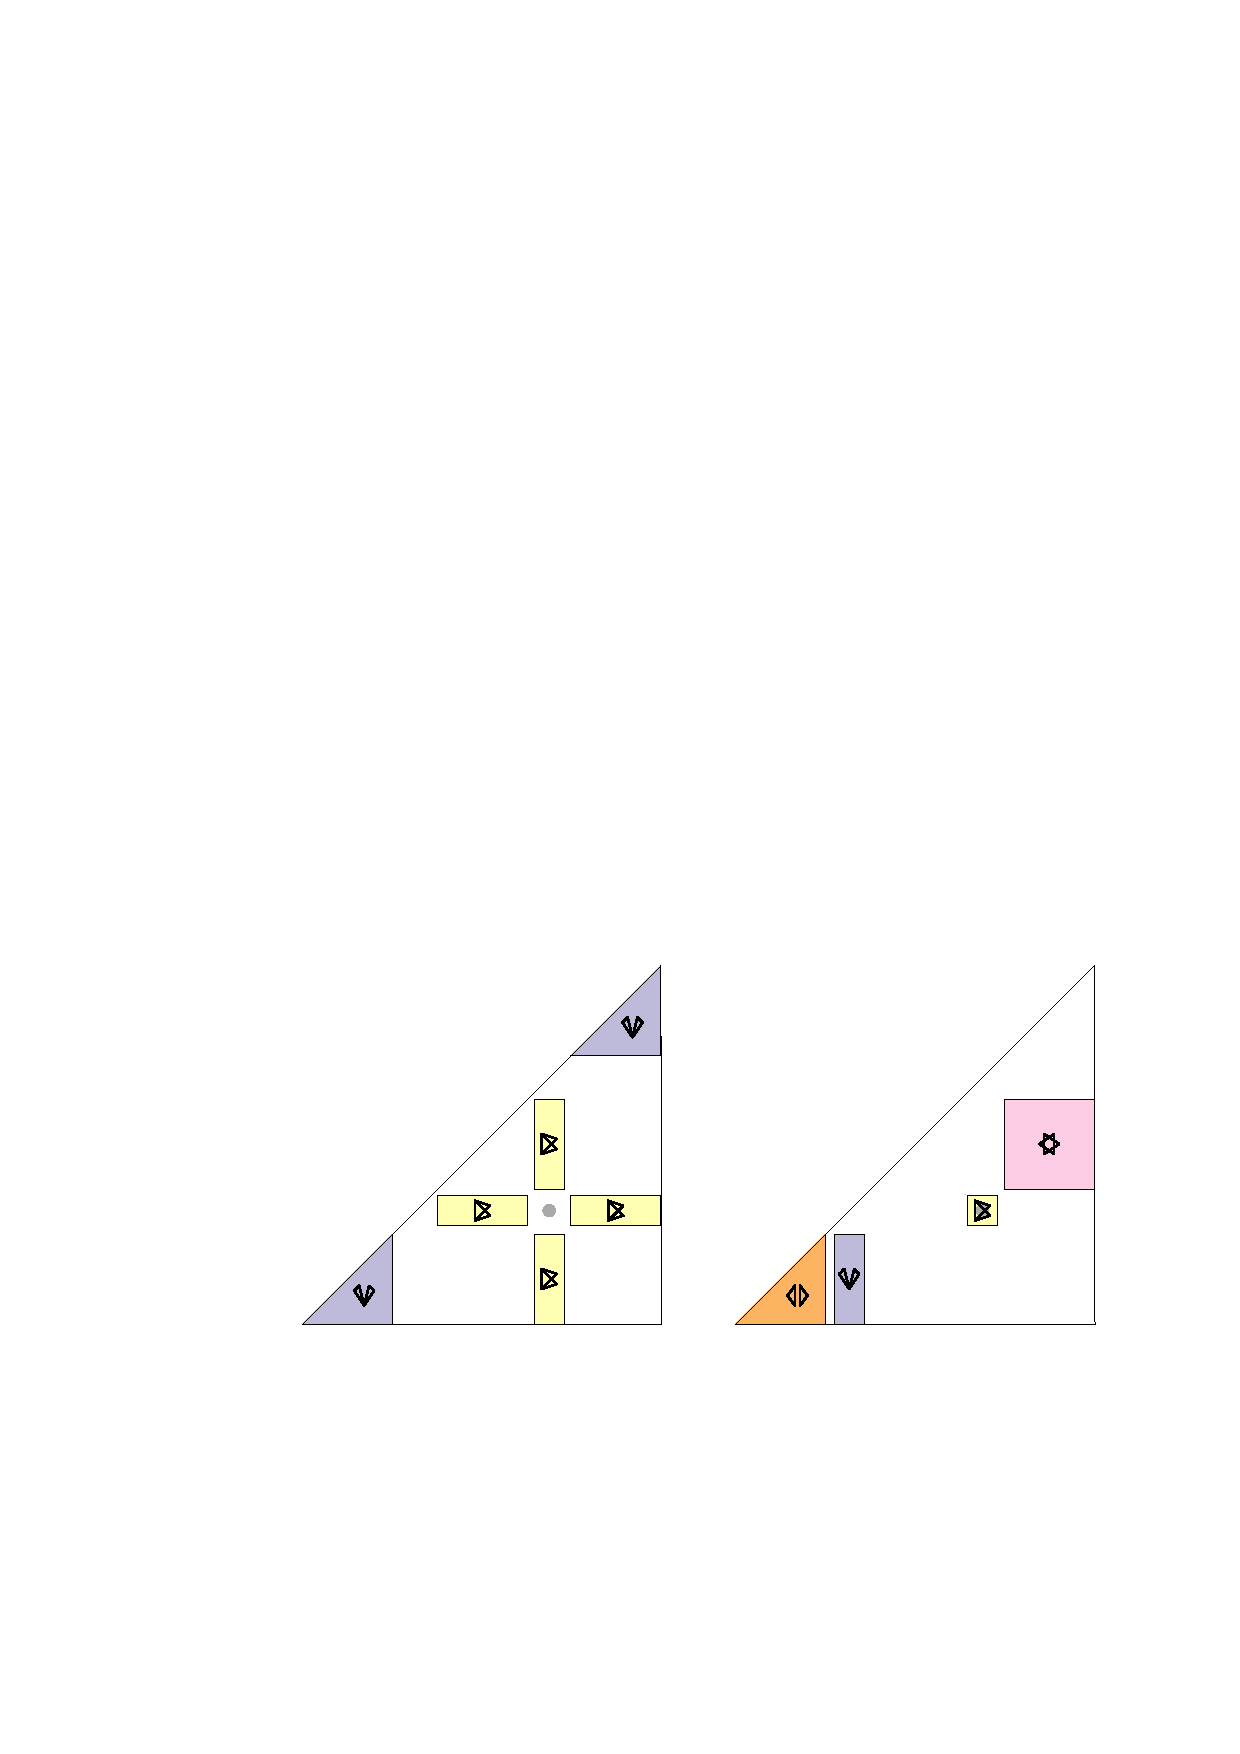
\includegraphics[height=3cm]{figs/helper-15}
\end{center}

\begin{proof}
We set $Q_i$ to be all the points of $\{n/2,\ldots,n\}^2$ on the line $y=n-x-i$.
\end{proof}

\begin{thm}\thmlabel{swords-bat-ears-david}
  $\ex(n,\{\swords,\bat,\ears,\david\}) \in \Theta(n^2)$.
\end{thm}
\begin{center}
   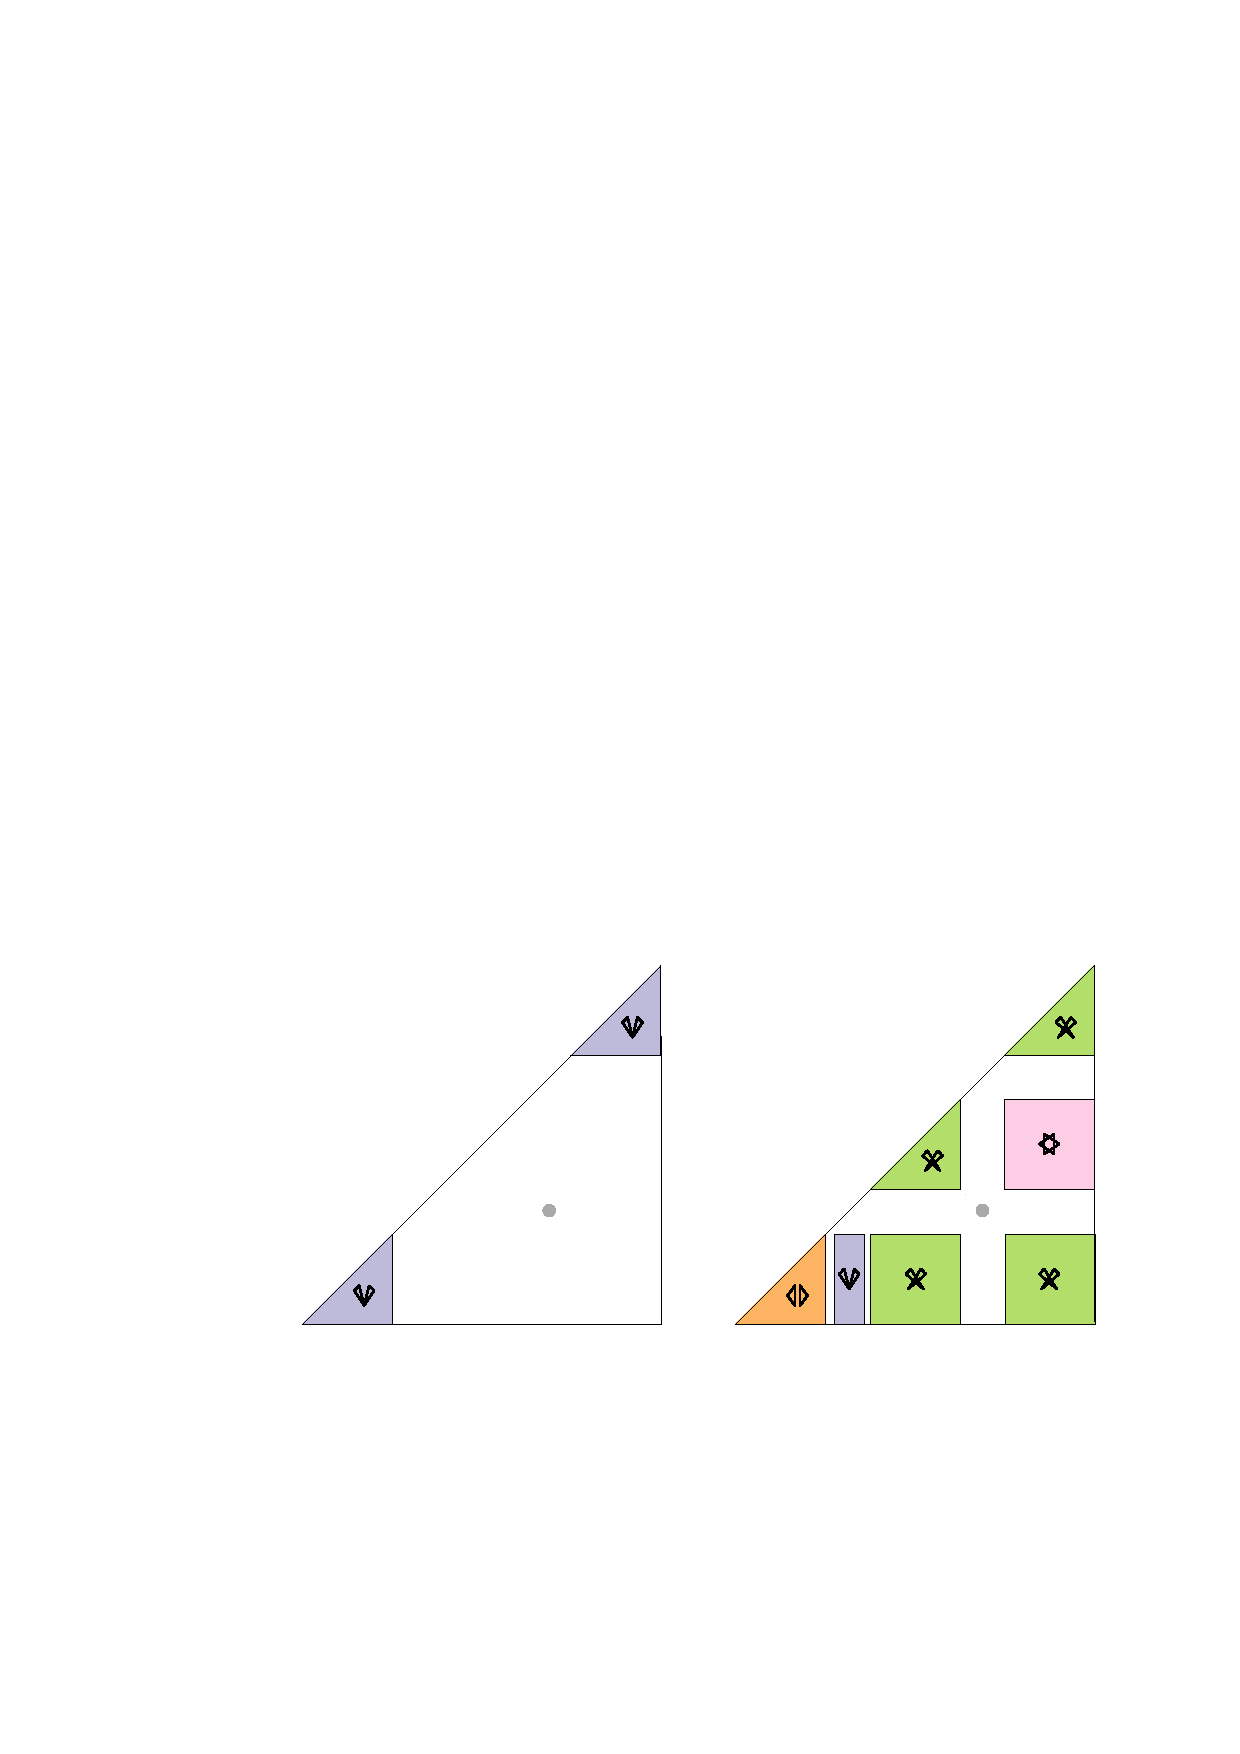
\includegraphics[height=3cm]{figs/helper-16}
\end{center}


\begin{proof}
   We set $Q_1=\{(x,y)\in Q: x>n/2, y<n/2\}$ and
   set $Q_2=Q_3=\cdots Q_n=\emptyset$.
\end{proof}

\begin{thm}\thmlabel{nested-ears-david}
  $\ex(n,\{\nested,\ears,\david\}) \in \Theta(n^2)$.
\end{thm}
\begin{center}
   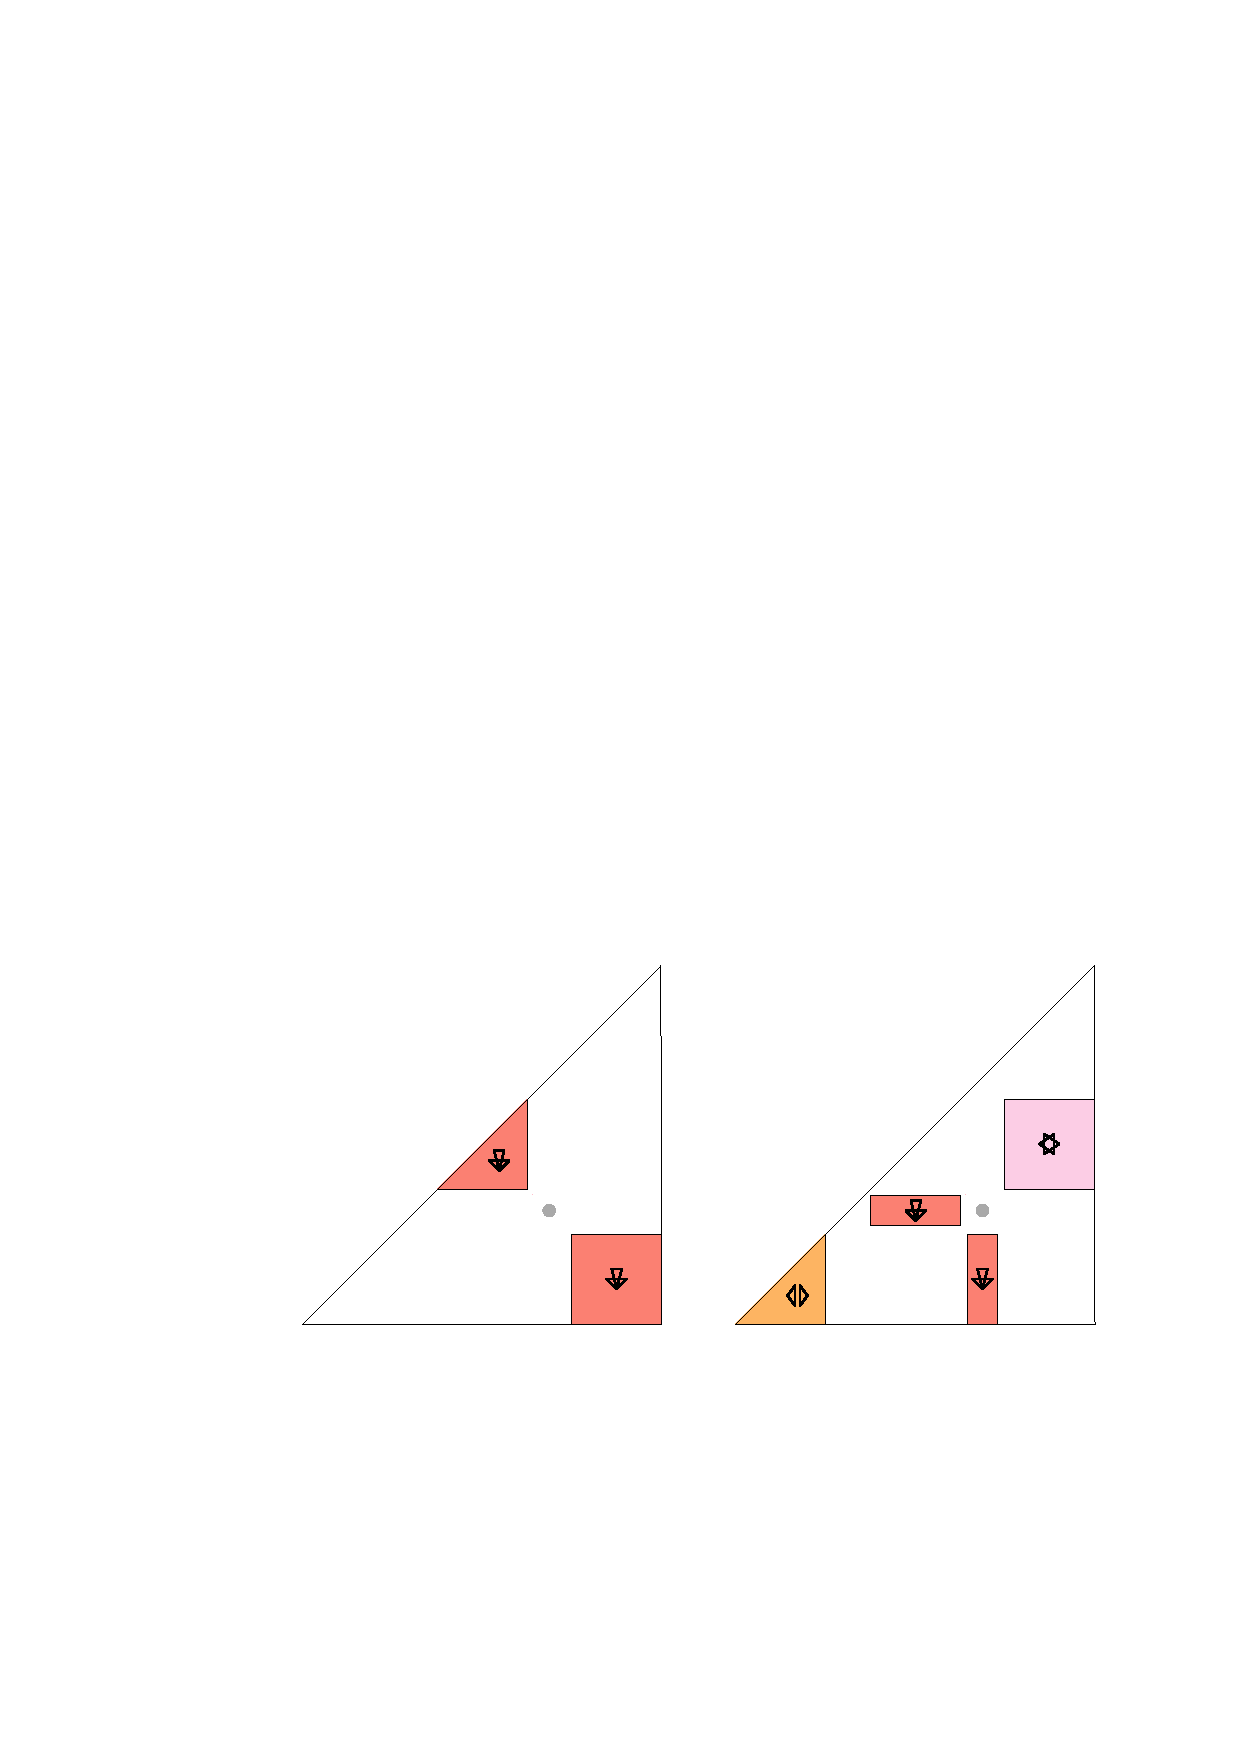
\includegraphics[height=3cm]{figs/helper-17}
\end{center}


\begin{proof}
   Keep taking the bottom row.
\end{proof}

\begin{thm}\thmlabel{david-nested-crossing}
  $\ex(n,\{\david,\nested,\crossing\}) \in \Theta(n^2)$.
\end{thm}
\begin{center}
   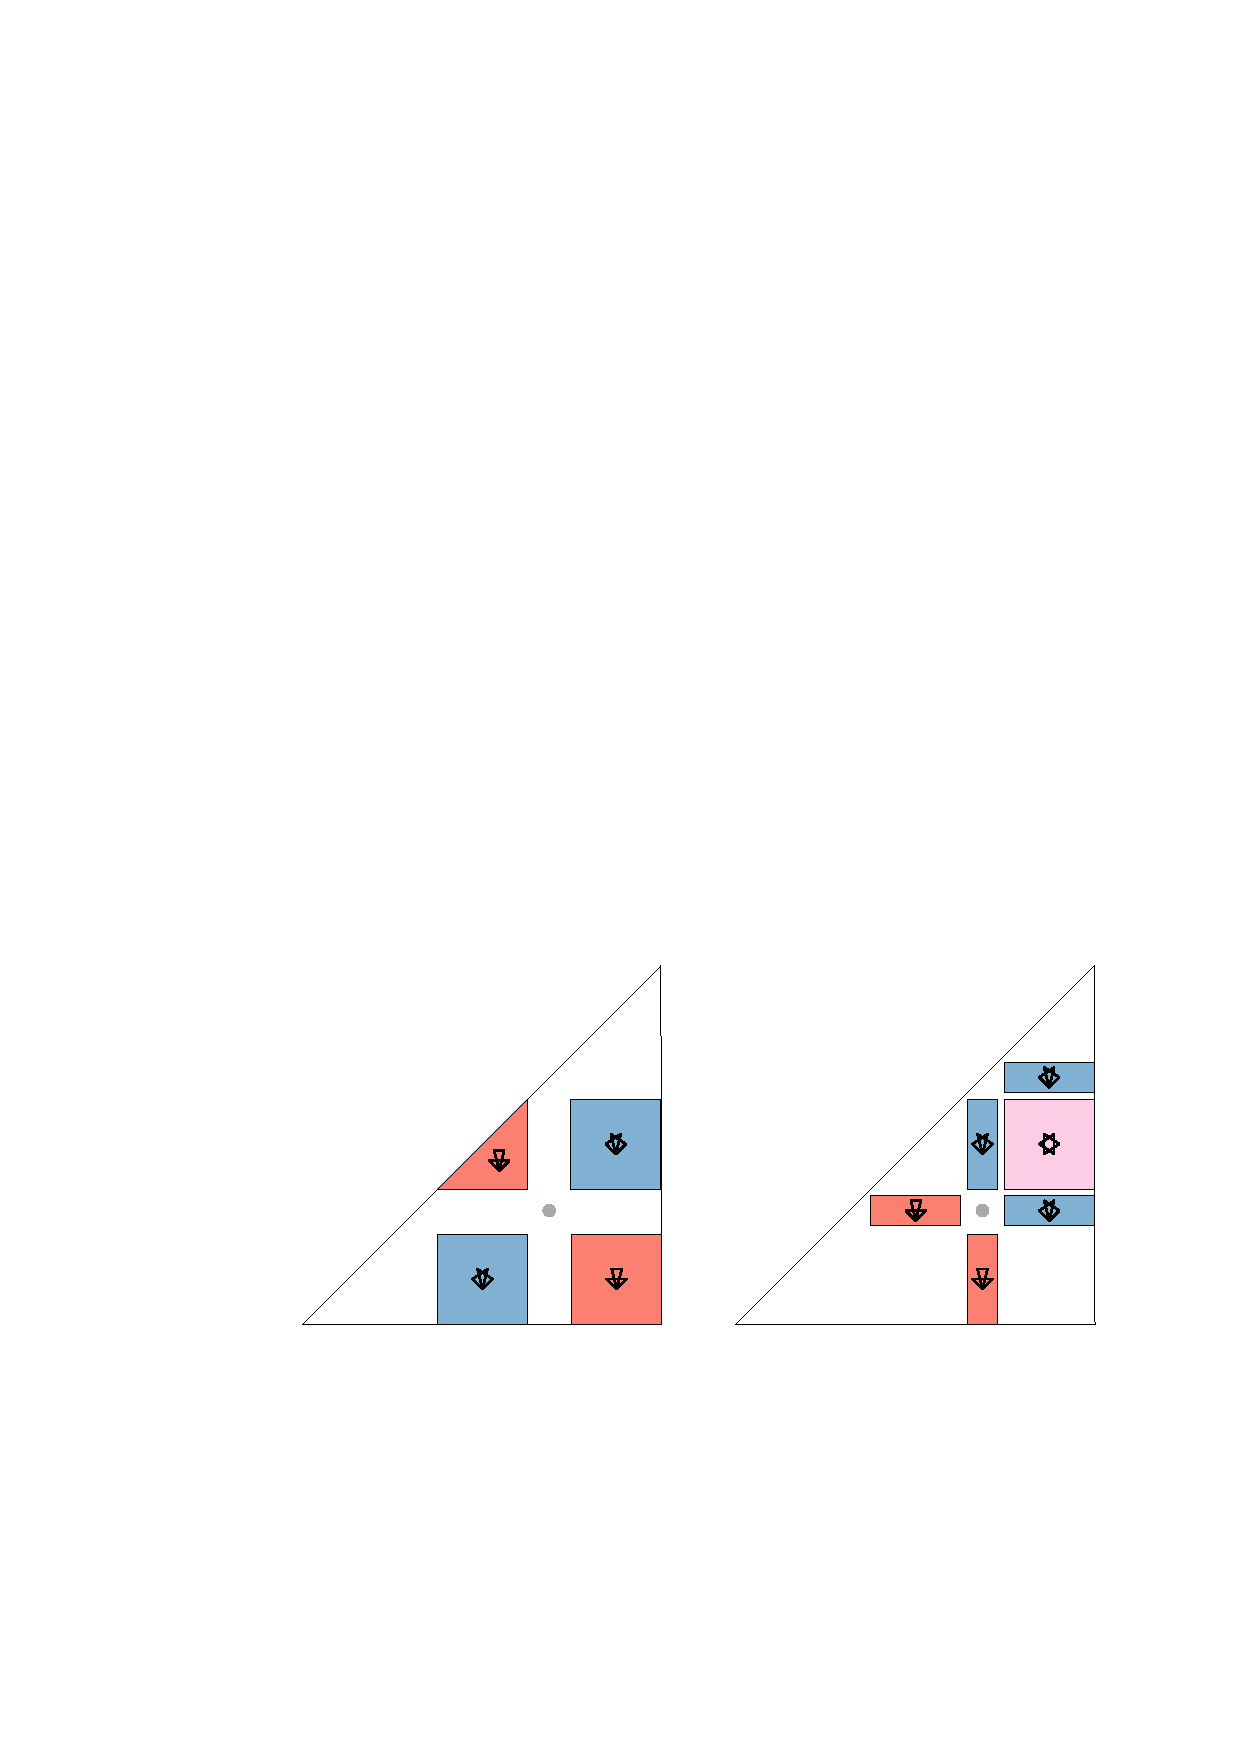
\includegraphics[height=3cm]{figs/helper-18}
\end{center}


\begin{proof}
   We repeatedly take points on the diagonal.
\end{proof}

\begin{thm}\thmlabel{bat-nested-ears}
  $\ex(n,\{\bat,\nested,\ears\}) \in \Theta(n^2)$.
\end{thm}
\begin{center}
   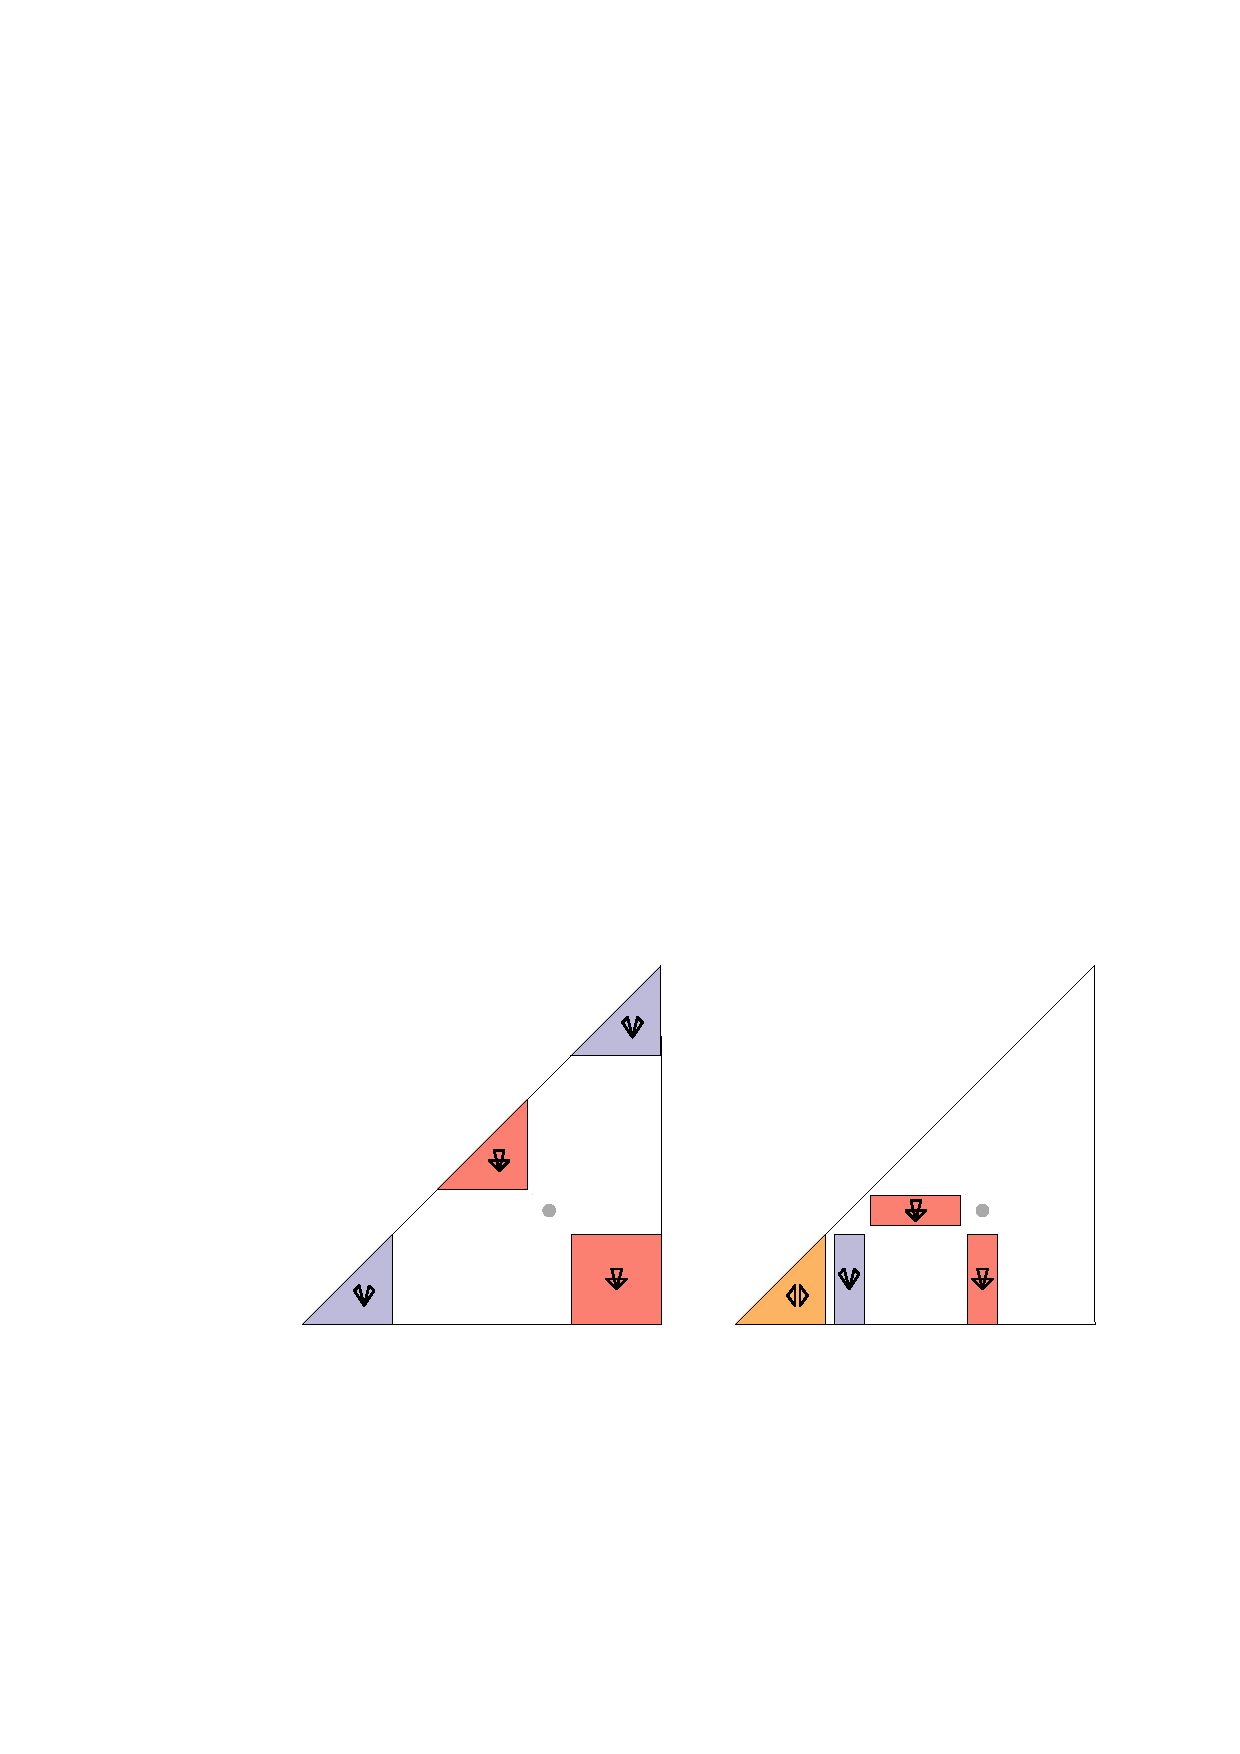
\includegraphics[height=3cm]{figs/helper-19}
\end{center}


\begin{proof}
   We repeatedly take points on the diagonal of the lower-right quadrant.
\end{proof}

\section*{Acknowledgement}

Some of this work was carried out at the Fourth Annual Workshop on
Geometry and Graphs, held at the Bellairs Research Institute in Barbados,
March 6--11, 2016. The authors are grateful to the organizers and to
the other participants of this workshop for providing a stimulating working
environment.


\bibliographystyle{plain}
\bibliography{turan}

\end{document}


